%%
%%  Department of Electrical, Electronic and Computer Engineering.
%%  EPR400/2 Final Report - Main File.
%%  Copyright (C) 2011-2021 University of Pretoria.
%%

\documentclass{epr400}

%% My packages, was not included in the template
\usepackage{algpseudocode}
\usepackage{subcaption}
\usepackage{siunitx} % For SI units
\usepackage{xfrac} % For slanted fractions \sfrac{}{}
\usepackage{fp} % For floating point calculations
\usepackage{pgfmath} % Include the pgfmath package
\usepackage{ulem}
\usepackage{tabularx}
\usepackage{enumitem}
\setlist[itemize]{topsep=3pt, partopsep=0pt, itemsep=0pt, parsep=0pt}
\usepackage{soul} % For highlighting text with \hl{}
\usepackage[hidelinks]{hyperref}
% Define autoref name for algorithms
\providecommand*{\algorithmautorefname}{Algorithm}

% This must be after hyperref.
\usepackage[acronym, nonumberlist, nopostdot]{glossaries} 
\loadglsentries{abbreviations}
\makeglossaries
% Define a custom glossary style
\newglossarystyle{epr_template_style}{
  \setglossarystyle{super} % base this style on the 'super' style
  % Spacing adjustments
  \renewenvironment{theglossary}
    {\begin{supertabular}{ @{} l p{\textwidth} }}
    {\end{supertabular}}
  \renewcommand{\acronymname}{\vspace{-1.2em}}
  \renewcommand{\glsgroupskip}{}
  \renewcommand*{\glossentry}[2]{
    \textbf{\glstarget{##1}{\glossentryname{##1}}} % Make abbreviation bold
    & \glossentrydesc{##1}\glspostdescription\space ##2\\
  }
}
\setglossarystyle{epr_template_style}


% Level 4 headings with \paragraph{
\setcounter{secnumdepth}{4}
\renewcommand\theparagraph{\alph{paragraph}}
\renewcommand\thesubparagraph{\arabic{subparagraph}}


%% EDIT: Replace the following with your information.
\eprtitle{Laser Pointer Turret Based Mosquito Air Defence System}
\eprcode{EPR402}
\eprcandidatename{A. Hartman}
\eprstudentnumber{20475323}
\eprdate{November 2023}
\eprsupervisor{Prof. P. de Villiers}
\eprcopynum{Electronic copy}

\begin{document}

%% Generate the required title page.
\maketitlepage

%% --- PART 1 ------------------------------------------------------------

\pagestyle{plain}
\pagenumbering{roman}

\eprsec{Part 1. Preamble}

\vspace*{0.5cm}

%% Import the required preamble pages.
%%
%%  Department of Electrical, Electronic and Computer Engineering.
%%  EPR400/2 Final Report - Preamble.
%%  Copyright (C) 2011-2021 University of Pretoria.
%%

This report describes work that I have completed in my final year project, developing a laser pointer turret based mosquito air defence system.
\\[2ex]
\textit{Project proposal and technical documentation} \newline
This main report contains an unaltered copy of the approved Project Proposal (as Part 2 of the report).

Technical documentation appears in Part 4 (Appendix).

All the code that I developed appears as a separate submission on the AMS.
\\[2ex]
\textit{Project history} \newline
This project does not extend on a previous project. The design and implementation is completely new.

I used library code for low level hardware interfacing with camera and motors. The implementation of the Hungarian algorithm was taken from an existing software module. The rest of the work reported on here, is entirely my own.
\\[2ex]
\textit{Language editing} \newline
This document has been language edited by a knowledgeable person. By submitting this document in its present form, I declare that this is the written material that I wish to be examined on.

My language editor was Ms. Michelle Hartman.

\vspace*{0.5cm}

\begin{tabular}{cp{4cm}ll}
  
\includegraphics[width=3.5cm]{figures/mich_handtekening.png} &  & \underline{\today} \\
  \textit{Language editor signature}                           &  & \textit{Date}
\end{tabular}

\vspace*{0.5cm}

\textit{Declaration}
\\[2ex]
I, \underline{\eprthecandidatename} understand what plagiarism is and have carefully studied the plagiarism policy of the University. I hereby declare that all the work described in this report is my own, except where explicitly indicated otherwise. Although I may have discussed the design and investigation with my study leader, fellow students or consulted various books, articles or the internet, the design/investigative work is my own. I have mastered the design and I have made all the required calculations in my lab book (and/or they are reflected in this report) to authenticate this. I am not presenting a complete solution of someone else.

Wherever I have used information from other sources, I have given credit by proper and complete referencing of the source material so that it can be clearly discerned what is my own work and what was quoted from other sources. I acknowledge that failure to comply with the instructions regarding referencing will be regarded as plagiarism.  If there is any doubt about the authenticity of my work, I am willing to attend an oral ancillary examination/evaluation about the work.

I certify that the Project Proposal appearing as the Introduction section of the report is a verbatim copy of the approved Project Proposal.

\begin{tabular}{cp{5cm}ll}
  
\includegraphics[width=3.5cm]{figures/anton_handtekening.png} &  & \underline{\today} \\
  \eprthecandidatename                                          &  & Date
\end{tabular}

%% End of File.


\newpage

%% Add the Table of Contents.
\makeatletter
\renewcommand\@dotsep{200}
\makeatother
\tableofcontents
\thispagestyle{empty}
\newpage

%% Print the list of abbrieviations.
\printglossary[type=\acronymtype, title={LIST OF ABBREVIATIONS}]
\newpage

%% --- PART 2 ------------------------------------------------------------

\eprsec{Part 2. Project definition: approved Project Proposal}

This section contains the problem identification in the form of the complete approved Project Proposal, unaltered from the final approved version that appears on the AMS.

\newpage

%% Import the approved project proposal
% 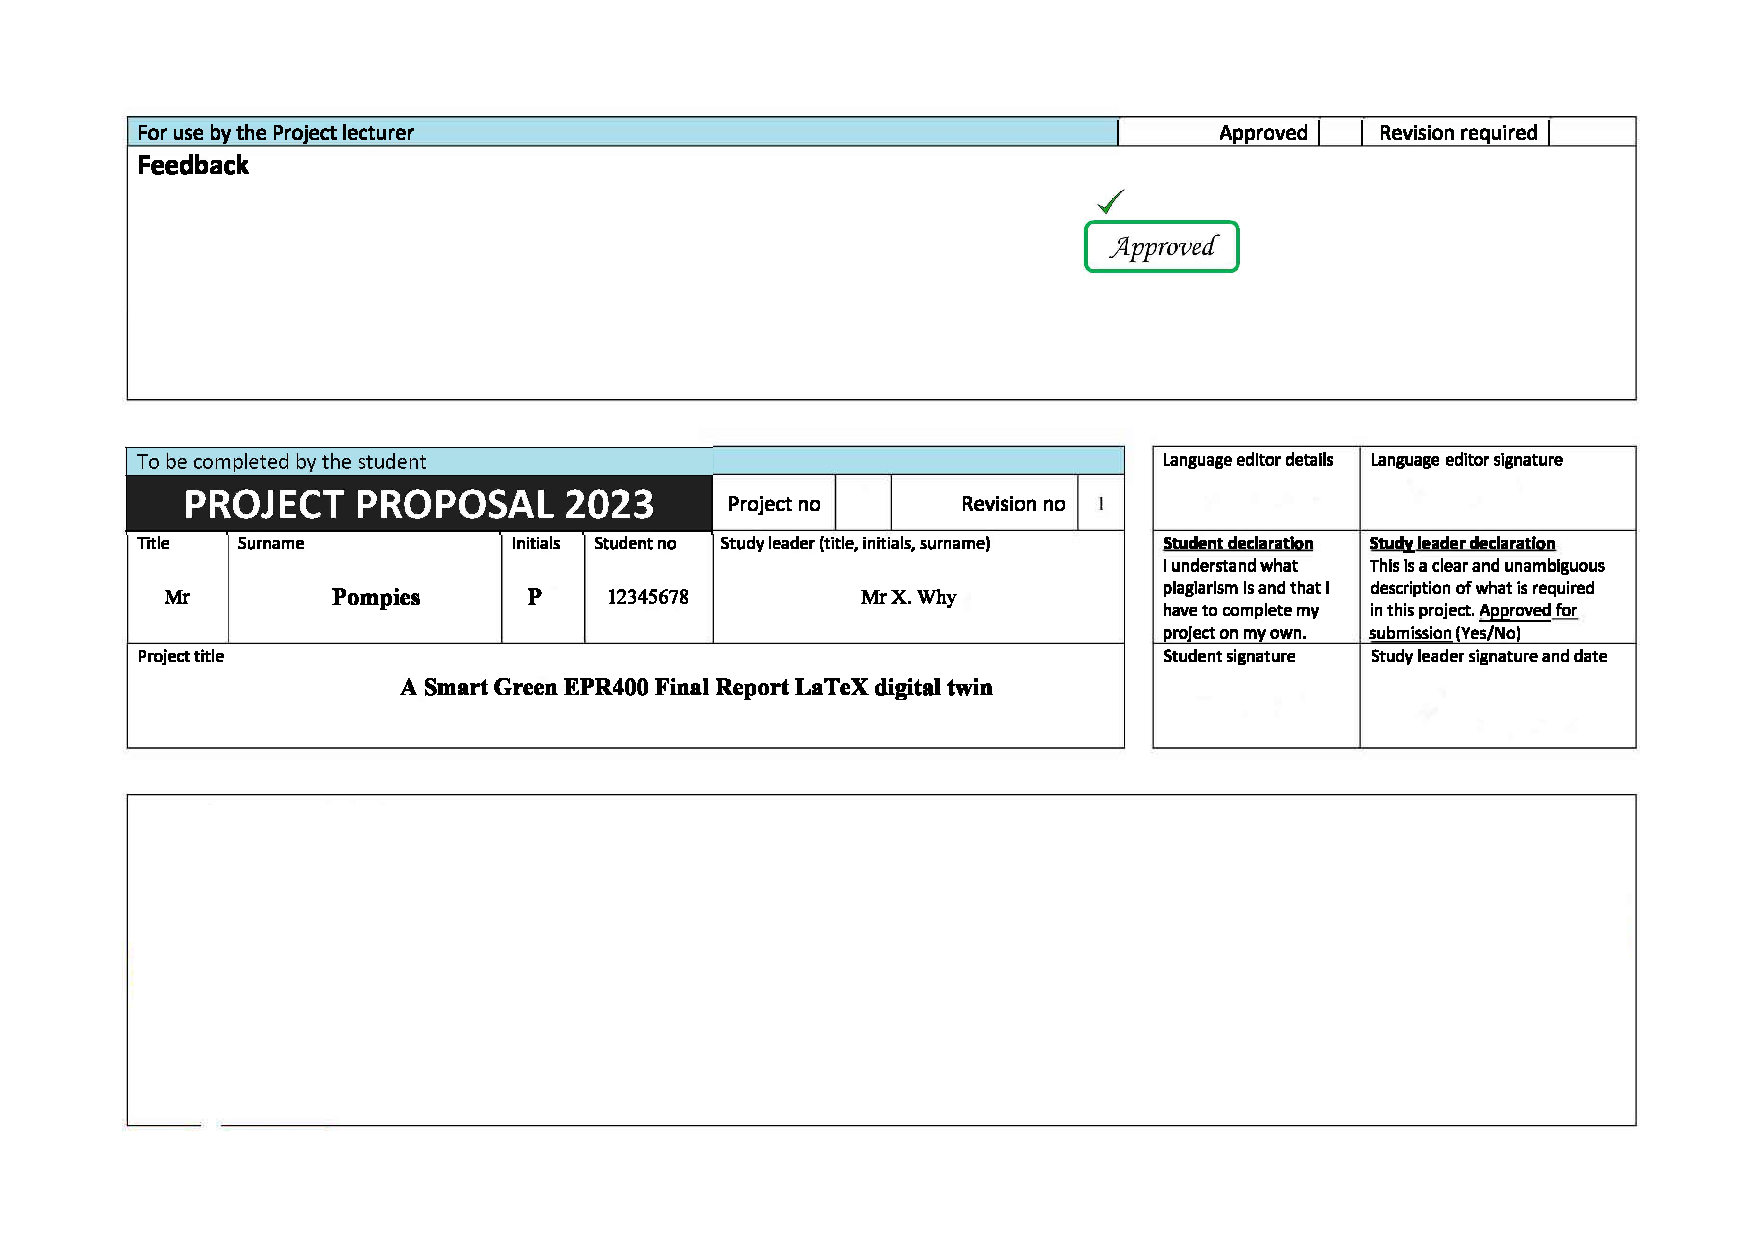
\includepdf[pages=-, angle=90]{ApprovedProposal.pdf}
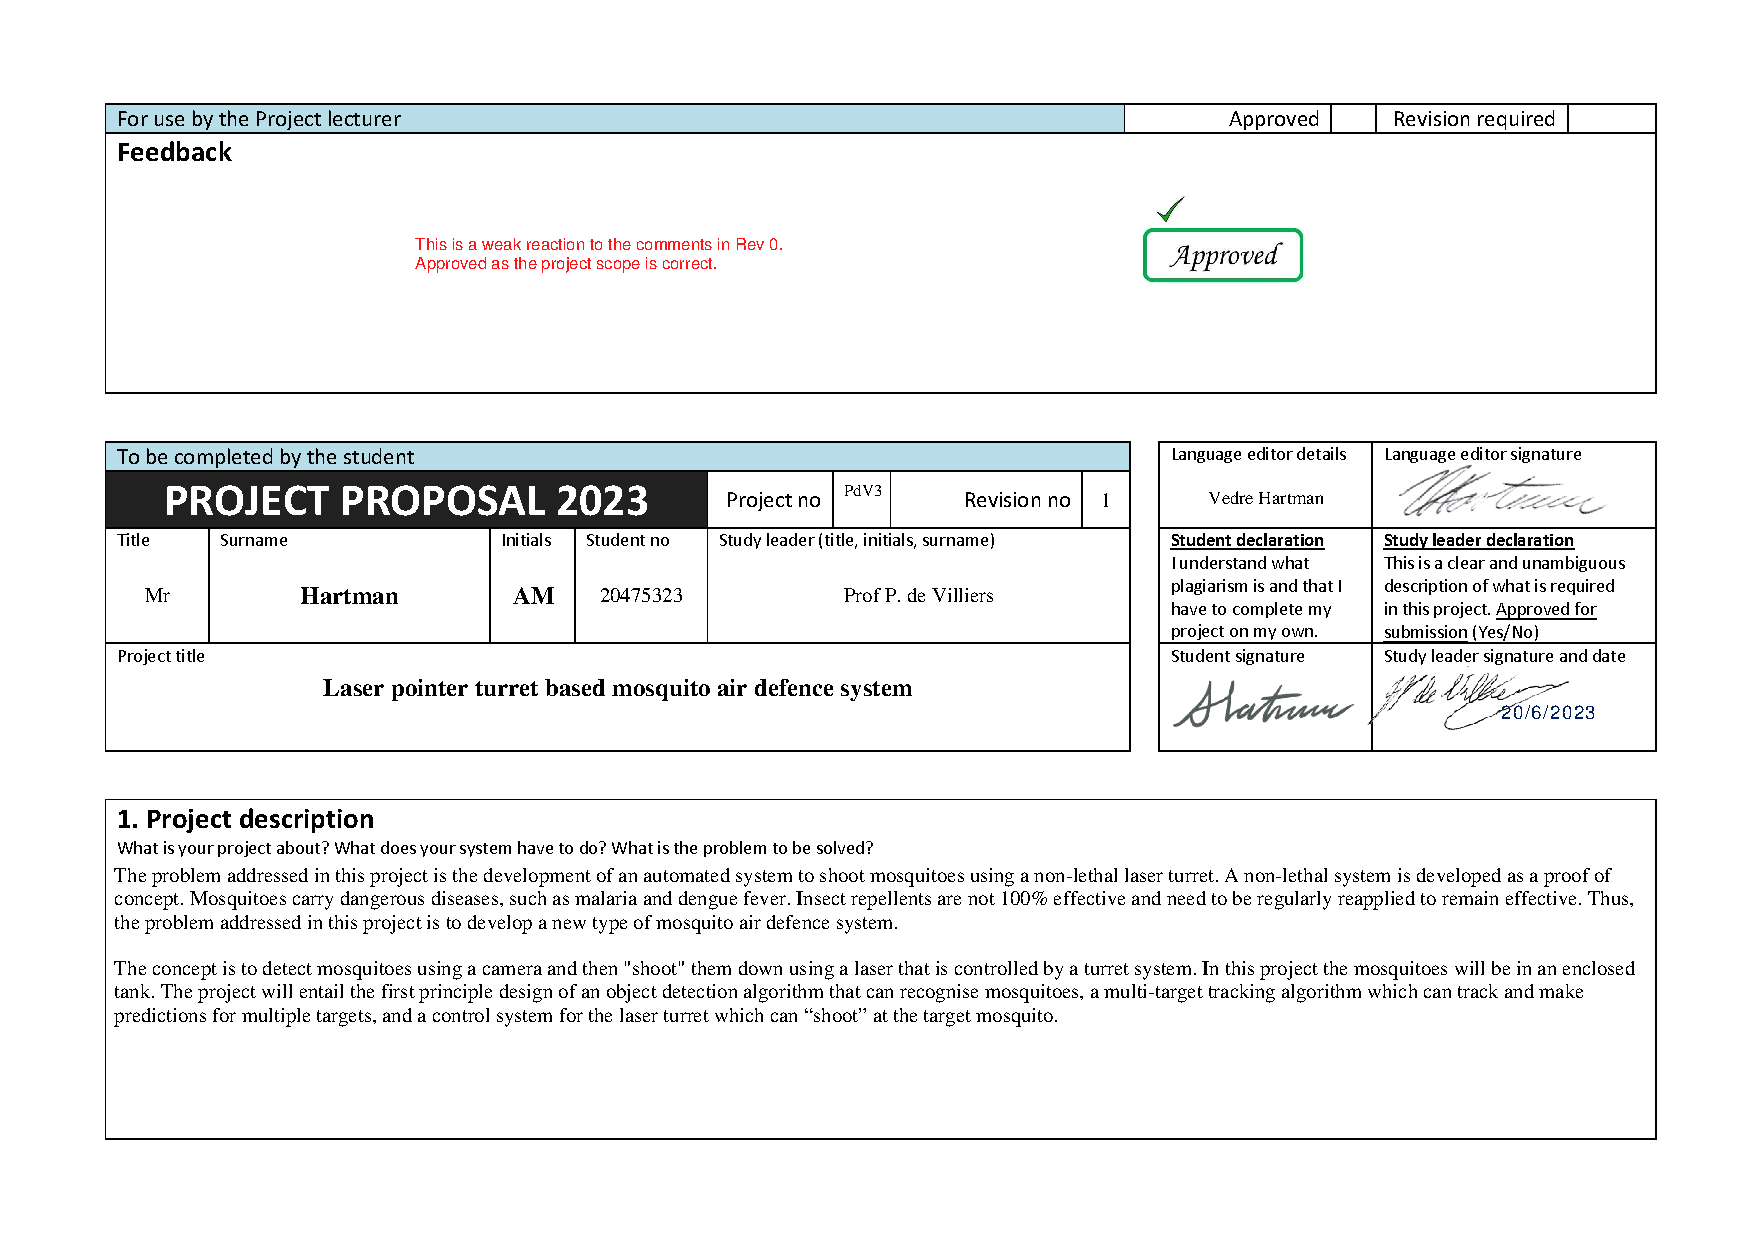
\includepdf[pages=-, angle=90]{HartmanAM_20475323_R1_FEEDBACK_Comments_Romoved.pdf}

\addtocontents{toc}{\protect\contentsline{subsection}{1. Project description}{}\%}
\addtocontents{toc}{\protect\contentsline{subsection}{2. Technical challenges in this project}{}\%}
\addtocontents{toc}{\protect\contentsline{subsection}{3. Functional analysis}{}\%}
\addtocontents{toc}{\protect\contentsline{subsection}{4. System requirements and specifications}{}\%}
\addtocontents{toc}{\protect\contentsline{subsection}{5. Field conditions}{}\%}
\addtocontents{toc}{\protect\contentsline{subsection}{6. Student tasks}{}\%}

%% --- PART 3 ------------------------------------------------------------

\eprsec{Part 3. Main Report}
\newpage

%% Reset the page number style and count.
\pagenumbering{arabic}
\setcounter{page}{1}

%% Import the main report content
%%
%%  Department of Electrical, Electronic and Computer Engineering.
%%  EPR400/2 Final Report - Section 1.
%%  Copyright (C) 2011-2021 University of Pretoria.
%%

\section{Literature study}

Shannon {\it et al.}\cite{Shannon:A_Mathematical_Theory_of_Communications}


\newpage

%% End of File.



%%
%%  Department of Electrical, Electronic and Computer Engineering.
%%  EPR400/2 Final Report - Section 2.
%%  Copyright (C) 2011-2021 University of Pretoria.
%%

\section{Approach}
The aim of this project was to develop a system that would track and  illuminate mosquitoes with a laser. The system will detect mosquitoes using a camera and the laser will be controlled by a turret system. The system is implicitly required to operate in real-time in order to track and illuminate mosquitoes with a laser. This was taken into consideration in all the design aspects of the system. The project entails the first principles design of the following:
\begin{itemize}
  \item A laser turret that can change the position of a laser beam.
  \item A control system that can control the laser turret.
  \item An object detection algorithm that can detect mosquitoes.
  \item An object detection algorithm that can detect the reflections of the laser beam.
  \item A multi-target tracking algorithm that can track multiple mosquitoes and predict their future locations.
\end{itemize}

The laser turret was inspired by two-axis laser scanners that use two mirrors to direct a laser beam in two dimensions as illustrated in \autoref{fig:two-axis-scanner-schematic}. The advantages of this approach compared to moving that laser diode itself is that the mirrors are rotated about their centre of mass which reduces the torque required to rotate the mirrors. This enables the laser turret to rapidly change the position of the mirrors and in tern the position of the laser beam. The drawback of this approach is that there will be additional scattering of the laser beam due to imperfections in the mirrors. This will not have significant impact on the system, therefore, this approach was chosen for the laser turret. A closed-loop \gls{pid} control system will be used to control the laser turret. The laser position feedback for the control system will be provided by the laser detection system.

The object detection algorithm to detect mosquitoes can be implemented using a deep learning approach that will enable the identification and appearance matching of mosquitoes. This approach is computationally expensive and will require quality high-resolution images of mosquitoes. A less computational expensive approach is to use image segmentation techniques to separate the mosquitoes from the background of the image. An image segmentation approach greatly reduces the computational complexity at the expense of flexibility and robustness. Another trade-off to consider is that this approach will not be able to distinguish between mosquitoes and other objects similar in appearance. Image segmentation does not require the same quality and resolution images as a deep learning approach since it will not distinguish between objects of similar appearance. The benefits of an image segmentation approach outweigh the trade-offs compared to a deep learning approach for this project. Therefore, the image segmentation approach was chosen for this project.

The same considerations were made for the object detection algorithm to detect the reflections of the laser beam. An image segmentation approach was chosen for the same reasons as discussed above.

The multi-target tracking algorithm is required to track and predict the locations of mosquitoes. This can be efficiently achieved using a Kalman filter for one object. The Kalman filter is a recursive algorithm that can be used to estimate the state of a system that is subject to random noise. The Kalman filter is able to recursively predict the future state of a system, which is required to predict the future locations of a mosquito. This can be extended to track multiple objects using the \gls{sort} algorithm that combines the Kalman filter and the Hungarian algorithm. The Hungarian algorithm is an optimal assignment algorithm that can be used to assign detections to tracks. The \gls{sort} algorithm is less computationally complex than other multi-target tracking algorithms while maintaining a comparable or higher accuracy \cite{SORT-Bewley2017}.

A high-level overview of the system can be seen in \autoref{fig:system_overview}. The system was designed to operate in a controlled environment.
\begin{figure}[h]
  \centering
  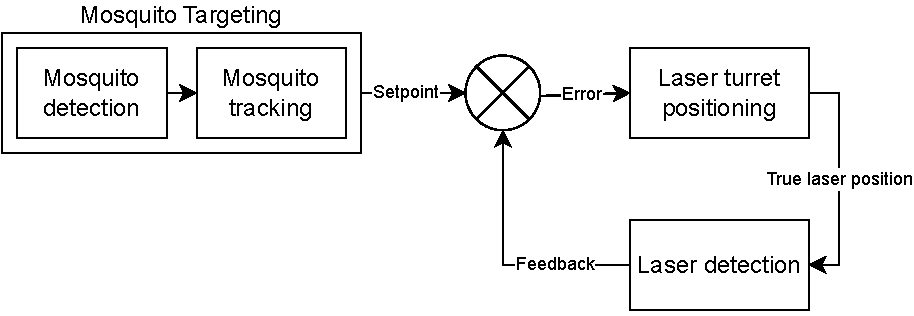
\includegraphics[width=1\textwidth]{figures/system_overview.pdf}
  \caption{Overview of the system.}
  \label{fig:system_overview}
\end{figure}

\newpage

%% End of File.


%%
%%  Department of Electrical, Electronic and Computer Engineering.
%%  EPR400/2 Final Report - Section 3.
%%  Copyright (C) 2011-2021 University of Pretoria.
%%

\section{Design and implementation}
\subsection{Design summary}
This section summarises the project design tasks and how they were
implemented (see \autoref{tab:design_summary}).
\begin{table}[!htb]
  \centering
  \begin{tabularx}{\textwidth}{|X|X|X|}
    \hline
    \textbf{Deliverable or task}                                                                                          & \textbf{Implementation}                                                                               &
    \textbf{Completion of deliverable or task, and section in the report}
    \\
    \hline
    The laser turret and laser turret control system had to be designed and implemented by the student.                   & The laser turret and laser turret control system were designed and implemented from first principles. & Completed. \newline \Cref{subsec:hardware_design,subsec:hardware_implementation,subsec:software_design,subsec:software_implementation}
    \\
    \hline
    The mosquito and laser detection algorithm had to be designed and implemented on an embedded platform by the student. & The mosquito and laser detection algorithm was designed and implemented from first principles.        & Completed. \newline \Cref{subsec:software_design,subsec:software_implementation}
    \\
    \hline
    The mosquito tracking and prediction algorithm had to be developed and implemented by the student.                    & The mosquito tracking algorithm and prediction was developed and implemented from first principles.   & Completed. \newline \Cref{subsec:software_design,subsec:software_implementation}
    \\
    \hline
    An appropriate camera had to be selected by the student.                                                              & An appropriate camera was selected by the student.                                                    & Completed. \newline \Cref{subsubsec:camera_selection}
    \\
    \hline
  \end{tabularx}
  \caption{Design summary.}
  \label{tab:design_summary}
\end{table}


\subsection{Theoretical analysis and modelling}

\subsubsection{Mapping pixel co-ordinates to metric co-ordinates}
To control the laser, its position must be known in the world co-ordinate frame. The laser position was measured using a camera, thus the camera's pixel co-ordinate frame must be mapped to the world co-ordinate frame. To perform this mapping a camera model is required. The forward imaging model of a camera is shown in \autoref{fig:camera_forward_imaging_model}.
\begin{figure}[!htb]
  \centering
  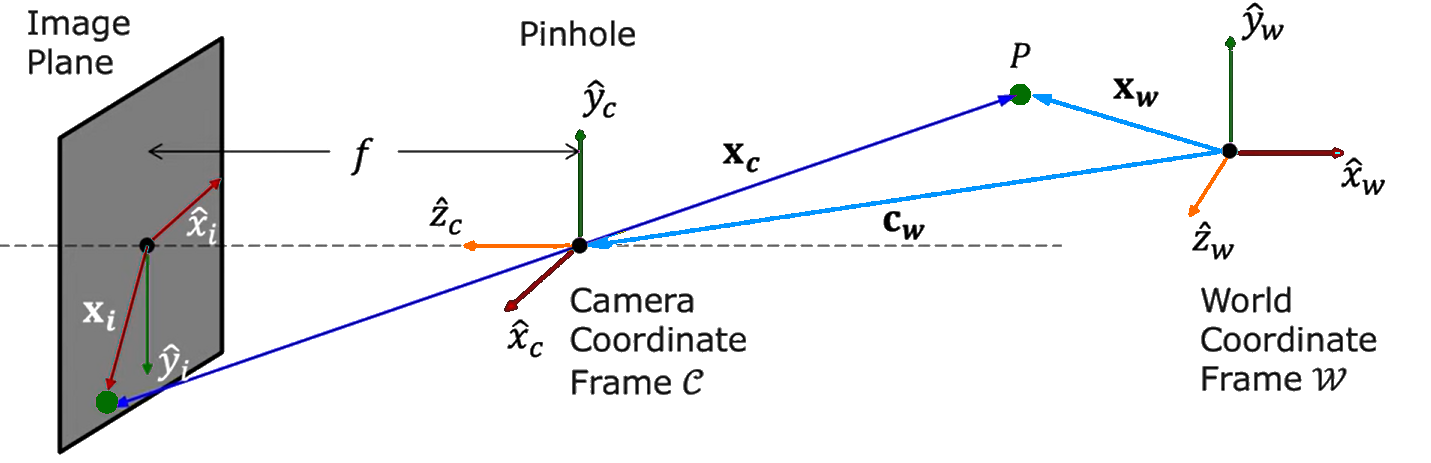
\includegraphics[width=0.95\textwidth]{figures/camera/wit_forward_imaging_model.png}
  \caption{Forward imaging model of a camera. This figure was modified from \cite{Nayar}.}
  \label{fig:camera_forward_imaging_model}
\end{figure}

Using the forward imaging model the pixel distance was mapped to the metric distance for the $x$-axis with
\begin{equation}
  X = Z \times \left( \frac{x - x_{ref}}{f_x} \right)\,,
  \label{eq:pixel_to_metric}
\end{equation}
where $Z$ is the depth camera with respect to the world co-ordinate frame, $x$ is the pixel of interest, $x_{ref}$ is the reference pixel, and $f_x$ is the effective focal length of the camera. Similarly, the pixel distance was mapped to the metric distance for the y-axis. The effective focal length of the camera $f_x$ was determined through camera calibration. The mapping is performed for the $y$-axis.


\subsubsection{Morphological operations}
\label{subsubsec:morphological_operations}
Erosion is a fundamental morphological operation used to remove small structures or details from a binary image. It is defined as the basic set operation of moving a structuring element (usually a smaller binary matrix) over the input binary image and finding the intersection of the structuring element with the image. This operation can be mathematically expressed as
\begin{equation}
  (A \ominus B)(x, y) = \bigcap \{A(x + i, y + j) | (i, j) \in B\}\,,
  \label{eq:erosion}
\end{equation}
where
\begin{itemize}
  \item $A$ is the input binary image.
  \item $B$ is the structuring element.
  \item $\ominus$ represents the erosion operation.
  \item $(x, y)$ are the pixel co-ordinates in the resulting image.
\end{itemize}

Dilation is another fundamental morphological operation, but it is used to enhance or grow the features in a binary image. Dilation can be defined as the set operation that moves the structuring element over the input image and computes the union of the element with the parts of the image where the structuring element "hits". The mathematical expression for dilation is as follows:
\begin{equation}
  (A \oplus B)(x, y) = \bigcup \{A(x + i, y + j) | (i, j) \in B\}
  \label{eq:dilation}
\end{equation}
where
\begin{itemize}
  \item $A$ is the input binary image.
  \item $B$ is the structuring element.
  \item $\oplus$ represents the dilation operation.
  \item $(x, y)$ are the pixel co-ordinates in the resulting image.
\end{itemize}

The erosion and dilation operations are illustrated in \autoref{fig:erosion_and_dilation}.
\begin{figure}[!htb]
  \centering
  \begin{subfigure}[t]{0.45\textwidth}
    \centering
    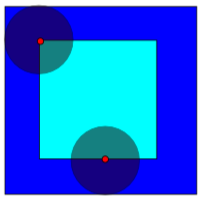
\includegraphics[width=0.5\linewidth]{figures/detection/erosion.png}
    \caption{The erosion of the dark-blue square by a disk, resulting in the light-blue square.}
    \label{fig:erosion}
  \end{subfigure}
  \quad
  \begin{subfigure}[t]{0.45\textwidth}
    \centering
    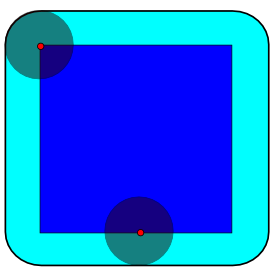
\includegraphics[width=0.5\linewidth]{figures/detection/dilation.png}
    \caption{The dilation of a dark-blue square by a disk, resulting in the light-blue square with rounded corners.}
    \label{fig:dilation}
  \end{subfigure}
  \caption{The figure shows an example of erosion and dilation. This figure was modified from \cite{Renatokeshet_2023}.}
  \label{fig:erosion_and_dilation}
\end{figure}

Opening is a compound morphological operation that consists of an erosion followed by a dilation using the same structuring element. It is primarily used to remove noise and small objects from a binary image. The opening of an image $A$ by a structuring element $B$ is defined as
\begin{equation}
  A \circ B = (A \ominus B) \oplus B\,,
  \label{eq:opening}
\end{equation}
where
\begin{itemize}
  \item $A$ is the input binary image.
  \item $B$ is the structuring element.
  \item $\circ$ represents the opening operation.
\end{itemize}

Closing is another compound morphological operation that consists of dilation followed by an erosion using the same structuring element. It is used to close small holes and gaps in objects and to connect nearby objects. The closing of an image $A$ by a structuring element $B$ is defined as
\begin{equation}
  A \bullet B = (A \oplus B) \ominus B\,,
  \label{eq:closing}
\end{equation}
where
\begin{itemize}
  \item $A$ is the input binary image.
  \item $B$ is the structuring element.
  \item $\bullet$ represents the closing operation.
\end{itemize}

Opening and closing are both idempotent operations, meaning that repeated openings or closing have no effect on the image. Opening and closing is illustrated in \autoref{fig:opening_and_closing}.
\begin{figure}[!htb]
  \centering
  \begin{subfigure}[t]{0.45\textwidth}
    \centering
    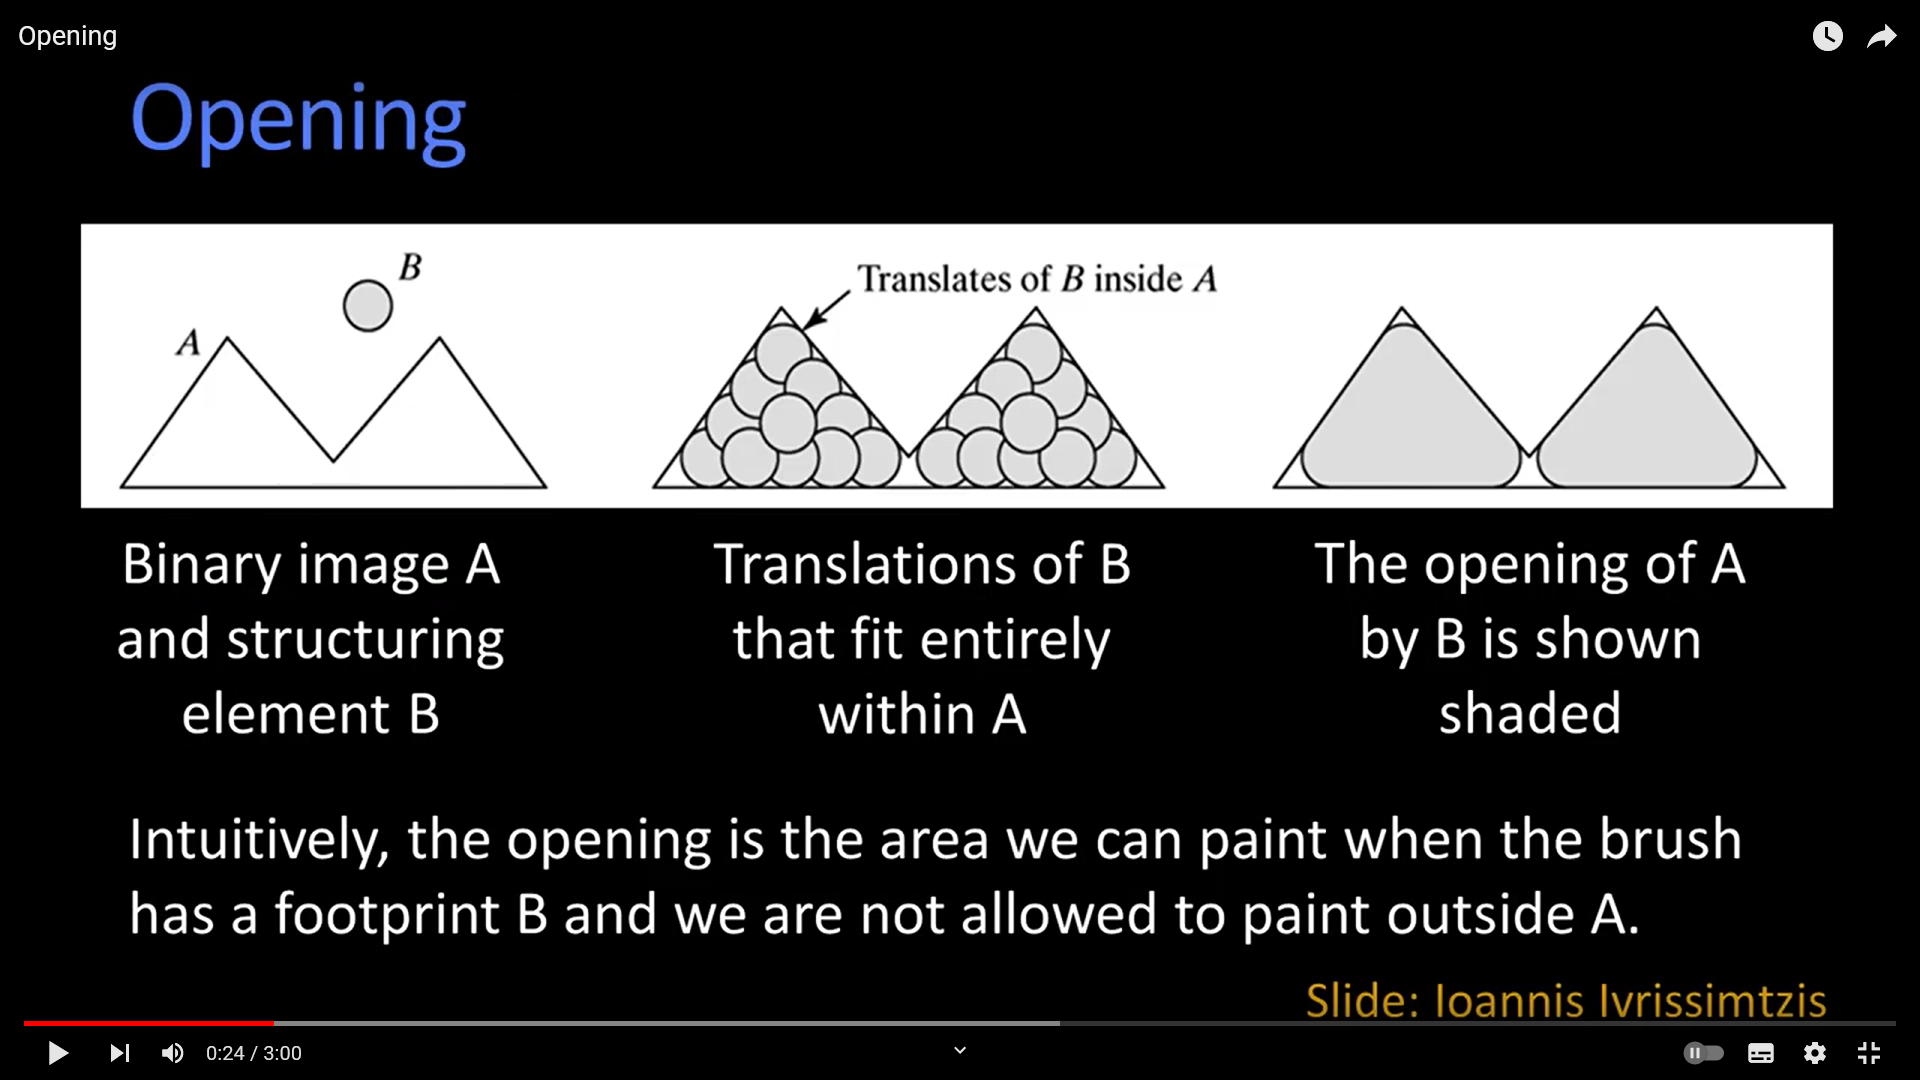
\includegraphics[width=0.5\linewidth]{figures/detection/opening.png}
    \caption{The opening of the dark-blue square by a disk, resulting in the light-blue square with round corners.}
    \label{fig:opening}
  \end{subfigure}
  \quad
  \begin{subfigure}[t]{0.45\textwidth}
    \centering
    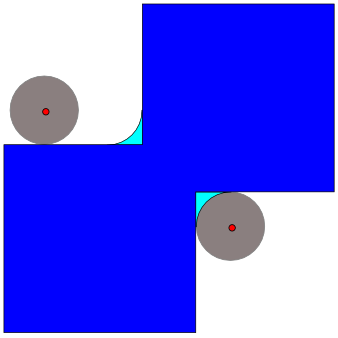
\includegraphics[width=0.5\linewidth]{figures/detection/closing.png}
    \caption{The closing of the dark-blue shape (union of two squares) by a disk, resulting in the union of the dark-blue shape and the light-blue areas.}
    \label{fig:closing}
  \end{subfigure}
  \caption{The figure shows and example of opening and closing. This figure was modified from \cite{Renatokeshet_2023}.}
  \label{fig:opening_and_closing}
\end{figure}

\subsubsection{Kalman filter} \label{subsubsec:kalman_filter}
The Kalman filter is a recursive algorithm that estimates the state of a system from a series of noisy measurements. The Kalman filter is based on a linear dynamical system model, which is defined by the following equations:
\begin{equation}
  \begin{aligned}
    \mathbf{x}_k & = \mathbf{Ax}_{k - 1} + \mathbf{Bu}_{k - 1} + \mathbf{w}_{k - 1}\,, \\
    \mathbf{z}_k & = \mathbf{Hx}_k + \mathbf{v}_k\,,
  \end{aligned}
  \label{eq:kalman_filter}
\end{equation}
where
\begin{itemize}
  \item $\mathbf{x}_k$ is the state vector at time $k$.
  \item $\mathbf{z}_k$ is the measurement vector at time $k$.
  \item $\mathbf{A}$ is the state transition matrix.
  \item $\mathbf{B}$ is the control matrix.
  \item $\mathbf{u}_k$ is the control vector at time $k$.
  \item $\mathbf{w}_k$ is the process noise vector at time $k$.
  \item $\mathbf{H}$ is the observation matrix.
  \item $\mathbf{v}_k$ is the measurement noise vector at time $k$.
\end{itemize}

The Kalman filter algorithm can be divided into two phases: the prediction phase and the update phase. The equations for the prediction phase is
\begin{equation}
  \begin{aligned}
    \hat{\mathbf{x}}_k^- & = \mathbf{A}\hat{\mathbf{x}}_{k - 1} + \mathbf{B}\mathbf{u}_{k - 1}\,, \\
    \mathbf{P}_k^-       & = \mathbf{AP}_{k - 1}\mathbf{A}^T + \mathbf{Q}\,,
  \end{aligned}
  \label{eq:kalman_filter_prediction}
\end{equation}
where
\begin{itemize}
  \item $\hat{\mathbf{x}}_k^-$ is the a priori state estimate at time $k$.
  \item $\mathbf{P}_k^-$ is the a priori error covariance matrix at time $k$.
  \item $\mathbf{Q}$ is the process noise covariance matrix.
\end{itemize}

The equations for the update phase is
\begin{equation}
  \begin{aligned}
    \mathbf{K}_k       & = \mathbf{P}_k^-\mathbf{H}^T(\mathbf{HP}_k^-\mathbf{H}^T + \mathbf{R})^{-1}\,,          \\
    \hat{\mathbf{x}}_k & = \hat{\mathbf{x}}_k^- + \mathbf{K}_k(\mathbf{z}_k - \mathbf{H}\hat{\mathbf{x}}_k^-)\,, \\
    \mathbf{P}_k       & = (\mathbf{I} - \mathbf{K}_k\mathbf{H})\mathbf{P}_k^-\,,
  \end{aligned}
  \label{eq:kalman_filter_update}
\end{equation}
where
\begin{itemize}
  \item $\mathbf{K}_k$ is the Kalman gain at time $k$.
  \item $\hat{\mathbf{x}}_k$ is the a posteriori state estimate at time $k$.
  \item $\mathbf{P}_k$ is the a posteriori error covariance matrix at time $k$.
  \item $\mathbf{R}$ is the measurement noise covariance matrix.
\end{itemize}

The Kalman filter, initialised with an initial state estimate $\hat{\mathbf{x}}_0$ and error covariance $\mathbf{P}_0$, is a recursive, adaptive, and linear estimator that optimally minimises the mean square error for real-time state estimation of linear systems with computational efficiency.

\FloatBarrier
\subsection{Hardware design}\label{subsec:hardware_design}
The hardware block diagram is presented in \autoref{fig:hardware_block}. The hardware consists primarily of a laser turret, a camera, a mosquito enclosure, and an embedded processing platform. The laser turret is used to move the laser beam across the mosquito enclosure. The camera is used to detect the laser beam and the mosquitoes. A bracket is used to position the laser turret and the camera relative to the mosquito enclosure. The embedded processing platform is used to control the laser turret and perform the image processing required for the laser detection and mosquito detection.
\begin{figure}[!htb]
  \centering
  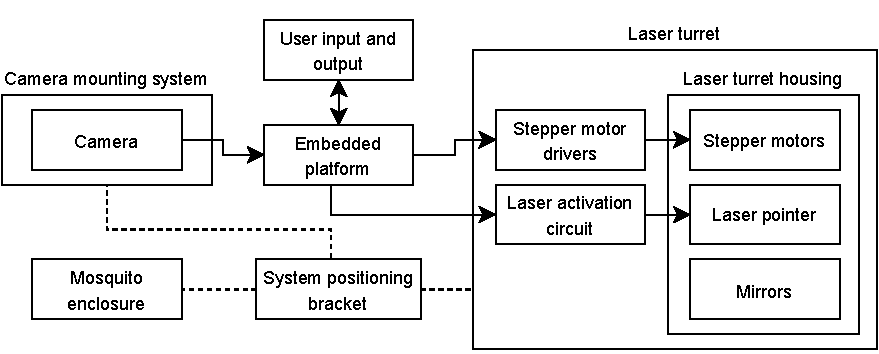
\includegraphics[width=\textwidth]{figures/hardware_block_diagram.pdf}
  \caption{Hardware block diagram.}
  \label{fig:hardware_block}
\end{figure}



\subsubsection{Embedded platform selection}
To select an embedded platform for the project the following requirements were considered:
\begin{description}[style=nextline]
  \item[Processing power] The embedded platform must be able to perform the image processing required for the laser detection and mosquito detection in real-time. Image processing is computationally intensive, but can largely benefit from parallelisation. Therefore, an embedded platform with a \gls{gpu} will be preferred.
  \item[Memory] The embedded platform must have sufficient memory to store the multiple images along with the required algorithms. A 1080p image with three 8-bit colour channels requires 6 MB of memory.
  \item[Hardware interfaces] The embedded platform must be compatible with camera interfaces. It must also have sufficient \gls{gpio} pins to interface with the stepper motor drivers. The embedded platform must also have support for a display output and a keyboard and mouse input to provide a user interface to control the system.
  \item[Availability and support] It is import to select an embedded platform that is readily available. It is important to select an embedded platform with large body of knowledge available and sufficient scientific support community since this is an individual project without access to people with expertise with the embedded platform.
\end{description}

The Nvidia Jetson Nano was chosen as the embedded platform for the project. The Nvidia Jetson Nano is a single-board computer with a \gls{gpu} and a quad-core \gls{cpu}. The Nvidia Jetson Nano has a \gls{mipi} \gls{csi}-2 camera interface and has 40 \gls{gpio} pins. The Jetson Nano has a quad-core ARM Cortex-A57 MPCore processor, an Nvidia Maxwell \gls{gpu} with 128 \gls{cuda} cores, and 4 GB of LPDDR4 memory. It also features an HDMI display output and a USB 3.0 port. The Nvidia Jetson Nano is readily available and has a large body of knowledge available and sufficient scientific support community.



\subsubsection{Camera selection}\label{subsubsec:camera_selection}
To minimise the computational complexity of the image processing required for the laser detection and mosquito detection a low video resolution will be used. The video resolution will not need to exceed 1080p. The camera must be able to capture images at a frame rate of at least 30 frames per second. The camera must also be compatible with the \gls{mipi} \gls{csi}-2 interface on the Nvidia Jetson Nano.

The Raspberry Pi Camera Module V2 was chosen as the camera for the project. The Raspberry Pi Camera Module V2 is an 8 MP camera that can capture images at a frame rate of 30 frames per second at 1080p. The Raspberry Pi Camera Module V2 is compatible with the \gls{mipi} \gls{csi} on the Nvidia Jetson Nano. The Raspberry Pi Camera Module V2 is readily available and has a large body of knowledge available and sufficient scientific support community.



\subsubsection{Mosquito enclosure}
The mosquito enclosure will be a rectangular prism as shown in \autoref{fig:mosquito_enclosure_dimensions}. The front facing surface will be transparent and the rest of the surfaces will be white. The enclosure will be fitted with internal lighting to ensure contrast between the background and the mosquitoes and to minimise the camera noise.
\begin{figure}[!htb]
  \centering
  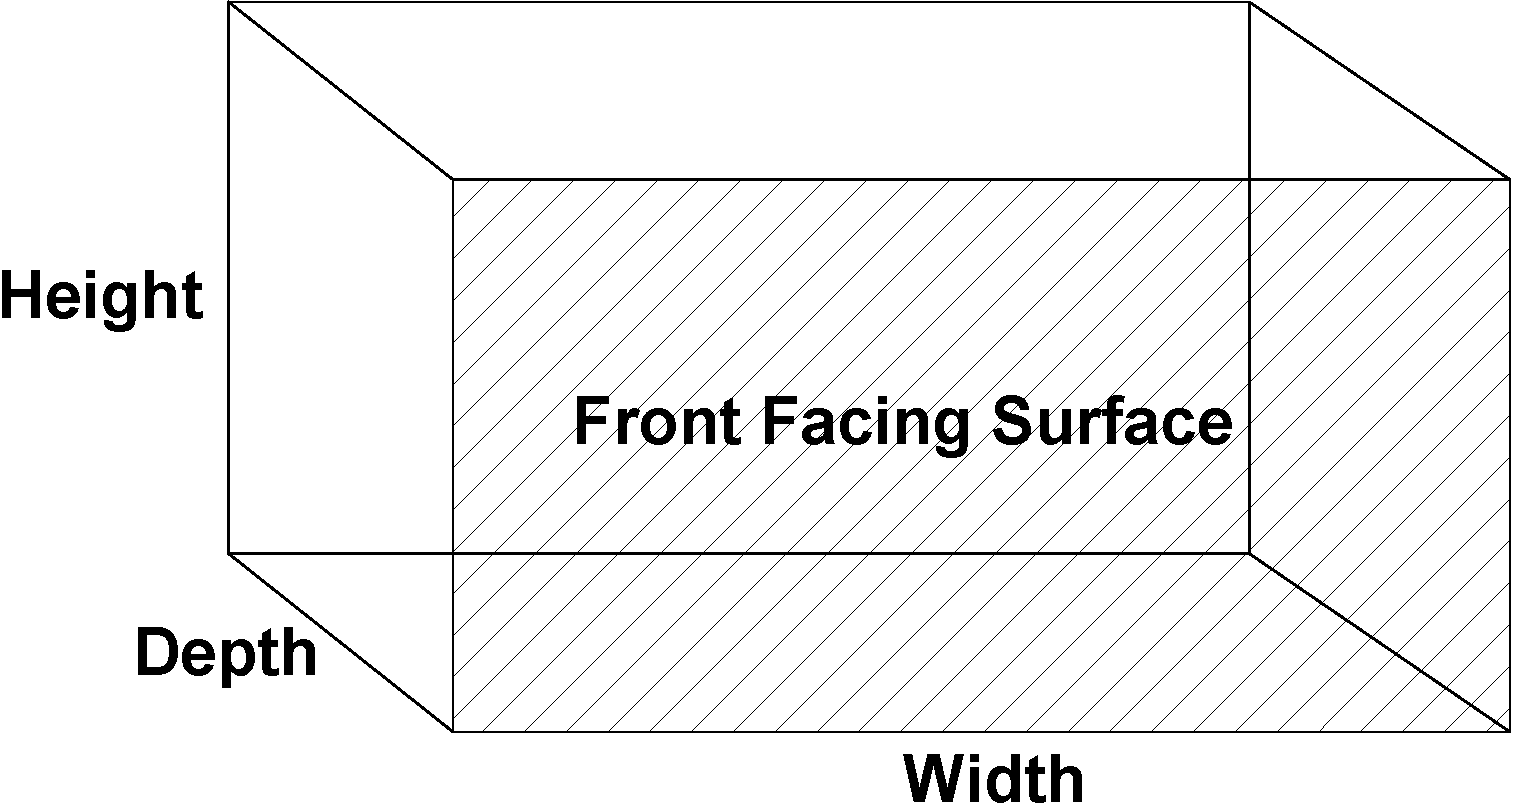
\includegraphics[width=0.6\textwidth]{figures/hardware_design/mos_enclosure.pdf}
  \caption{Mosquito enclosure.}
  \label{fig:mosquito_enclosure_dimensions}
\end{figure}



\subsubsection{Laser turret}\label{subsubsec:laser_turret_implementation}
The laser turret design was inspired by commercial two-axis laser scanners. The position of the laser beam is controlled by adjusting the angles of two mirrors. This is illustrated in \autoref{fig:two-axis-scanner-schematic}. The mirrors are connected directly to the output shaft of the motors. The laser turret will be positioned orthogonally to the $xy$-plane of the mosquito enclosure. The point where the laser beam shines orthogonal to the $xy$-plane of the mosquito enclosure is considered the origin of the laser. This will occur when the two mirrors are at 45$\degree$ relative to the laser beam.
\begin{figure}[!htb]
  \centering
  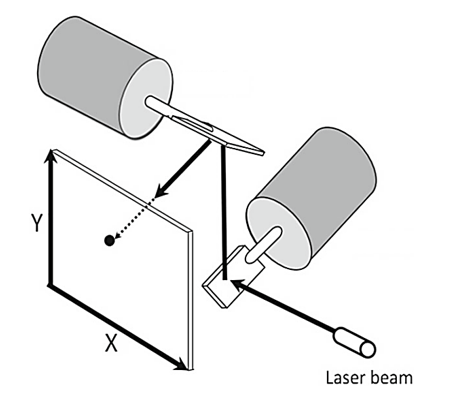
\includegraphics[width=0.5\textwidth]{figures/hardware_design/two_axis_scanner.png}
  \caption{Two-axis laser scanner schematic. This figure was modified from \cite{two-axis-scanner-schematic}.}
  \label{fig:two-axis-scanner-schematic}
\end{figure}

When a single axis of the laser turret is considered it can be seen that a right triangle is formed between the laser turret and the $xy$-plane mosquito enclosure as shown in \autoref{fig:mirror_angle}. Using the properties of a right triangle the laser beam angle $\theta$ required to shine the laser a distance $d$ relative to the origin of the laser can be calculated using
\begin{equation}
  \theta = \arctan{\left(\frac{d}{z}\right)}\,,
  \label{eq:mirror_angle}
\end{equation}
where $z$ is the distance between the turret and the back wall of the mosquito enclosure.
\begin{figure}[!htb]
  \centering
  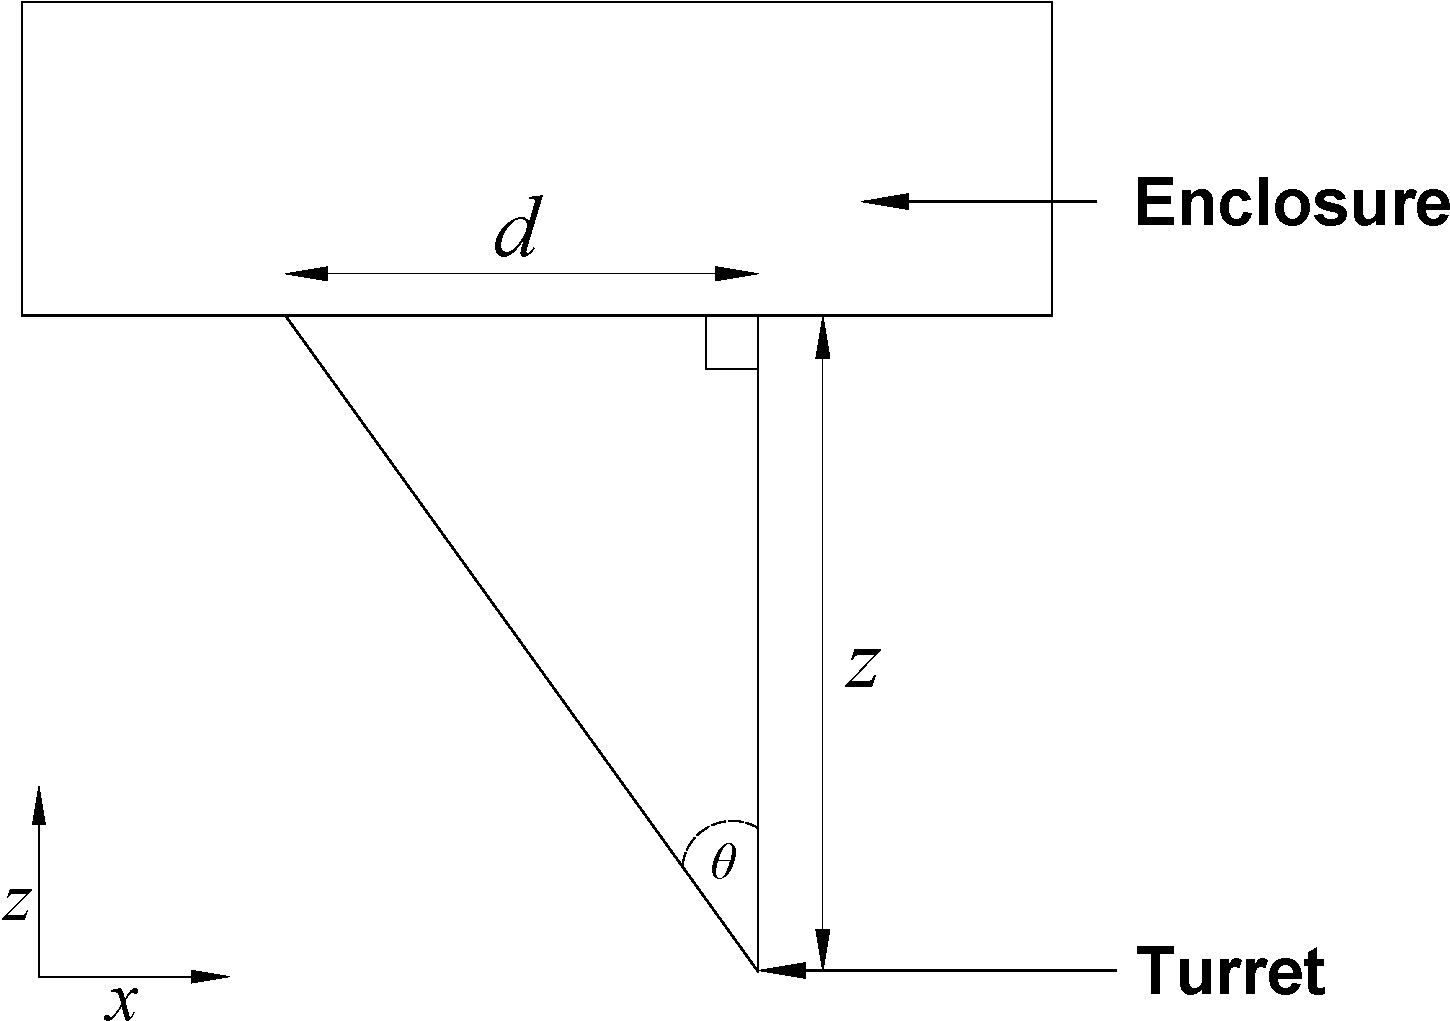
\includegraphics[width=0.6\textwidth]{figures/hardware_design/mirror_angle.pdf}
  \caption{The right triangle formed between the laser turret and the mosquito enclosure.}
  \label{fig:mirror_angle}
\end{figure}

\newcommand{\requiredLatStepSizeMM}{2}
The lateral step size of the laser must be a maximum of $d_{min} = \requiredLatStepSizeMM$\,mm. This will ensure that the laser will be able to illuminate every position in the mosquito enclosure since the laser itself will be a few millimetres wide.

\newcommand{\requiredLatSpeedMPS}{1}
The required lateral speed is determined in accordance with the field specifications. The longest length of the mosquito enclosure $d_{max}$ will be $\SI{1}{\meter}$. To ensure that the laser can illuminate any setpoint inside the mosquito enclosure within $\SI{2}{\second}$ of receiving a step input, it was assumed that the laser must be able to move with a velocity $v_{laser}$ of least $\SI{\requiredLatSpeedMPS}{\meter\per\second}$ opposed to the $\SI{0.5}{\meter\per\second}$ required to move the $\SI{1}{\meter}$ length of the mosquito enclosure within $\SI{2}{\second}$. This was done to accommodate for the settling time of the laser turret control system.




\FloatBarrier
\subsection{Hardware implementation}\label{subsec:hardware_implementation}
\subsubsection{Mosquito enclosure}
% \newcommand{\enclosureWidthCM}{100} % cm
\newcommand{\enclosureHeightCM}{38} % cm
% \newcommand{\enclosureDepthCM}{32} % cm
% The mosquito enclosure was constructed from a second hand glass fish tank with dimensions in the form $xyz$ given by $\enclosureWidthCM \times \enclosureHeightCM \times \enclosureDepthCM$ cm.
The mosquito enclosure was constructed from a second hand glass fish tank. All the surfaces other than front facing surface was retrofitted with a white lining. Internal \glspl{led} were added to the enclosure, shining from the top and bottom surfaces to minimise shadows on the back surface the enclosure, to ensure contrast between the background and the mosquitoes and to minimise the camera noise.



\subsubsection{System positioning}\label{subsubsec:system_positioning}
The laser turret and the camera was placed outside the mosquito enclosure in known positions relative to the enclosure. The bracket, shown in \autoref{fig:system_positioning_bracket}, was built to hold the laser turret and the camera in place relative to the mosquito enclosure. The laser turret and camera will be mounted on the bracket using 3D printed clamps.
\begin{figure}[!htb]
  \centering
  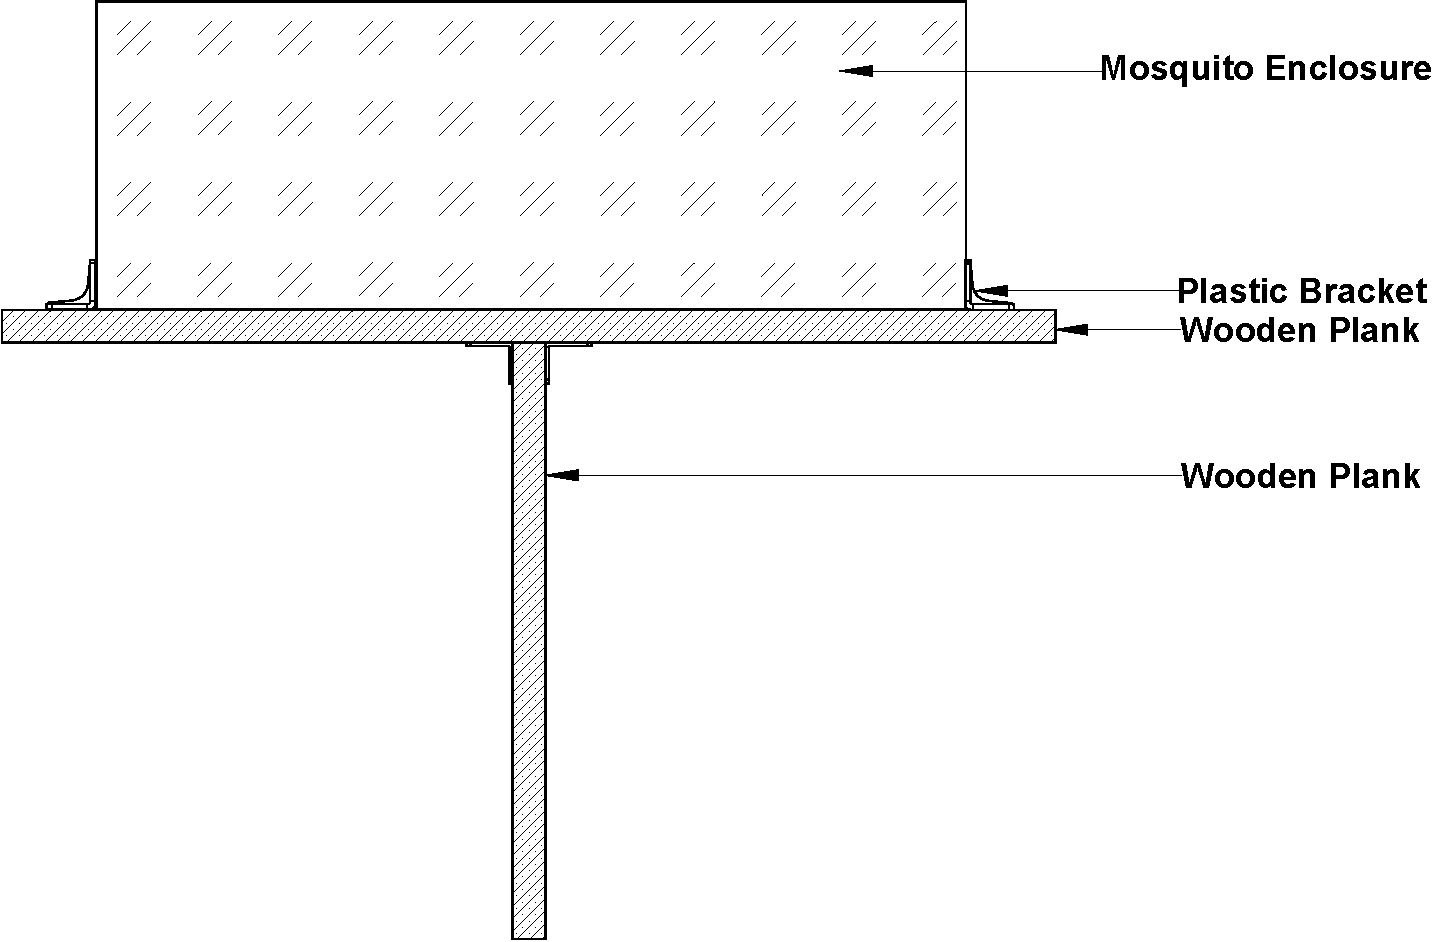
\includegraphics[width=0.85\textwidth]{figures/hardware_design/system_positioning.pdf}
  \caption{System positioning bracket.}
  \label{fig:system_positioning_bracket}
\end{figure}


\subsubsection{Camera mounting}
The camera was mounted on the bracket in \autoref{fig:system_positioning_bracket} using a 3D printed camera mount. The camera mount was designed to be adjustable to ensure that the camera can be positioned in the centre of the mosquito enclosure. The camera mounts were designed in \gls{cad}. The camera mount is shown in \autoref{fig:camera_mount_and_base_clamp}.
\begin{figure}[!htb]
  \centering
  \begin{subfigure}[b]{0.45\textwidth}
    \centering
    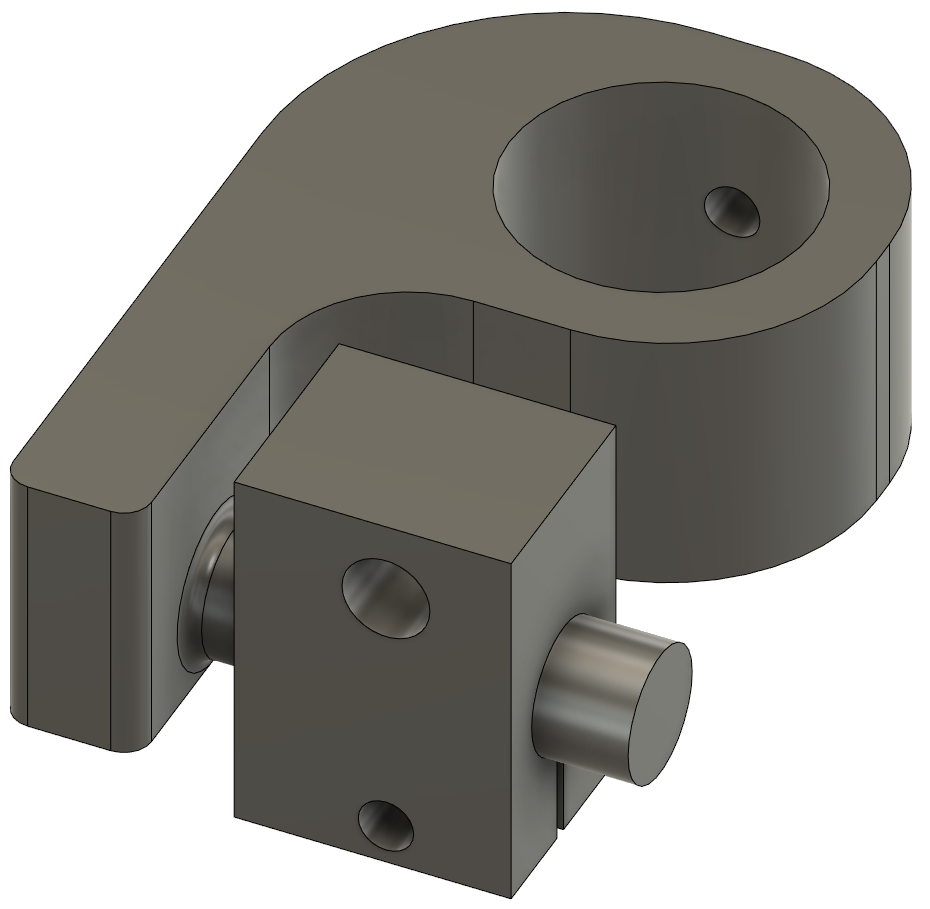
\includegraphics[width=0.7\linewidth]{figures/hardware_design/camera_and_middle_clamp.png}
    \caption{Camera mount.}
    \label{fig:camera_mount}
  \end{subfigure}
  \quad
  \begin{subfigure}[b]{0.45\textwidth}
    \centering
    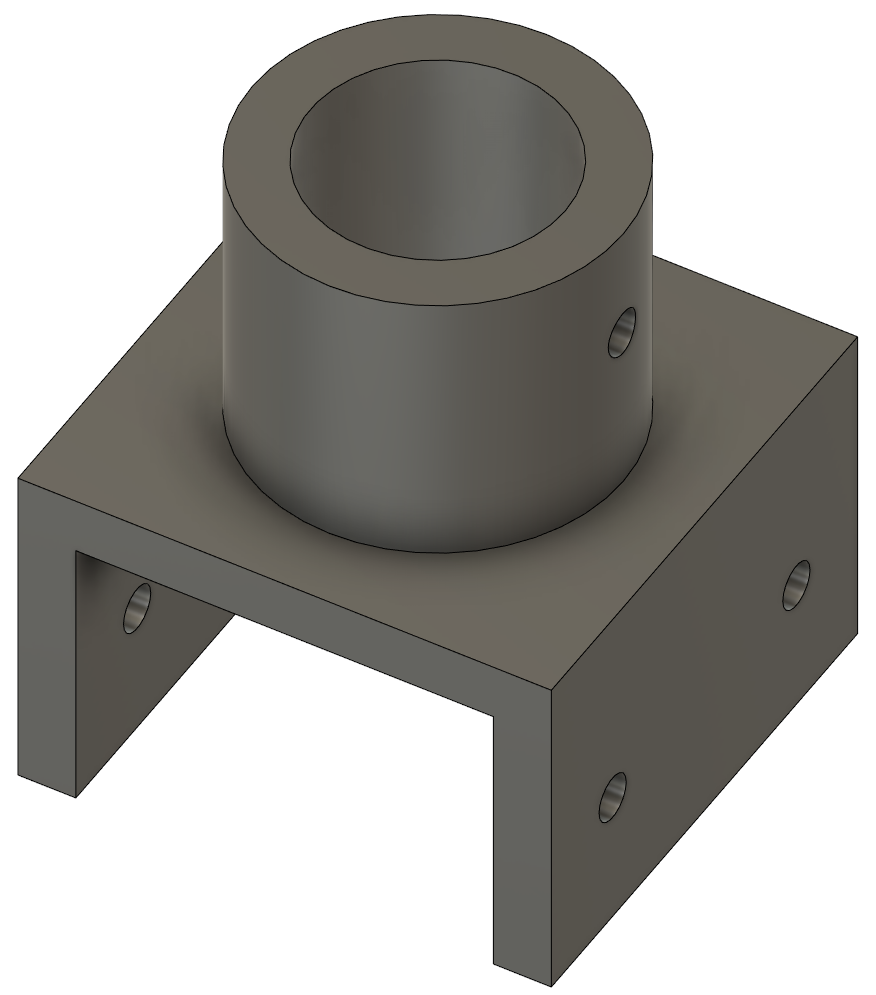
\includegraphics[width=0.7\linewidth]{figures/hardware_design/camera_base_clamp.png}
    \caption{Camera base clamp.}
    \label{fig:camera_base_clamp}
  \end{subfigure}
  \caption{The camera mount and camera base clamp.}
  \label{fig:camera_mount_and_base_clamp}
\end{figure}



\subsubsection{Laser turret}\label{subsubsec:laser_turret_design}
The specific geometry of the laser turret was designed with the goal to practically obtain a sufficiently small lateral step size of the laser on the back wall of the mosquito enclosure, while maintaining sufficient speed. The dimensions of the mirrors were chosen for practicality as $30 \times 15 \times 3$~mm.


\label{par:angular_step_size}
\paragraph{Angular step size}\mbox{}\\
The turret axis on which the laser beam is first incident on will be referred to as the first axis and the other axis will be referred to as the second axis for the remainder of this discussion. The rotation range of the first axis is bounded by the geometry of the turret since the laser beam reflected from the first axis must be incident on the second axis. With the chosen mirror dimensions, the maximum angle through which the first axis can rotate is $40\degree$, which rotates the laser beam through $80\degree$. This was determined geometrically in the scale drawing in \autoref{fig:turret_motion_range}. To accommodate for the mounting and alignment of the mirrors as well as other imperfections it was decided to consider a maximum rotation of $20\degree$, resulting in $\theta_{laser}^{max} = 40\degree$. The rotation range of the second axis is not bounded by the geometry of the laser turret since the laser beam reflected from the second axis is incident on the mosquito enclosure. Therefore, the laser turret will be oriented such that the first axis moves the laser beam parallel to the shorter height of the mosquito enclosure and the second axis moves the laser beam parallel to the longer width of the mosquito enclosure.
\begin{figure}[!htb]
  \centering
  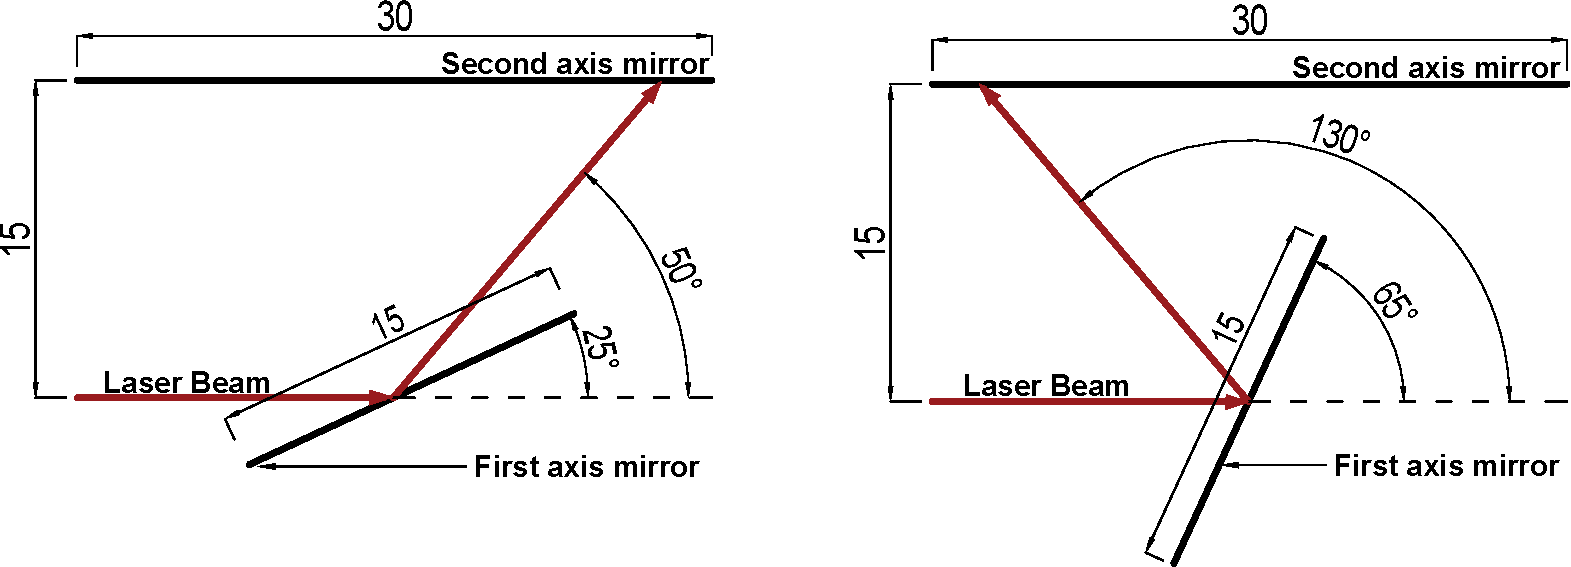
\includegraphics[width=\textwidth]{figures/anton hoeke.pdf}
  \caption{The rotation range of the first axis with chosen mirror dimensions.}
  \label{fig:turret_motion_range}
\end{figure}

The minimum distance $z_{min}$ between the laser turret and the mosquito enclosure can be determined by rearranging \autoref{eq:mirror_angle} to give
\FPeval{\zMinCM}{round(\enclosureHeightCM/tan(40*pi/180), 1)}
\begin{equation}
  z_{min} = \frac{d}{\tan\left(\theta_{laser}^{max}\right)} = \frac{\enclosureHeightCM\,\text{cm}}{\tan\left(40\degree\right)} = \zMinCM\,\text{cm}\,,
\end{equation}
where $d = \enclosureHeightCM$~cm is the height of the mosquito enclosure and $\theta_{laser}^{max} = 40\degree$ is the maximum angle through which the first axis of the laser can rotate. The maximum step resolution $\theta_{step}^{max}$ of the motors can be calculated by substituting $z_{min}$ and the required lateral step size $d_{min}$ into an equation derived from \autoref{eq:mirror_angle} given by
\pgfmathsetmacro{\stepRes}{atan2(\requiredLatStepSizeMM, \zMinCM*10)}
\begin{equation}
  \theta_{step}^{max} = \frac{1}{2}\arctan\left({\frac{d_{min}}{z_{min}}}\right) = \frac{1}{2}\arctan\left({\frac{\requiredLatStepSizeMM\,\text{mm}}{\zMinCM\,\text{cm}}}\right) = \frac{\FPeval{\roundStepRes}{round(\stepRes, 3)}\roundStepRes\degree}{2} = \FPeval{\roundStepRes}{round(\stepRes/2, 3)}\roundStepRes\degree\,.
  \label{eq:max_step_resolution}
\end{equation}
The division by two in \autoref{eq:max_step_resolution} is done to compensate for the fact the laser beam angle is double the mirror angle.

\paragraph{Angular speed}\mbox{}\\
The maximum angular speed $\omega_{max}$ required by the motors can be determined with $d_{max}=1$\,m, $v_{laser}=\SI{1}{\meter\per\second}$, and $z_{min}=\zMinCM$\,cm. The maximum angle through which the turret must rotate is
\begin{equation}
  \theta_{motor}^{max} = \frac{1}{2}\arctan\left({\frac{d_{max}}{z_{min}}}\right) = \frac{1}{2}\arctan\left({\frac{\SI{1}{\meter}}{\zMinCM\,\text{cm}}}\right) = \frac{65.6\degree}{2} = 32.8\degree\,.
\end{equation}
The maximum angular speed required to move the laser beam at the lateral speed $v_{laser} = \SI{\requiredLatSpeedMPS}{\meter\per\second}$ is
\begin{equation}
  \omega_{max} = v_{laser} \times \theta_{motor}^{max} = \SI{32.8}{\degree\per\second} = \SI{0.572}{\radian\per\second}\,.
\end{equation}
The results in a required motor \gls{rpm} of
\begin{equation}
  \omega_{max} = \SI{0.572}{\radian\per\second} \times \frac{60}{2\pi} = 5.5\,\text{RPM}\,.
\end{equation}


\paragraph{Torque}\hfill\\
The required torque $\tau$ was calculated using
\begin{equation}
  \tau = I\alpha\,,
  \label{eq:torque}
\end{equation}
where $I$ is the moment of inertia of the load, which is the mirror, and $\alpha$ is the required angular acceleration.

\begin{figure}[!htb]
  \centering
  % 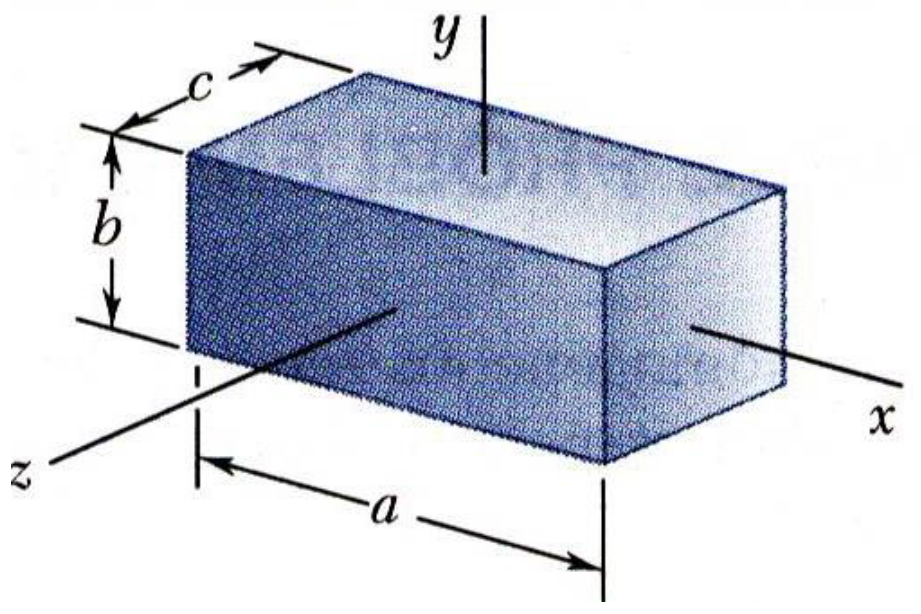
\includegraphics[width=0.5\textwidth]{figures/hardware_design/rect_inertia.png}
  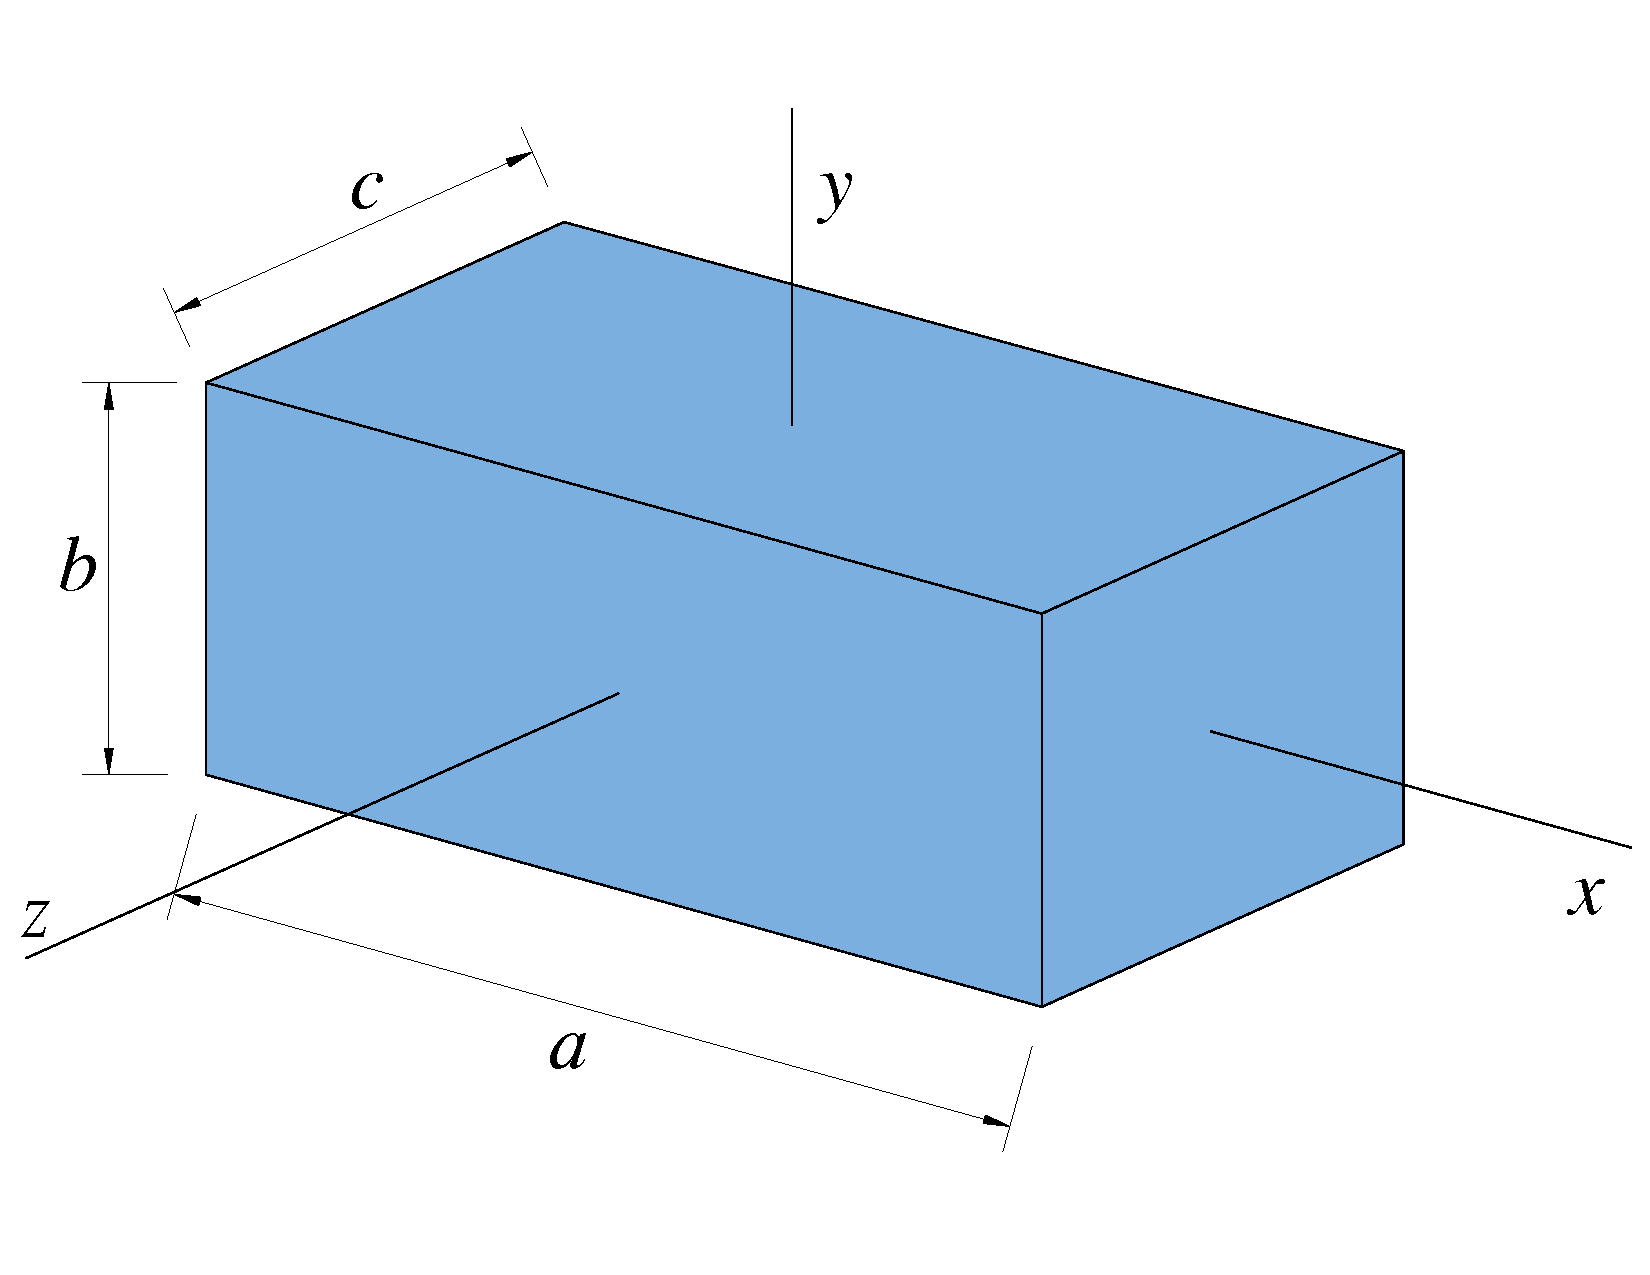
\includegraphics[width=0.6\textwidth]{figures/hardware_design/inertia_of_rectangle.pdf}
  \caption{Axes and dimensions of a rectangular prism.}
  \label{fig:rect_inertia}
\end{figure}
The moment of inertia of the mirror was calculated using the equation for the moment of inertia of a rectangular prism with rotation about its $x$-axis as seen in \autoref{fig:rect_inertia} given by
\begin{equation}
  I = \frac{1}{12}M\left(b^2 + c^2\right)\,,
\end{equation}
where $M$ is the mass of the rectangular prism and $b$ and $c$ are the dimensions of the rectangular prism. The mass of the rectangular prism $M$ will be calculated using the density of glass $\rho = \SI{2500}{\kg\per\meter\cubed}$ and the volume of the rectangular prism $V$ given by
\begin{equation}
  V = abc\,,
\end{equation}
where $a$, $b$, and $c$ are the dimensions of the rectangular prism. The dimensions of the rectangular prism are given by the chosen mirror dimensions as $a = 30\,\text{mm}$, $b = 15\,\text{mm}$, and $c = 3\,\text{mm}$. The mass of the mirror $M$ is
\begin{equation}
  M = \rho V = \SI{2500}{\kg\per\meter\cubed} \times (30\,\text{mm})(15\,\text{mm})(3\,\text{mm}) = 3.38\,\text{g}\,.
\end{equation}
Thus, the moment of inertia of the mirror is
\begin{equation}
  I = \frac{1}{12}M\left(b^2 + c^2\right) = \frac{1}{12}(3.38\,\text{g})\left((15\,\text{mm})^2 + (3\,\text{mm})^2\right) = \SI{6.59e-8}{\kg\per\meter\squared}\,.
\end{equation}

The required angular acceleration of the motor $\alpha$ is calculated with
\begin{equation}
  \alpha = \frac{\Delta\omega}{\Delta t}\,,
\end{equation}
where $\Delta\omega = \omega_{max} - 0$ is the change in angular velocity and $\Delta t$ is the change in time. The change in time $\Delta t$ was determined by assuming the laser must be able to accelerate from a stand still to $v_{laser} = \SI{1}{\meter\per\second}$ extremely rapidly to ensure that the motors could respond to the irregular flight pattern of a mosquito. It was assumed that this acceleration must occur within 10~ms. Thus, the required angular acceleration $\alpha$ is
\begin{equation}
  \alpha = \frac{\Delta\omega}{\Delta t} = \frac{\SI{0.572}{\radian\per\second}}{\SI{0.01}{\second}} = \SI{57.2}{\radian\per\second\squared}\,.
\end{equation}

Given the calculated moment of inertia and angular acceleration the required torque $\tau$ is
\begin{equation}
  \tau = I\alpha = \SI{6.59e-8}{\kg\per\meter\squared} \times \SI{57.2}{\radian\per\second\squared} = \SI{3.77e-6}{\newton\meter}\,.
\end{equation}


\paragraph{Motor and driver selection}\hfill\\
Typical stepper motors have a basic step angle of $1.8\degree$. This does not meet the required step resolution $\theta_{step}^{max} = 0.253\degree$, however the step angle can be reduced by using microstepping. Microstepping works by interpolating the \gls{pwm} signal to the stepper motor driver to produce intermediate step positions between the basic step positions. Stepper motor drivers that support up to 16 microsteps are readily available. Drivers that support up to 256 microsteps are also available. The step angle $\theta_{step}$ of a stepper motor using 16 microsteps is
\begin{equation}
  \theta_{step} = \frac{1.8\degree}{16} = 0.1125\degree\,,
\end{equation}
which is sufficient to meet the required maximum step resolution $\theta_{step}^{max} = 0.127\degree$. Therefore, a typical stepper motor with a basic step angle of $1.8\degree$ operated using at least 16 microsteps will be sufficient.

A drawback of using microstepping is that the effective torque of the stepper motor is reduced with each increase in microstepping. The torque reduction due to microstepping can be calculated with
\begin{equation}
  \tau_{eff} = \tau_{rated} \sin \left(\frac{\pi S}{2}\right)\,,
\end{equation}
where
\begin{itemize}
  \item $\tau_{eff}$ is the effective torque of the stepper motor for a specific amount of microstepping.
  \item $\tau_{rated}$ is the rated torque of the stepper motor.
  \item $S$ is the reciprocal of the number of microsteps.
\end{itemize}

The effective torque of a stepper motor for the full range of microsteps available is tabulated in \autoref{tab:effective_torque}. It can be seen that microstepping has a drastic impact on the effective torque of stepper motors. Thus, the required torque will need to be calculated for the chosen microstepping operation.
\begin{table}[!htb]
  \centering
  \begin{tabular}{|c|c|}
    \hline
    Microsteps & Effective torque \\
    \hline
    1          & 100\%            \\
    2          & 70.71\%          \\
    4          & 38.27\%          \\
    8          & 19.51\%          \\
    16         & 9.8\%            \\
    32         & 4.91\%           \\
    64         & 2.45\%           \\
    128        & 1.23\%           \\
    256        & 0.61\%           \\
    \hline
  \end{tabular}
  \caption{Effective torque of stepper motor for full range of microsteps.}
  \label{tab:effective_torque}
\end{table}

The DRV8825 stepper motor driver was chosen since it is readily available and supports up to 32 microsteps. The DRV8825 stepper motor driver has a maximum current rating of 2.5~A and a maximum voltage rating of 45~V. The maximum microstepping mode will be utilised for increased resolution in the control of the laser. The required torque with 32 microsteps is
\begin{equation}
  \tau_{required} = \SI{3.77e-6}{\newton\meter} \times \frac{100\%}{4.91\%} = \SI{7.68e-5}{\newton\meter}\,.
\end{equation}

A bipolar NEMA8 stepper motor with specifications shown in \autoref{tab:nema8_specs}
\begin{table}[!htb]
  \centering
  \begin{tabular}{rl}
    \hline
    Basic step angle & $\SI{1.8}{\degree}$                               \\
    Holding torque   & $180\,\text{g\,cm} = \SI{1.77e-2}{\newton\meter}$ \\
    Rated voltage    & 3.9~V                                             \\
    Rated current    & 0.6~A                                             \\
    \hline
  \end{tabular}
  \caption{Specifications of the NEMA8 stepper motor.}
  \label{tab:nema8_specs}
\end{table}
\begin{figure}[!htb]
  \centering
  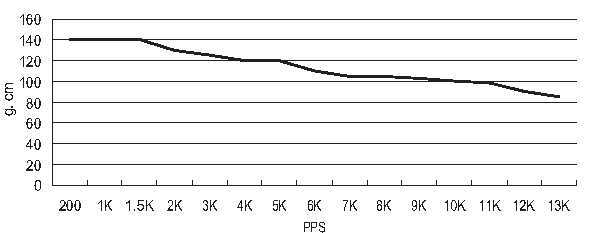
\includegraphics[width=\textwidth]{figures/hardware_design/torque_curve.pdf}
  \caption{Pull-out torque curve of the stepper motor at half step with 24~V and 0.6~A.}
  \label{fig:torque_curve}
\end{figure}
and a pull-out torque curve at half step shown in \autoref{fig:torque_curve} was chosen as the motors for the laser turret. From the pull-out torque curve in \autoref{fig:torque_curve}, the maximum rated speed of the motor is given as 13\,000 points per second at half step $0.9\degree$ which is
\begin{equation}
  \num{13000} \div \frac{360\degree}{0.9\degree} = 32.5\,\text{RPM}\,,
\end{equation}
with a pull-out torque greater than 100\,g\,cm = $\SI{9.8e-3}{\newton\meter}
$. The effective torque of the stepper motor at maximum speed with 32 microsteps is
\begin{equation}
  \tau_{eff} = \SI{9.8e-3}{\newton\meter} \times 4.91\% = \SI{4.81e-4}{\newton\meter}\,.
\end{equation}
The effective torque of the stepper motor at maximum speed is greater than the required torque for the laser turret, therefore the NEMA8 stepper motor is suitable for the laser turret and was also chosen for its compactness which can be seen in \autoref{fig:nema8_dimensions}.
\begin{figure}[!htb]
  \centering
  \begin{subfigure}{0.45\textwidth}
    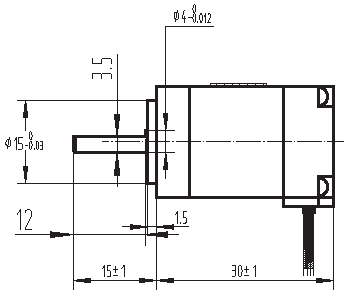
\includegraphics[width=\linewidth]{figures/hardware_design/nema8_side_view.pdf}
    \caption{Side view.}
  \end{subfigure}
  \quad
  \begin{subfigure}{0.45\textwidth}
    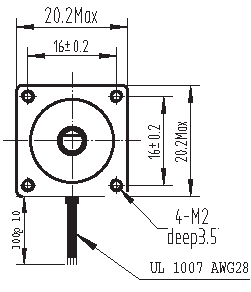
\includegraphics[width=0.75\linewidth]{figures/hardware_design/nema8_front_view.pdf}
    \caption{Front view.}
  \end{subfigure}
  \caption{Dimensions of the NEMA8 stepper motor.}
  \label{fig:nema8_dimensions}
\end{figure}


\paragraph{Laser selection and activation circuit}\label{par:laser_activation}\hfill\\
A low-powered 5\,mW red laser with adjustable focus was chosen for the laser turret. The laser has an operating voltage range of $2.8 - 5.2$\,V. A low-powered laser was chosen for safety. The adjustable focus enabled the laser beam to be focused to a small area on the back wall of the mosquito enclosure. The laser must be red since the image processing will be done using only the red channel of the \gls{rgb} video frame.

The 3.3\,V \gls{gpio} of the Nvidia Jetson Nano cannot supply enough current to power the laser. A switching transistor circuit was designed to enable the laser to be turned on and off from the Nvidia Jetson Nano \gls{gpio}. The schematic for the switching transistor circuit can be seen in \autoref{fig:transistor_schematic}.  When the input signal is high the transistor is switched on and the laser is powered. When the input signal is low the transistor is switched off and the laser is not powered. In \autoref{fig:transistor_schematic}, $R1$ is a pull-down resistor to ensure that the input signal is low when the Nvidia Jetson Nano is not driving the input signal. $R1$ was chosen as $56\,k\Omega$ to limit the current drawn from the Nvidia Jetson Nano \gls{gpio}. With $R1 = 56\,k\Omega$ the current drawn from the \gls{gpio} is $\frac{3.3\,V}{56\,k\Omega} = 59\,\mu A$. $R2$ and $D1$ represent the laser.
\begin{figure}[!htb]
  \centering
  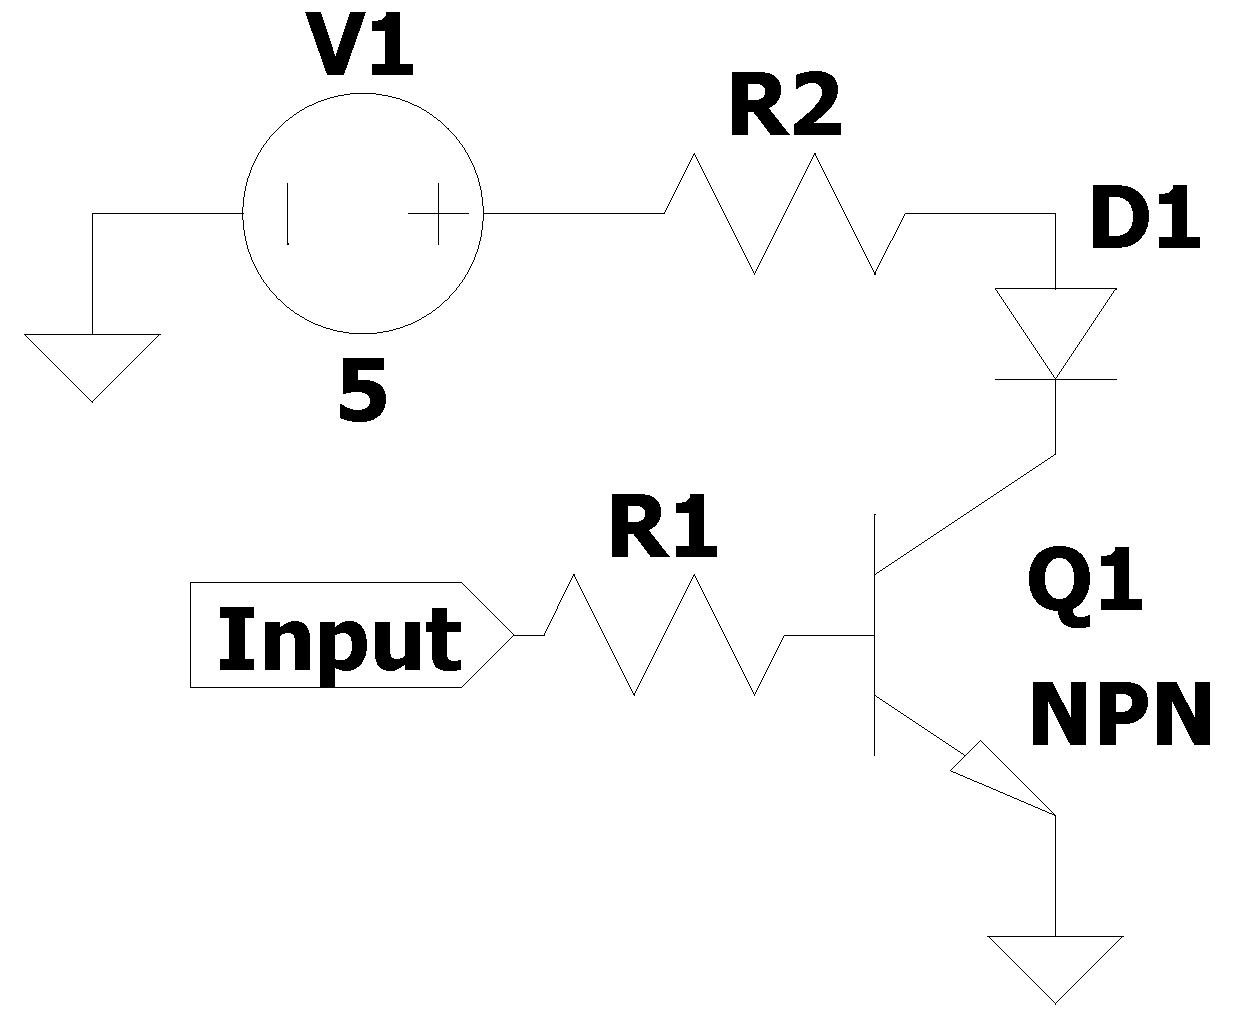
\includegraphics[width=0.45\textwidth]{figures/hardware_design/laser_transistor_schematic.pdf}
  \caption{Switching transistor circuit.}
  \label{fig:transistor_schematic}
\end{figure}


\paragraph{Laser turret \gls{cad}}
The laser turret was designed in \gls{cad} using Autodesk Fusion 360. The laser turret was designed to be mounted on the bracket shown in \autoref{fig:system_positioning_bracket}. The main component and subcomponents of the laser turret can be seen in \autoref{fig:turret_cad} and \autoref{fig:turret_subcomponents} respectively.
\begin{figure}[!htb]
  \centering
  \begin{subfigure}[t]{0.45\textwidth}
    \centering
    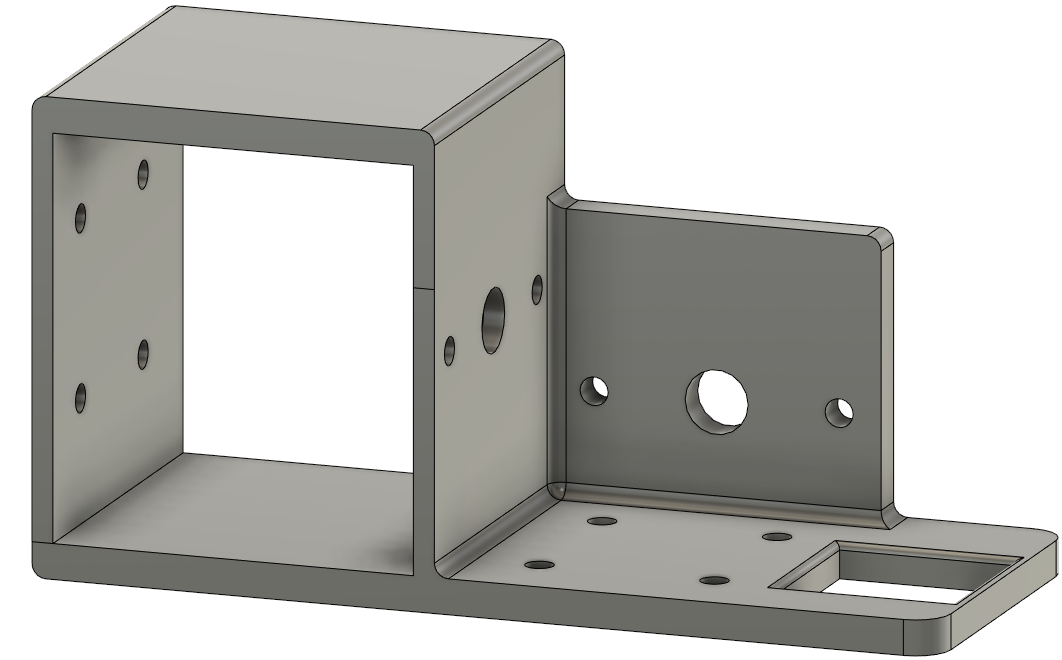
\includegraphics[width=\linewidth]{figures/hardware_design/turret_cad_90.png}
    \caption{Laser turret main housing.}
  \end{subfigure}
  \hfill
  \begin{subfigure}[t]{0.45\textwidth}
    \centering
    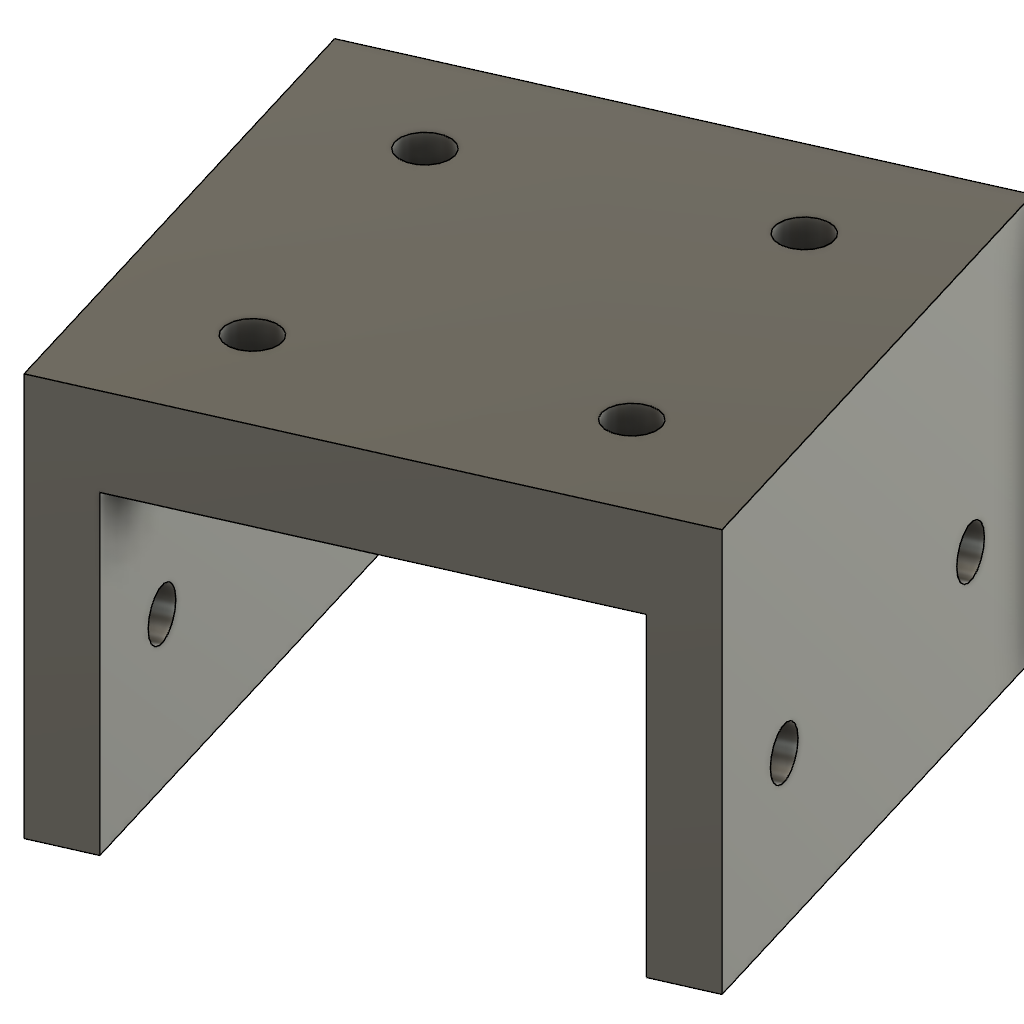
\includegraphics[width=0.55\linewidth]{figures/hardware_design/turret_clamp.png}
    \caption{Laser turret clamp.}
  \end{subfigure}
  \caption{Laser turret main components.}
  \label{fig:turret_cad}
\end{figure}
\begin{figure}[!htb]
  \centering
  \begin{subfigure}{0.3\textwidth}
    \centering
    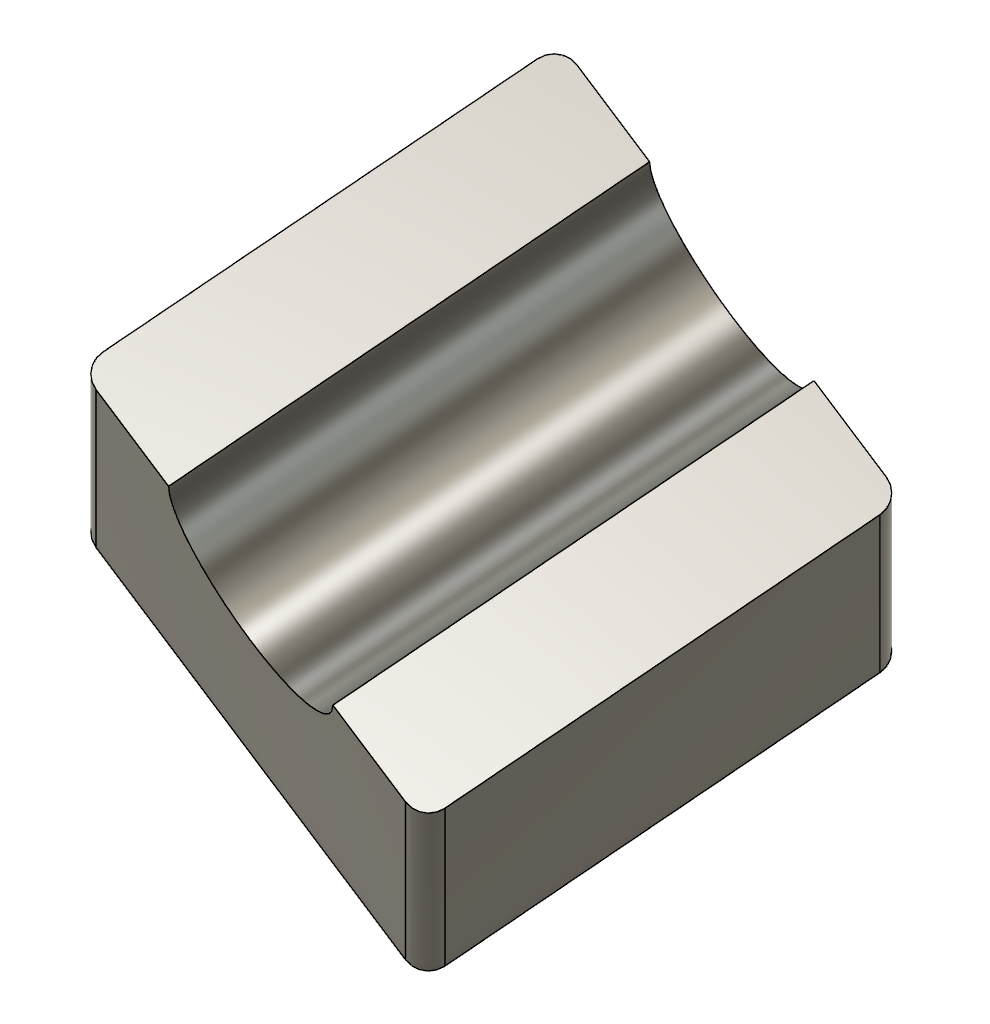
\includegraphics[width=0.7\linewidth]{figures/hardware_design/laser_mount.png}
    \caption{Laser mount.}
  \end{subfigure}
  \quad
  \begin{subfigure}{0.3\textwidth}
    \centering
    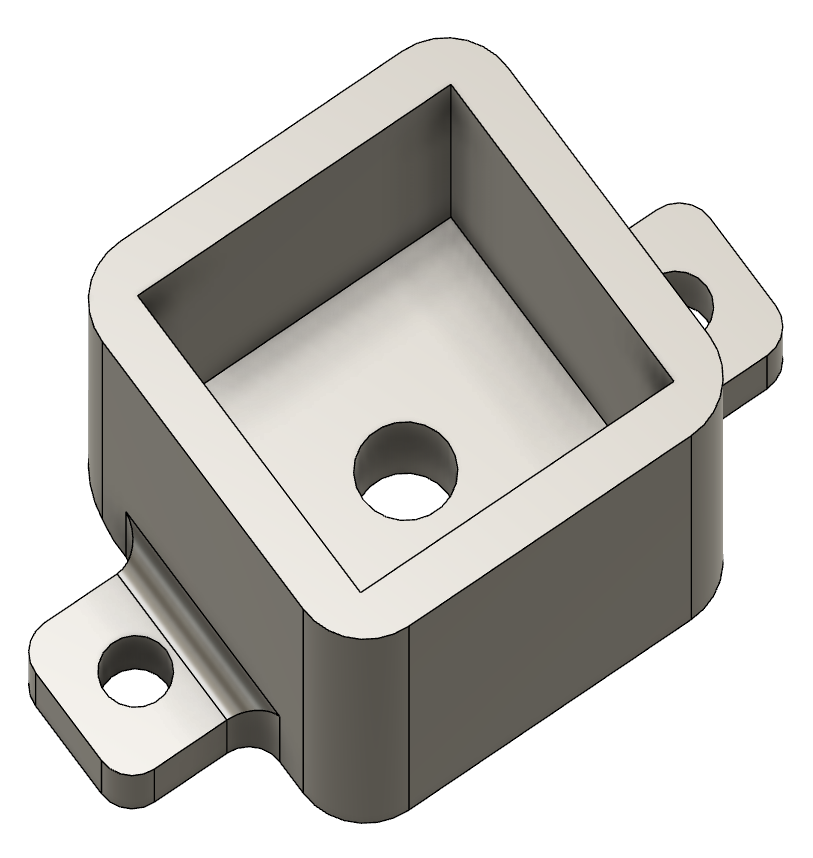
\includegraphics[width=0.7\linewidth]{figures/hardware_design/motor_mount.png}
    \caption{Motor mount.}
  \end{subfigure}
  \quad
  \begin{subfigure}{0.3\textwidth}
    \centering
    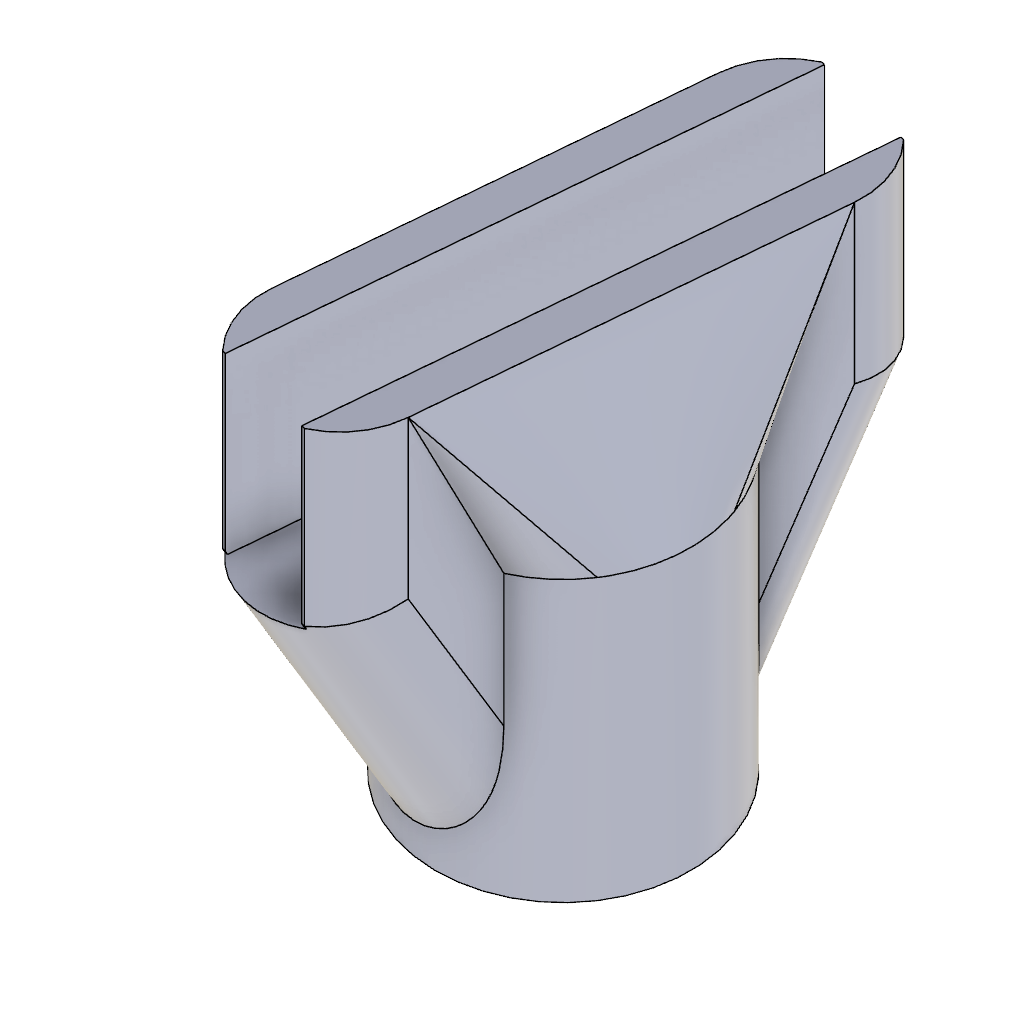
\includegraphics[width=0.7\linewidth]{figures/hardware_design/mirror_holder.png}
    \caption{Mirror holder.}
  \end{subfigure}
  \caption{Laser turret subcomponents.}
  \label{fig:turret_subcomponents}
\end{figure}


\subsubsection{Final system assembly}
The final assembly of the full system can be seen in \autoref{fig:side_view}.
The laser turret and camera configuration can be seen up close in \autoref{fig:turret_and_camera}.
\begin{figure}[!htb]
  \centering
  \includegraphics[width=0.8\textwidth]{figures/fotos/naas_side_view.png}
  \caption{The full system assembly.}
  \label{fig:side_view}
\end{figure}
\begin{figure}[!htb]
  \centering
  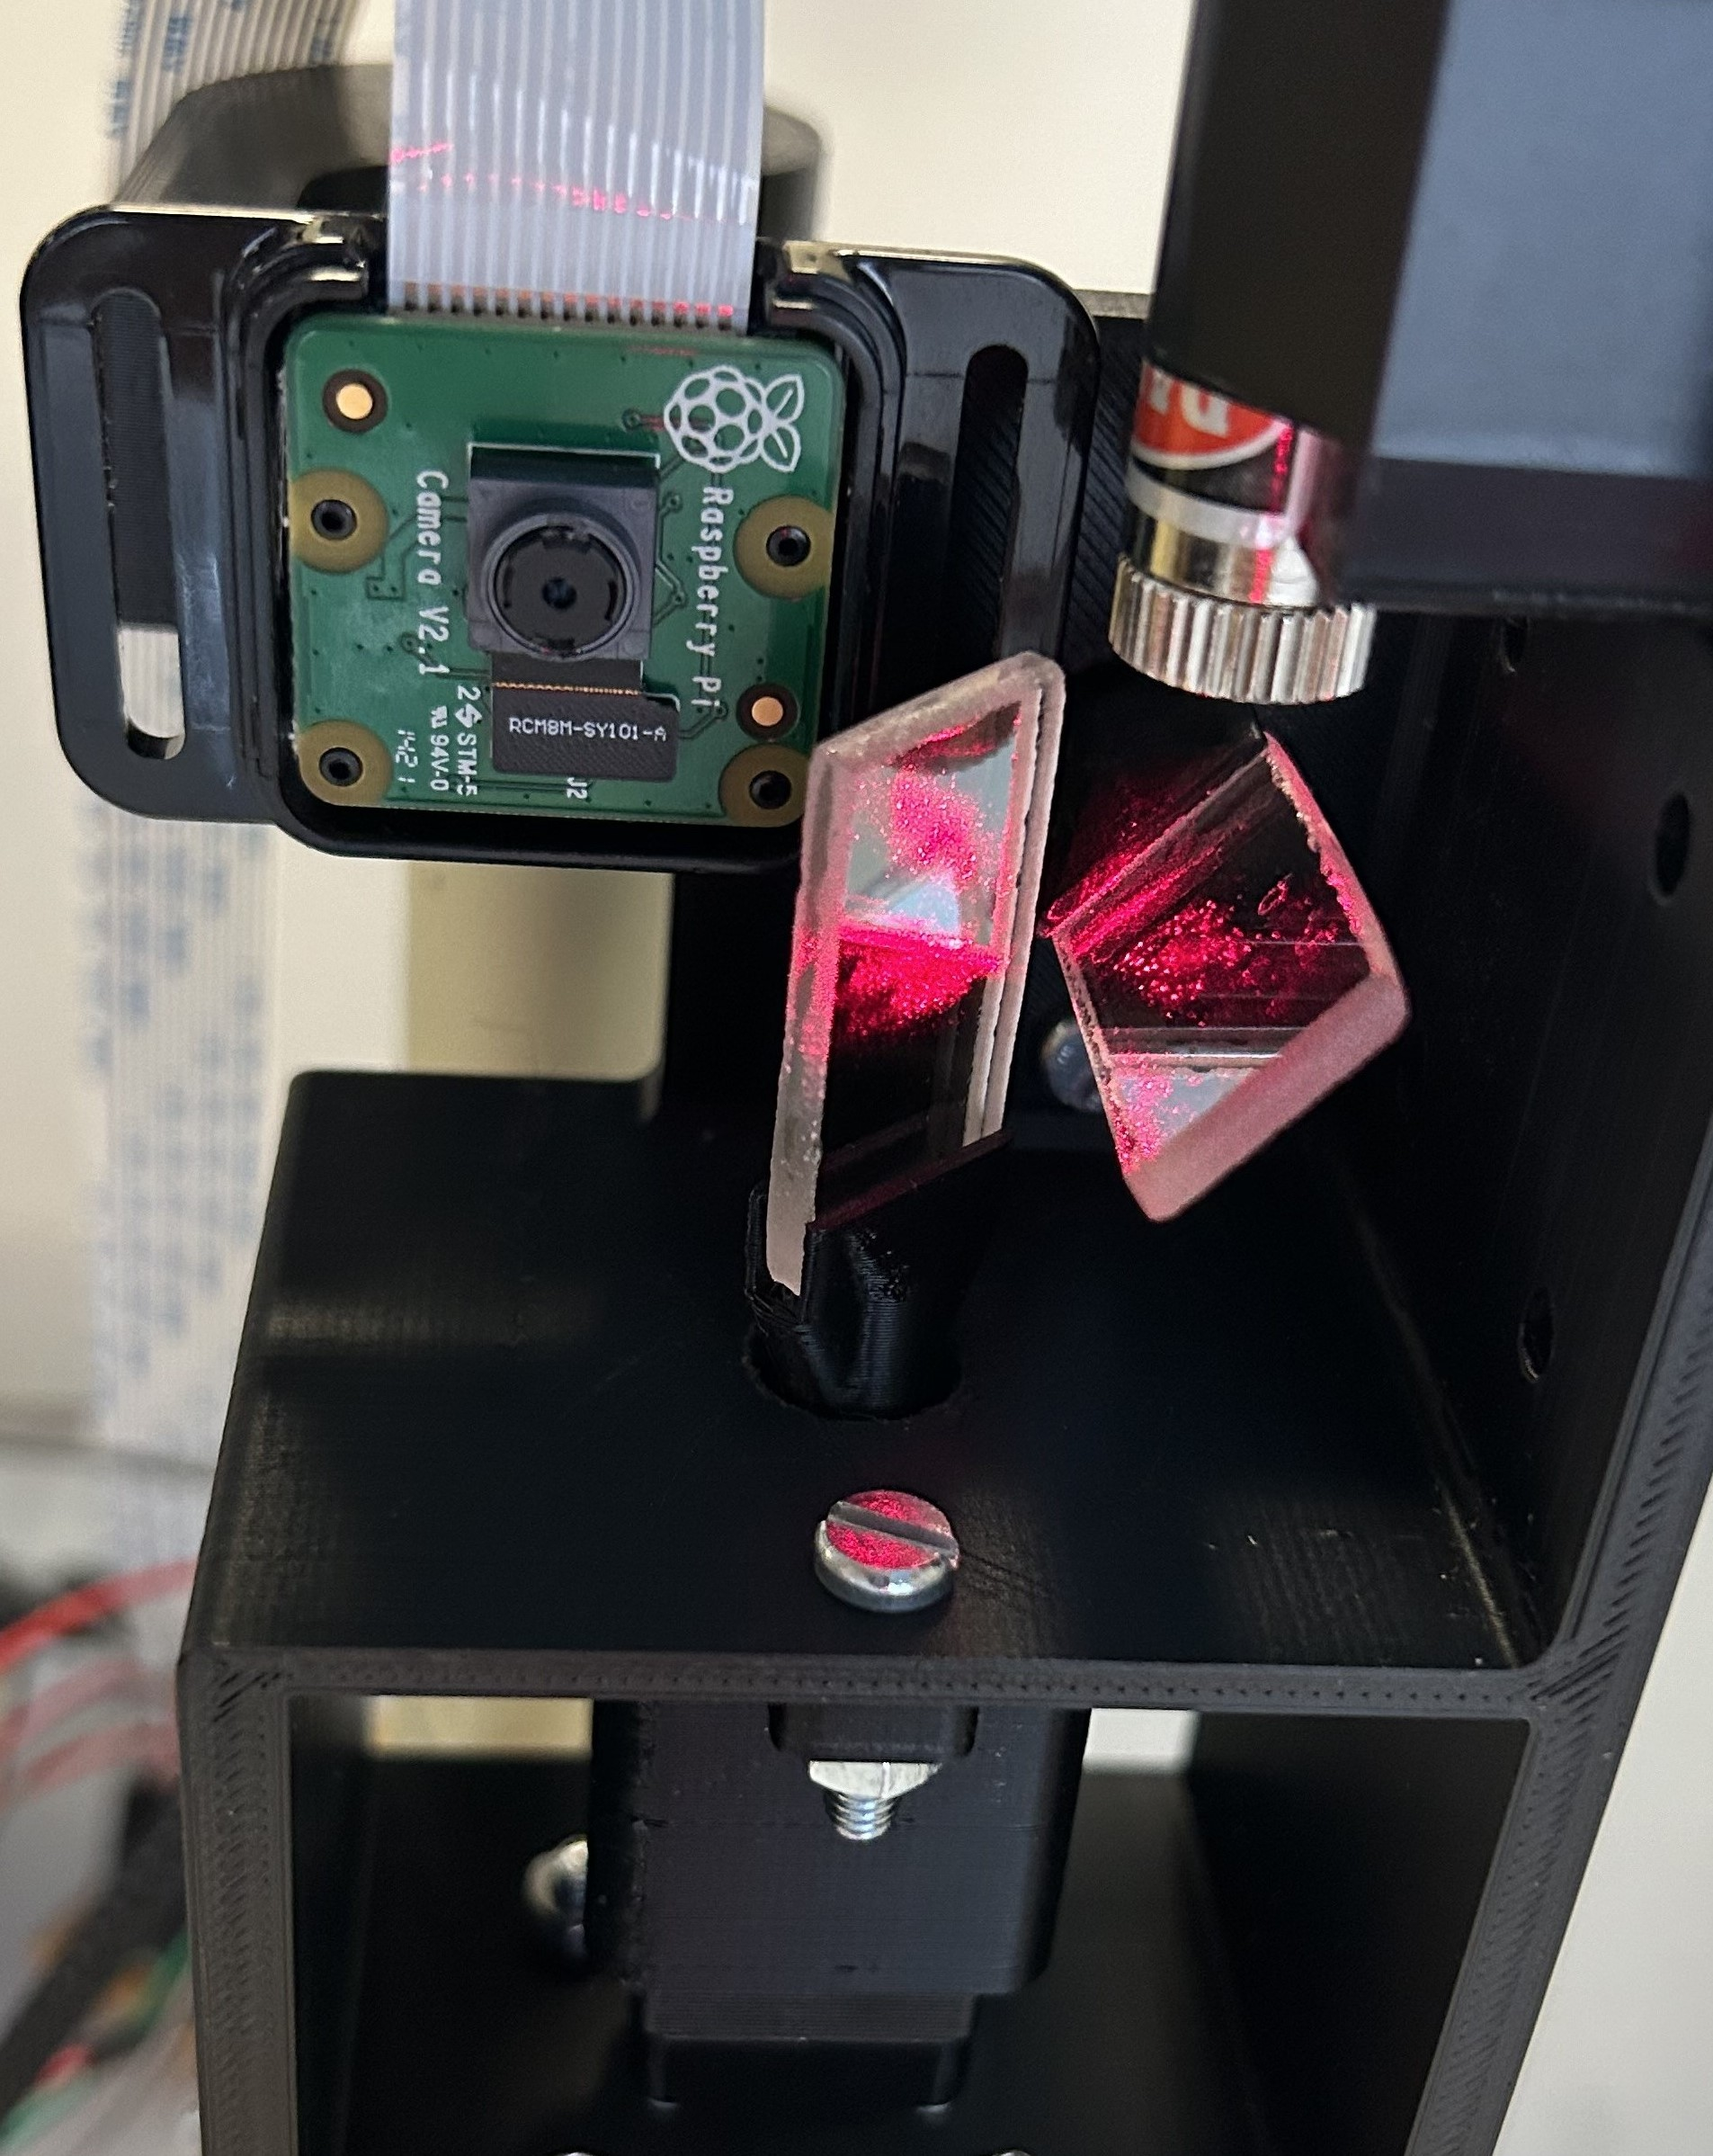
\includegraphics[width=0.43\textwidth]{figures/fotos/turret_and_camera_cropped.jpg}
  \caption{The laser turret and camera configuration.}
  \label{fig:turret_and_camera}
\end{figure}


\FloatBarrier
\subsection{Software design}\label{subsec:software_design}
\subsubsection{Mosquito and laser detection} \label{subsubsec:mosquito_and_laser_detection}
It was assumed that the mosquitoes would be the only dark blobs in the enclosure and that the laser's reflections would be the only bright blobs in the enclosure. The video frame will be cropped such that only the white back surface of the enclosure is visible. To reduce the computational complexity of the image processing only the red channel of the \gls{rgb} frame will be used, hence, the necessity of the red laser.

The mosquito detection was designed to detect dark blobs in the enclosure and would not be able to distinguish between mosquitoes and other dark blobs. The laser detection was designed to detect bright blobs in the enclosure and would not be able to distinguish between the laser's reflections and other bright blobs. The mosquito and laser detection processes are similar in nature. The basic detection process flow is shown in \autoref{fig:detection_process_flow}.
\begin{figure}[!htb]
  \centering
  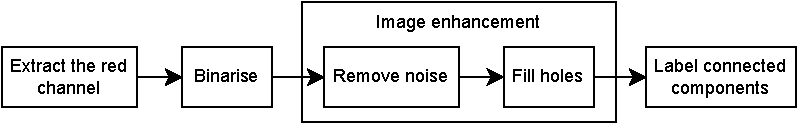
\includegraphics[width=\textwidth]{figures/detection/detection_process_flow.pdf}
  \caption{Detection process flow.}
  \label{fig:detection_process_flow}
\end{figure}
The red channel of the \gls{rgb} frame will be extracted, which will be referred to as the frame for the rest of this discussion. The difference between the mosquito and laser detection processes occur in the binarisation step. A copy of the frame is made before binarising so that both the mosquito and laser detection can be performed since the frame will be overwritten in the image processing steps in pursuit of efficiency.


\paragraph{Binarisation}\mbox{}\\
The frame will be binarised using a threshold value. The exposure of the camera will be fixed and the lighting in the mosquito enclosure will be controlled, thus the threshold value will be fixed. To detect mosquitoes the frame will be binarised with a less than threshold since the mosquitoes will be darker than the white background. To detect the laser's reflections the frame will be binarised with a greater than threshold since the laser and its reflections will be brighter than the white background. The ideal result of the binarisation is an image where the mosquitoes and the laser's reflections are the only foreground pixels in their respective copies of the frame. This will not be the case since the mosquitoes and the laser's reflections can not be perfectly isolated using a threshold value since the frame will contain noise from the camera sensor.


\paragraph{Image enhancement}\mbox{}\\
The binarised frames are subject to noise, holes, and erroneously joint or disjointed sections. This can be resolved using morphological operations.
The goal of the morphological operations is to ensure that all the foreground pixels that correspond to a detection are connected, that there are no foreground pixels that do not correspond to a detection, and that there are no erroneously joint or disjoint foreground pixels. There must be a one to one correspondence between the groups of connected foreground pixels and the objects that must be detected. The connectivity of pixels will be explained in \autoref{par:ccl}. Morphological operations work by passing a structuring element over the pixels in an image and performing a logical operation on the pixels in the image that are covered by the structuring element.

The noise and erroneously joint sections are removed using the morphological opening operation. Opening has been formally defined in \autoref{subsubsec:morphological_operations}. The opening of $A$ by $B$ is the union of all translations of $B$ that are completely contained in $A$ as illustrated in \autoref{fig:opening}. The holes and erroneously disjointed sections are removed using the morphological closing operation. Closing has been formally defined \autoref{subsubsec:morphological_operations}. The closing of $A$ by $B$ is the complement of the union of all translations of $B$ that do not overlap $A$ as illustrated in \autoref{fig:closing}.

The structuring element must be identical, independent of orientation, in a 2D image since the orientation of the mosquitoes will be unknown. The structuring element will therefore be a disc. The size of the disc will be adjusted independently for the opening and closing operations for both the mosquito and laser detection. The structuring elements' size will be adjustable at runtime such that they can be tuned to provide optimal performance.


\paragraph{Connected components labelling}\label{par:ccl}\mbox{}\\
From the enhanced binary frames the co-ordinates of the connected foreground pixels must be obtained. This is done using \gls{ccl}. \Gls{ccl} is the process of assigning a label to each foreground pixel in a binary image such that connected pixels have the same label. The connectivity of pixels are defined using either four or eight connectivity. Four connectivity defines the neighbourhood of a pixel as the pixels to the left, right, top, and bottom of the pixel. Eight connectivity defines the neighbourhood of a pixel as the pixels to the left, right, top, bottom, top left, top right, bottom left, and bottom right of the pixel. The \gls{ccl} connectivity is shown in \autoref{fig:ccl_connectivity}.
\begin{figure}[!htb]
  \centering
  \begin{subfigure}[b]{0.3\textwidth}
    \centering
    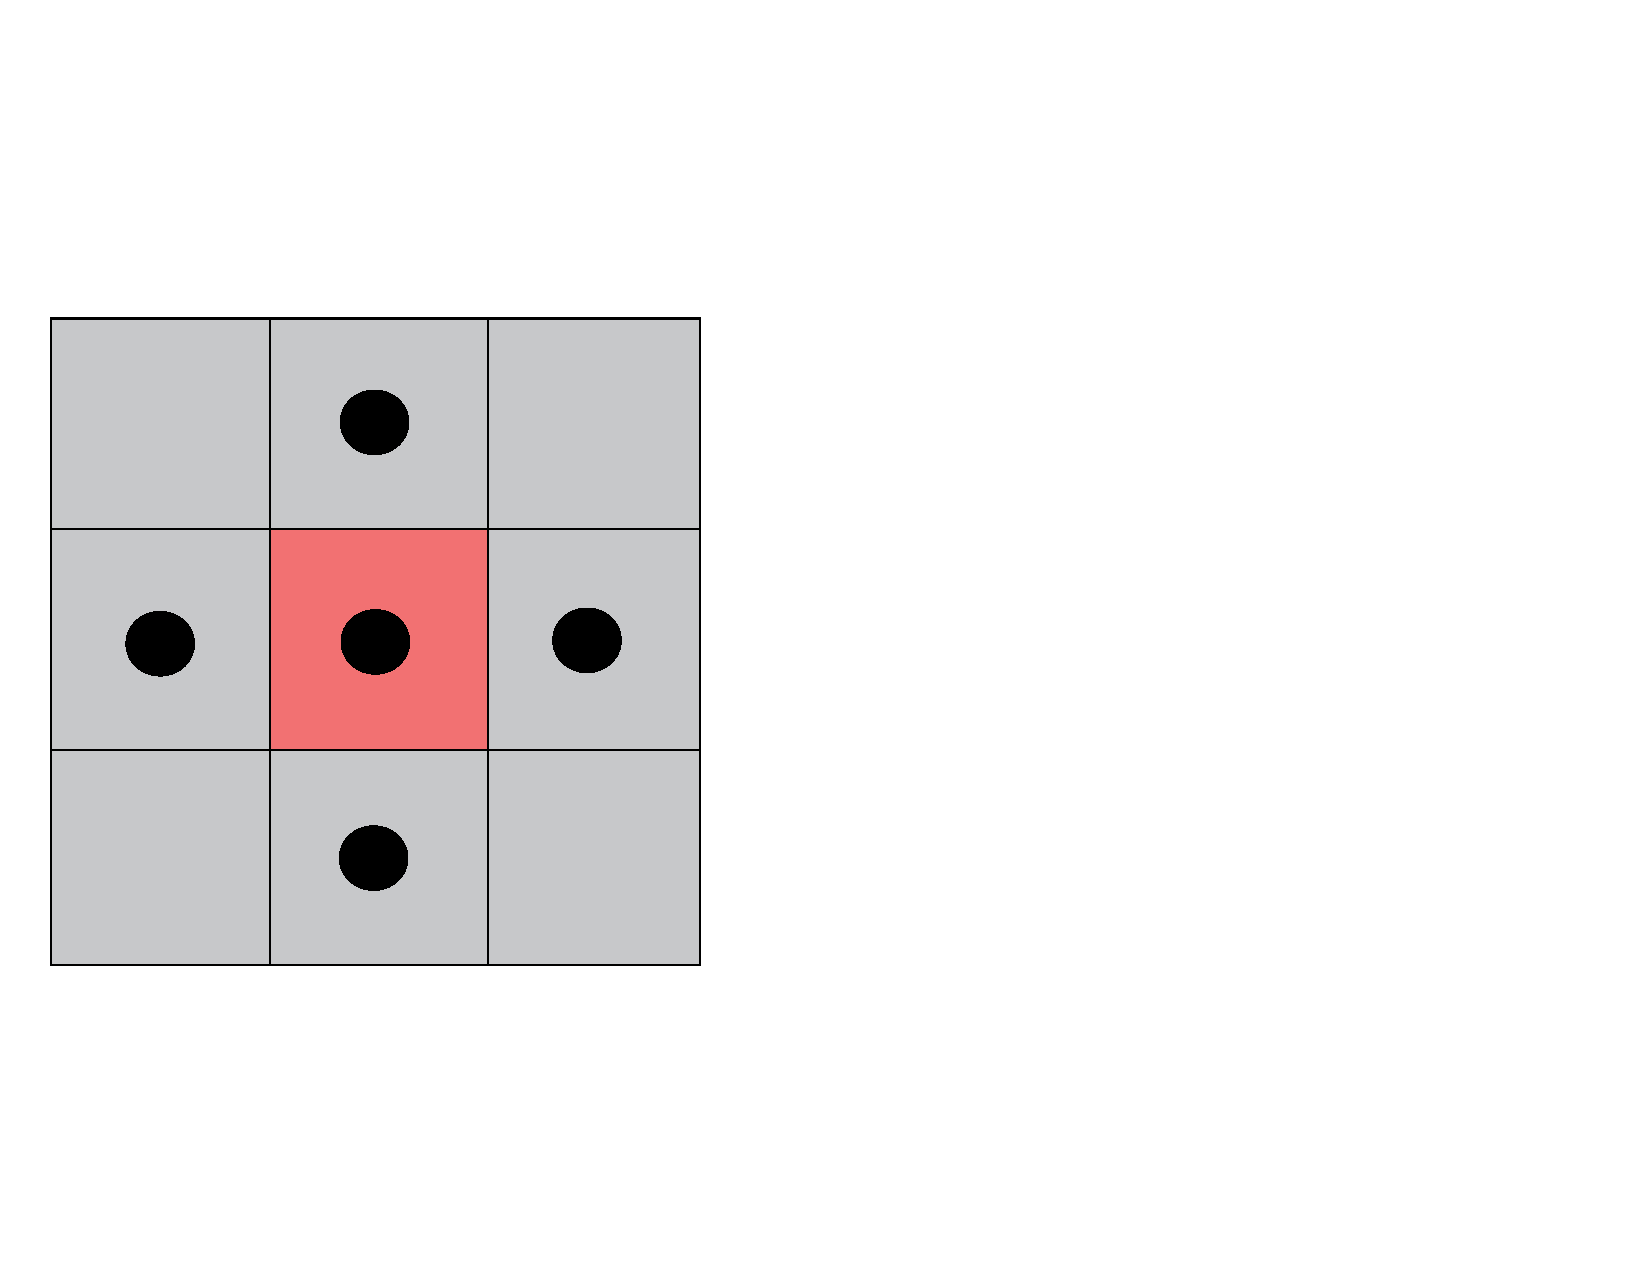
\includegraphics[width=0.6\linewidth]{figures/detection/4_pixel_connectivity.pdf}
    \caption{Four connectivity.}
    \label{fig:four_connectivity}
  \end{subfigure}
  \quad
  \begin{subfigure}[b]{0.3\textwidth}
    \centering
    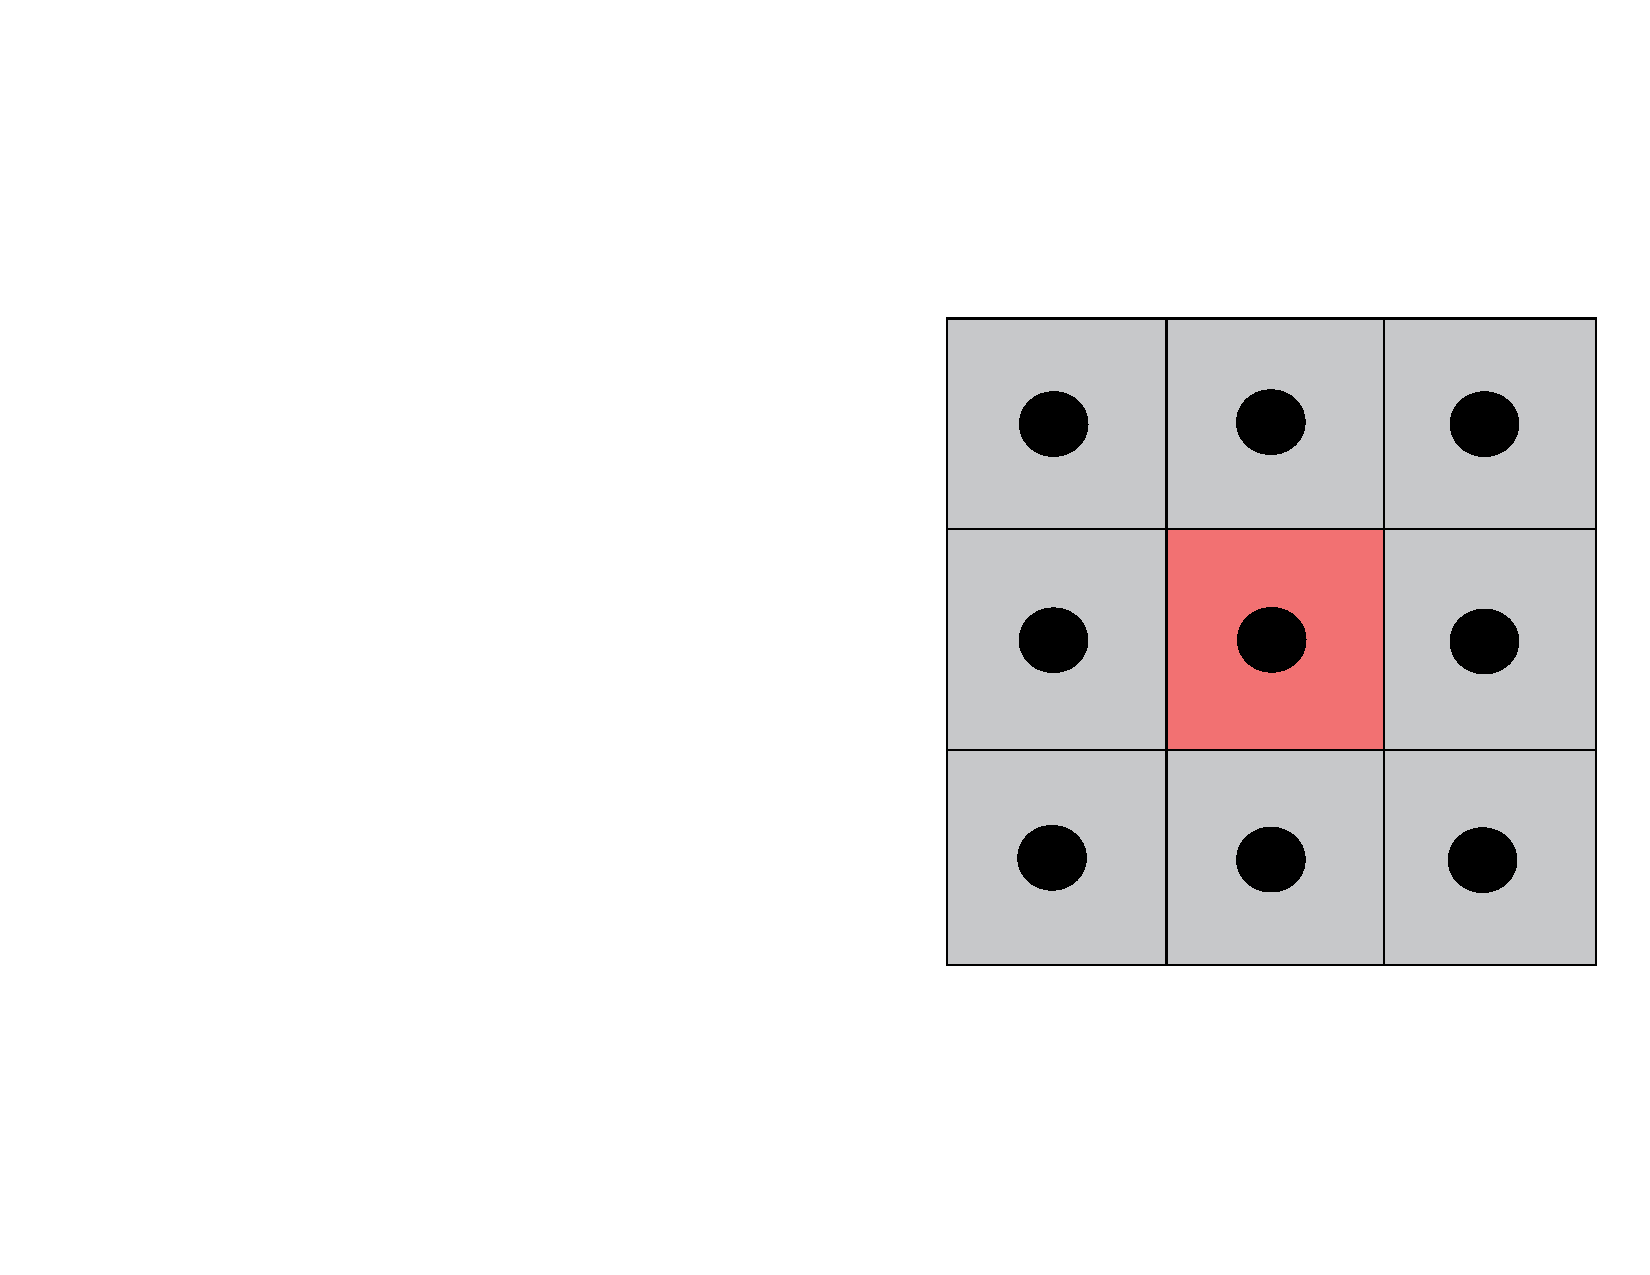
\includegraphics[width=0.6\linewidth]{figures/detection/8_pixel_connectivity.pdf}
    \caption{Eight connectivity.}
    \label{fig:eight_connectivity}
  \end{subfigure}
  \caption{Connected components labelling connectivity.}
  \label{fig:ccl_connectivity}
\end{figure}

Various algorithms exist to perform \gls{ccl}. Two of the most commonly used algorithms are the two-pass algorithm and the breadth-first single-pass algorithm. The two-pass algorithm is generally faster for images with large connected components and the breadth-first single-pass algorithm is generally faster for images with small connected components. The nature of the mosquito and laser detection is such that the connected components will be small, thus the breadth-first single-pass algorithm was chosen. The breadth-first single-pass algorithm is presented in \autoref{alg:single_pass_ccl}.
\begin{algorithm}[!htb]
  \caption{Breadth-First Single-Pass Connected Component Labelling}
  \label{alg:single_pass_ccl}
  \begin{algorithmic}[1]
    \Procedure{SinglePassCCL}{$image$}
    \State $rows, cols \gets \text{dimensions of } image$
    \State $label \gets 1$
    \State $labels \gets \text{2D array of zeros of size } rows \times cols$
    \For{$y \gets 0$ to $rows-1$}
    \For{$x \gets 0$ to $cols-1$}
    \If{$image[y][x] = 1$ and $labels[y][x] = 0$}
    \State $\text{ExploreBlob}(image, labels, x, y, label)$
    \State $label \gets label + 1$
    \EndIf
    \EndFor
    \EndFor
    \EndProcedure
    \State
    \Procedure{ExploreBlob}{$image, labels, x, y, label$}
    \State $queue \gets \text{empty queue}$
    \State $\text{Enqueue}(queue, (x, y))$
    \While{$\text{not empty}(queue)$}
    \State $(x, y) \gets \text{Dequeue}(queue)$
    \If{$x < 0$ or $x \geq cols$ or $y < 0$ or $y \geq rows$ or $image[y][x] = 0$ or $labels[y][x] > 0$}
    \State \text{continue}
    \EndIf
    \State $labels[y][x] \gets label$
    \For{each neighbour $(nx, ny)$ of $(x, y)$}
    \State $\text{Enqueue}(queue, (nx, ny))$
    \EndFor
    \EndWhile
    \EndProcedure
  \end{algorithmic}
\end{algorithm}



\subsubsection{Distinguishing between the laser's reflections}
The laser must shine through the front glass of the mosquito enclosure. This results in various reflections of the laser beam. There are three predominate reflections that can not be distinguished using a brightness threshold. These reflections are:
\begin{itemize}
  \item The reflection of the laser beam off the front glass at the origin of the laser turret, resulting from scattered light off the turret mirrors.
  \item The reflection of the laser beam incident on the front glass.
  \item The reflection of interest, which is the reflection of the laser beam incident on a mosquito or the back surface of the enclosure.
\end{itemize}

The reflection off the front glass at the origin of the laser turret remains stationary since the laser turret itself is stationary with only the angles of the mirrors changing. Thus, this reflection can be manually distinguished by drawing a bounding box around its position in the frame. The remaining two reflections are distinguished using the geometric properties of the system positioning. The $yz$-plane of the system is shown in \autoref{fig:distinguish_lasers} showing the potential laser beam paths for various turret angles. The laser turret is slightly below the camera which is exaggerated in \autoref{fig:distinguish_lasers} for illustration purposes. It can be seen in \autoref{fig:distinguish_lasers} that if both detections are at or below the camera origin, the reflection of interest is closer to the camera origin. If both reflections are at or above the camera origin, then the  reflection of interest is further from the camera origin. If the reflections are on either side of the camera origin, the reflection of interest is the reflection above the camera origin. This logic is easily extended to three dimensions by considering the $yz$-plane and $xz$-plane independently.
\begin{figure}[!htb]
  \centering
  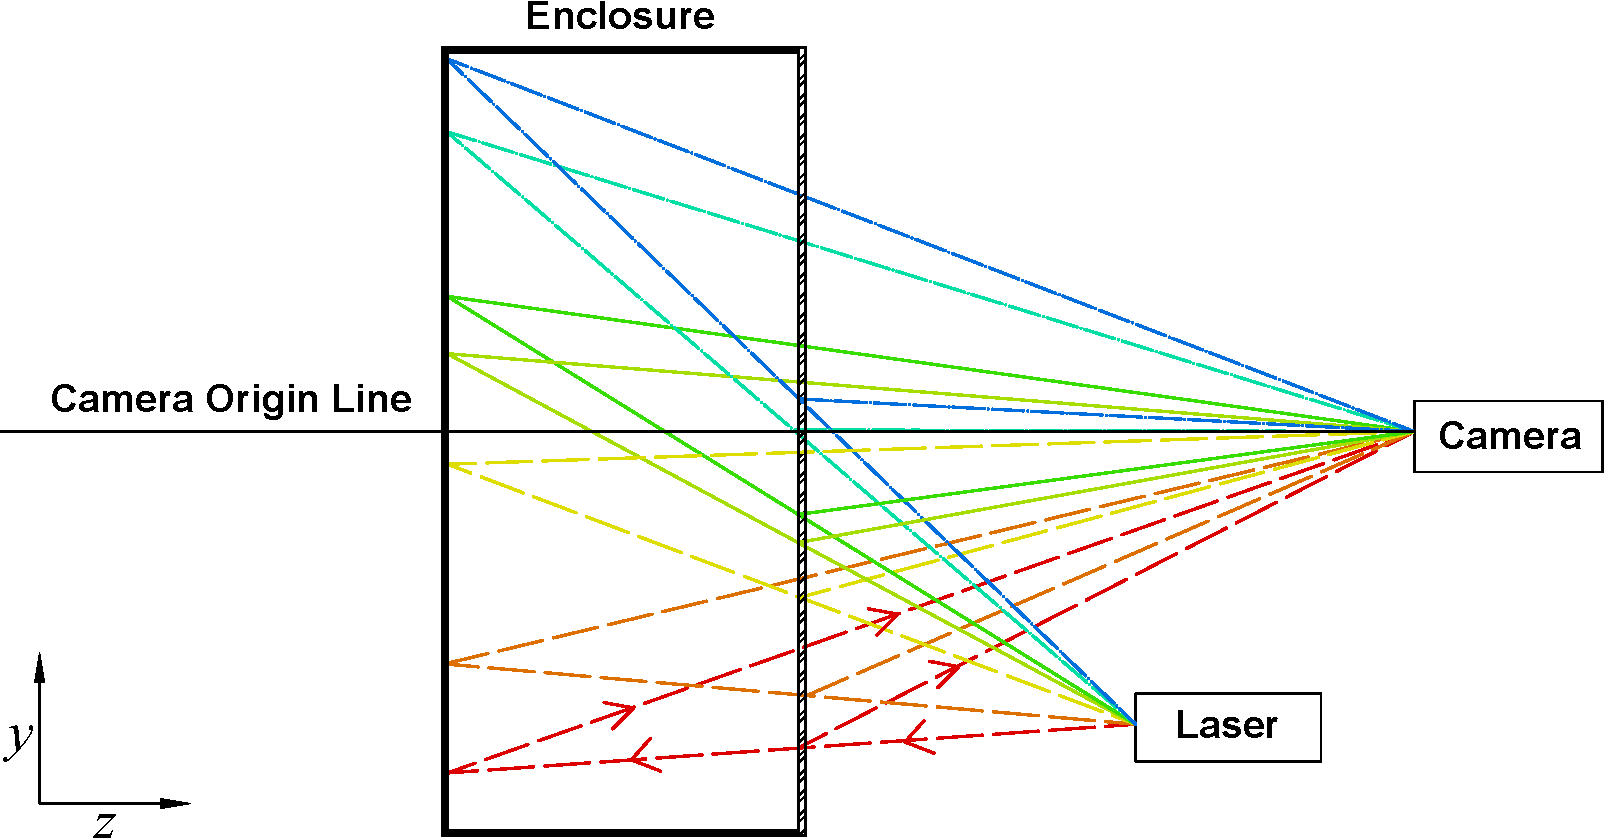
\includegraphics[width=\textwidth]{figures/distinguish_lasers.pdf}
  \caption{Distinguishing between the laser's reflections.}
  \label{fig:distinguish_lasers}
\end{figure}



\subsubsection{Mosquito tracking}\label{subsubsec:mosquito_tracking}
The mosquito tracking was performed using the \gls{sort} algorithm. The \gls{sort} algorithm is based on the tracking-by-detection paradigm, which means it relies on an external object detector. The object detector used was the mosquito detection algorithm described in \autoref{subsubsec:mosquito_and_laser_detection}. The \gls{sort} algorithm associates the detections across frames to create tracks.


\paragraph{Tracks}\mbox{}\\
The mosquito tracks are created using the Kalman filter. The theoretical background of Kalman filter is discussed in \autoref{subsubsec:kalman_filter}. The kinematic equation representing the flight of a mosquito must be defined to determine the state space of the Kalman filter. The kinematic equation used to model the flight of a mosquito is
\begin{equation}
  \label{eq:mosquito_kinematic_equation}
  \mathbf{x}_{k} = \mathbf{x}_{k-1} + \mathbf{\dot{x}}_{k-1}\Delta t + \frac{1}{2}\mathbf{\ddot{{x}}}_{k-1}\Delta t^2\,,
\end{equation}
where $\mathbf{x}_{k}$ is the position vector defined by the 2D pixel co-ordinate of a mosquito $[\:x\;\;\;y\:]^\mathrm{T}$. A constant velocity model with acceleration as noise will be used since mosquitoes have an erratic flight pattern. Therefore, the set of differential equations describing the state space of the Kalman filter is
\begin{equation}
  \begin{split}
    \mathbf{x}_k
    & = \mathbf{Ax}_{k-1} + \mathbf{Bu}_k + \mathbf{w}_k\,, \\
    \begin{bmatrix}
      x_k       \\
      y_k       \\
      \dot{x}_k \\
      \dot{y}_k
    \end{bmatrix}
    & =
    \begin{bmatrix}
      1 & 0 & \Delta t & 0        \\
      0 & 1 & 0        & \Delta t \\
      0 & 0 & 1        & 0        \\
      0 & 0 & 0        & 1
    \end{bmatrix}
    \begin{bmatrix}
      x_{k-1}       \\
      y_{k-1}       \\
      \dot{x}_{k-1} \\
      \dot{y}_{k-1}
    \end{bmatrix}\,,
  \end{split}
\end{equation}
where $\mathbf{u}_k$ is the input vector, which is the acceleration of the mosquito according to its kinematic flight model defined in \autoref{eq:mosquito_kinematic_equation}. However, this acceleration is unknown and will be compensated for by the process noise $\mathbf{w}_k$, thus $\mathbf{u}_k = \mathbf{0}$. The process noise $\mathbf{w}_k$ is assumed to be drawn from a zero mean multivariate normal distribution $\mathcal{N}$ with covariance $\mathbf{Q}_k$. Hence, $\mathbf{w}_k \sim$ $\mathcal{N}$ $\left(0, \mathbf{Q}_k\right)$. Thus, $\mathbb{E}[w_k] = 0$ and $\mathbb{E}[w_kw_k^\mathrm{T}] = \mathbf{Q}_k$. The process noise covariance matrix $\mathbf{Q}$ is given by
\begin{equation}
  \label{eq:kalman_filter_process_noise_covariance_matrix}
  \mathbf{Q} = \begin{bmatrix}
    \sigma_{x}^2               & 0                          & \sigma_{x}\sigma_{\dot{x}} & 0                          \\
    0                          & \sigma_{y}^2               & 0                          & \sigma_{y}\sigma_{\dot{y}} \\
    \sigma_{\dot{x}}\sigma_{x} & 0                          & \sigma_{\dot{x}}^2         & 0                          \\
    0                          & \sigma_{\dot{y}}\sigma_{y} & 0                          & \sigma_{\dot{y}}^2
  \end{bmatrix}\,,
\end{equation}
where $\sigma_{x}$ and $\sigma_{\dot{x}}$ are the standard deviations of the position and velocity, respectively. The standard deviation of the position is defined as the standard deviation of the acceleration $\sigma_{\ddot{x}}$ multiplied by $\frac{1}{2}\Delta t^2$, since this is the effect that the acceleration will have on the position as shown in \autoref{eq:mosquito_kinematic_equation}. Similarly, the standard deviation of the velocity is defined as $\Delta t \sigma_{\ddot{x}}$. Therefore, the process noise covariance can be written as
\begin{equation}
  \mathbf{Q} =
  \sigma_{\ddot{x}}^{2}
  \begin{bmatrix}
    \frac{\Delta t^4}{4} & 0                    & \frac{\Delta t^3}{2} & 0                    \\
    0                    & \frac{\Delta t^4}{4} & 0                    & \frac{\Delta t^3}{2} \\
    \frac{\Delta t^3}{2} & 0                    & \Delta t^2           & 0                    \\
    0                    & \frac{\Delta t^3}{2} & 0                    & \Delta t^2
  \end{bmatrix}\,.
\end{equation}

The position of a mosquito is the only component of the state that is measured by the detection system. Thus, the observation matrix $\mathbf{H}$ is
\begin{equation}
  \mathbf{H} = \begin{bmatrix}
    1 & 0 & 0 & 0 \\
    0 & 1 & 0 & 0
  \end{bmatrix}\,.
\end{equation}
The measurement noise covariance matrix $\mathbf{R}$ is
\begin{equation}
  \mathbf{R} = \begin{bmatrix}
    \sigma_{x}^2 & 0            \\
    0            & \sigma_{y}^2
  \end{bmatrix}\,,
\end{equation}
where $\sigma_{x}^2$ and $\sigma_{y}^2$ are the variances of the position detected. The initial state covariance matrix $\mathbf{P}$ is given by
\begin{equation}
  \mathbf{P} = \begin{bmatrix}
    \sigma_{x}^2 & 0            & 0               & 0               \\
    0            & \sigma_{y}^2 & 0               & 0               \\
    0            & 0            & \dot{x}_{max}^2 & 0               \\
    0            & 0            & 0               & \dot{y}_{max}^2
  \end{bmatrix}\,.
\end{equation}

The Kalman filter is initialised with the position of the mosquito as the initial state $\mathbf{x}_0$. The position of the mosquito in the next frame $\mathbf{\hat{x}}_{k\mid k-1}$ is predicted using the adapted predict equation of the Kalman filter $\mathbf{\hat{x}}_{k\mid k-1} = \mathbf{A}_k \mathbf{x}_{k-1\mid k-1}$. This prediction will be used in the association step before the update step. The update step of the Kalman filter is performed using the update equation of the Kalman filter $\mathbf{x}_{k\mid k} = \mathbf{x}_{k\mid k-1} + \mathbf{K}_k \left(\mathbf{z}_k - \mathbf{H}_k \mathbf{x}_{k\mid k-1}\right)$, where $\mathbf{K}_k$ is the Kalman gain and $\mathbf{z}_k$ is the measurement vector. The measurement vector $\mathbf{z}_k$ is the position of the mosquito detected in the current frame.


\paragraph{Association}\mbox{}\\
The association of tracks and detections will be done using the Hungarian algorithm, which is an optimised optimal assignment algorithm. The Hungarian algorithm has a time complexity of $O\left(n!\right)$ compared to the time complexity na\"ive approach $O\left(n^3\right)$. The Hungarian algorithm works as follows:
\begin{description}[style=nextline]
  \item[Generate a cost matrix.] Represent the problem with a square $n \times n$ matrix $\mathbf{C}$ where the element $\mathbf{C}_{i,j}$ represents the cost of assigning track $i$ to detection $j$. The cost function is the Euclidean distance between the predicted location and the detected location of the mosquito.
  \item[Row and column reduction.] Subtract the minimum value in each row from each element in the row. Perform the same operation for each column. This will produce a matrix with at least one zero in each row and column.
  \item[Cover zeros and check for optimality.] Cover all the zeros in the matrix using the minimum number of horizontal and vertical lines. If the minimum number of covering lines is $n$, an optimal assignment exists among the zeros, and the algorithm can proceed to the assignment phase. If not, you need to adjust the matrix and repeat from this step.
  \item[Adjust the matrix.] Find the smallest element that is not covered by any line. Subtract this element from all uncovered elements, and add it to all elements at the intersections of the covering lines. Return to \textit{cover zeros and check for optimality}.
  \item[Assignment.] Once an optimal assignment is found, read the assignment from the zeros in the matrix.
\end{description}



\subsubsection{Laser turret control system}
The laser turret control system is a closed-loop \gls{pid} controller. A \gls{pid} controller is represented by the following equation
\begin{equation}
  \label{eq:pid_controller}
  u(t) = K_p e(t) + K_i \int_{0}^{t} e(\tau) d\tau + K_d \frac{de(t)}{dt}\,,
\end{equation}
where $u(t)$ is the control signal, $e(t)$ is the error signal, $K_p$ is the proportional gain, $K_i$ is the integral gain, and $K_d$ is the derivative gain. The goal of the laser turret control system is to position the laser beam at the target co-ordinates. The target co-ordinates is defined by the mosquito detection and tracking system in pixels. The stepper motors are controlled in steps, thus the target pixels must be mapped to the number of steps required to move the laser beam to the target co-ordinates. The steps are defined in reference to the origin of the laser defined in \autoref{subsubsec:laser_turret_design}, which is the position when the laser beam is perpendicular to the $xy$-plane of the mosquito enclosure. The block diagram of the laser turret control system can be seen in \autoref{fig:control_system}. The two axes of the laser turret are controlled independently, each having their own \gls{pid} controller. The \gls{pid} controller is implemented in software and the control signal is sent to the stepper motor drivers using \gls{gpio}.
\begin{figure}[!htb]
  \centering
  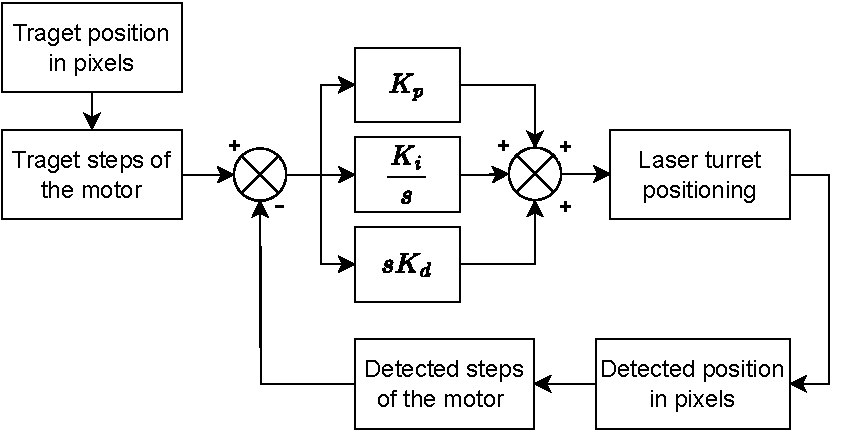
\includegraphics[width=0.8\textwidth]{figures/control_system.pdf}
  \caption{Laser turret control system.}
  \label{fig:control_system}
\end{figure}


\FloatBarrier
\subsection{Software implementation and optimisation}\label{subsec:software_implementation}
\subsubsection{Detection and tracking}
The resolution of the camera was set to $1280 \times 720$ and was cropped such that only the back wall of the mosquito enclosure is visible. This low resolution was selected to reduce the computational complexity of the image processing. The binarisation and image enhancement processes described in \autoref{subsubsec:mosquito_and_laser_detection} are suitable for parallelisation. Therefore, custom \gls{cuda} kernels were written to perform these operations on the Nvidia Jetson Nano \gls{gpu}. The kernel for the morphological erosion operation is shown in \autoref{lst:erosion_kernel} to demonstrate the structure of a \gls{cuda} kernel. Utilising the \gls{gpu} with kernels such as \autoref{lst:erosion_kernel} significantly improves the performance of the image processing system since the processing is performed concurrently across the 128 \gls{cuda} cores of the Nvidia Jetson Nano \gls{gpu}. The image processing is optimised using three \gls{cuda} kernels, one for binarisation, one for morphological erosion, and one for morphological dilation. These kernels are used 10 times per frame to perform the mosquito and laser detection. Thus, this optimisation has a significant impact on the performance of the system.

\begin{minipage}{\linewidth}
  \begin{lstlisting}[label={lst:erosion_kernel}, language=C++, caption={Erosion GPU kernel.}]
__global__ void erosion(uint8_t* input,
                        uint8_t* output,
                        uint8_t* struct_elem,
                        int struct_elem_radius) {
  int x = blockIdx.x * blockDim.x + threadIdx.x;
  int y = blockIdx.y * blockDim.y + threadIdx.y;
  
  if (x < d_COLS && y < d_ROWS) {
    int min_val = 255;
    for (int i = -struct_elem_radius; i <= struct_elem_radius; i++) {
      for (int j = -struct_elem_radius; j <= struct_elem_radius; j++) {
        if (y + i >= 0 && y + i < d_ROWS && x + j >= 0 && x + j < d_COLS) 
        {
          if (struct_elem[(i + struct_elem_radius) *
                          (2 * struct_elem_radius + 1) +
                          j + struct_elem_radius] == 1) 
          {
            int idx = (y + i) * d_COLS + (x + j);
            min_val = min(min_val, (int)input[idx]);
          }
        }
      }
    }
    output[y * d_COLS + x] = min_val;
  }
}
\end{lstlisting}
\end{minipage}


The Kalman filter was implemented as designed in \autoref{subsubsec:mosquito_tracking}. The matrix operations for the Kalman filter were implemented from first principles. Loops were used to perform the elementary operations on the individual elements of the matrices.

\subsubsection{Laser turret control}
The control of the laser turret required the following fundamental processes to be implemented:
\begin{itemize}
  \item Interfacing with stepper motor drivers.
  \item Converting pixels to steps.
\end{itemize}

% \paragraph{Interfacing with stepper motor drivers}\mbox{}\\
The stepper motors drivers were connected to the Nvidia Jetson Nano \gls{gpio} according to the diagram in \autoref{fig:stepper_driver_pins}.
\begin{figure}[!htb]
  \centering
  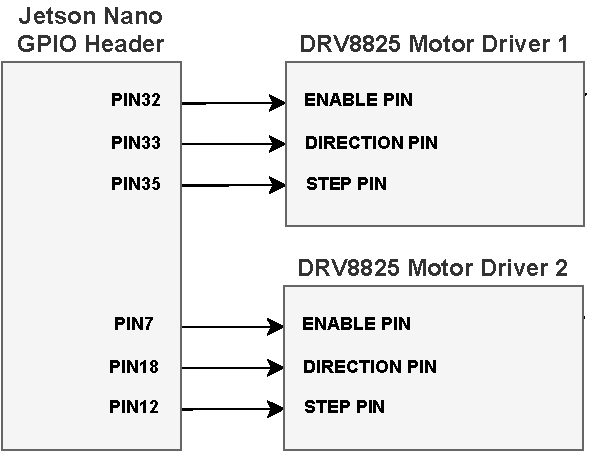
\includegraphics[width=0.6\textwidth]{figures/stepper_driver_pins.pdf}
  \caption{Stepper motor driver connections.}
  \label{fig:stepper_driver_pins}
\end{figure}
The motors are enabled by setting the "enable pin" to a logical high. The direction of rotation is determined by the logic level of the "direction pin". The stepper motors are driven by pulsing the "step pin" at the desired frequency for the required number of steps. This is shown in \autoref{alg:stepper_control}.
\begin{algorithm}[!htb]
  \caption{Stepper Motor Control}
  \label{alg:stepper_control}
  \begin{algorithmic}[1]
    \State $ENABLE\;PIN \gets \text{logical high}$
    \State $DIRECTION\;PIN \gets direction$
    \For{$step \gets 0$ to $steps-1$}
    \State $STEP\;PIN \gets \text{logical high}$
    \State $\text{delay}(period)$
    \State $STEP\;PIN \gets \text{logical low}$
    \State $\text{delay}(period)$
    \EndFor
  \end{algorithmic}
\end{algorithm}


% \paragraph{Converting pixels to steps}\mbox{}\\
The target position in pixels must be converted to the number of steps required to move the laser beam to the target position. This conversion is done using \autoref{eq:pixel_to_metric}, with the laser origin as the reference pixels. Hence, the motors steps are calculated in respect to the $45\degree$ origin position of the laser turret.

The major challenge in the implementation of the laser turret control system was the complete system integration required to achieve a functional discrete \gls{pid} controller.

\subsection{Final system integration}\label{subsec:integration}
The system was programmed in C++ and integrated into a single executable system. The system is required to operate in real-time. Therefore, the mosquito tracking and control of the laser turret must occur simultaneously. To achieve this, multi-threading was required. The multi-threaded implementation can be seen in the software flow diagram shown in \autoref{fig:software_flow_diagram}. Thread 1 performs the laser detection, mosquito detection, and mosquito tracking. Threads 2 and 3 are used to control each axis of the laser turret. The communication between threads is performed using atomic variables. This system enables the laser turret to continue adjusting the position of each axis to reach the target position while the video frames are processed to provide feedback for the laser turret control system and the updated position of the mosquito being targeted.
\begin{figure}[!htb]
  \centering
  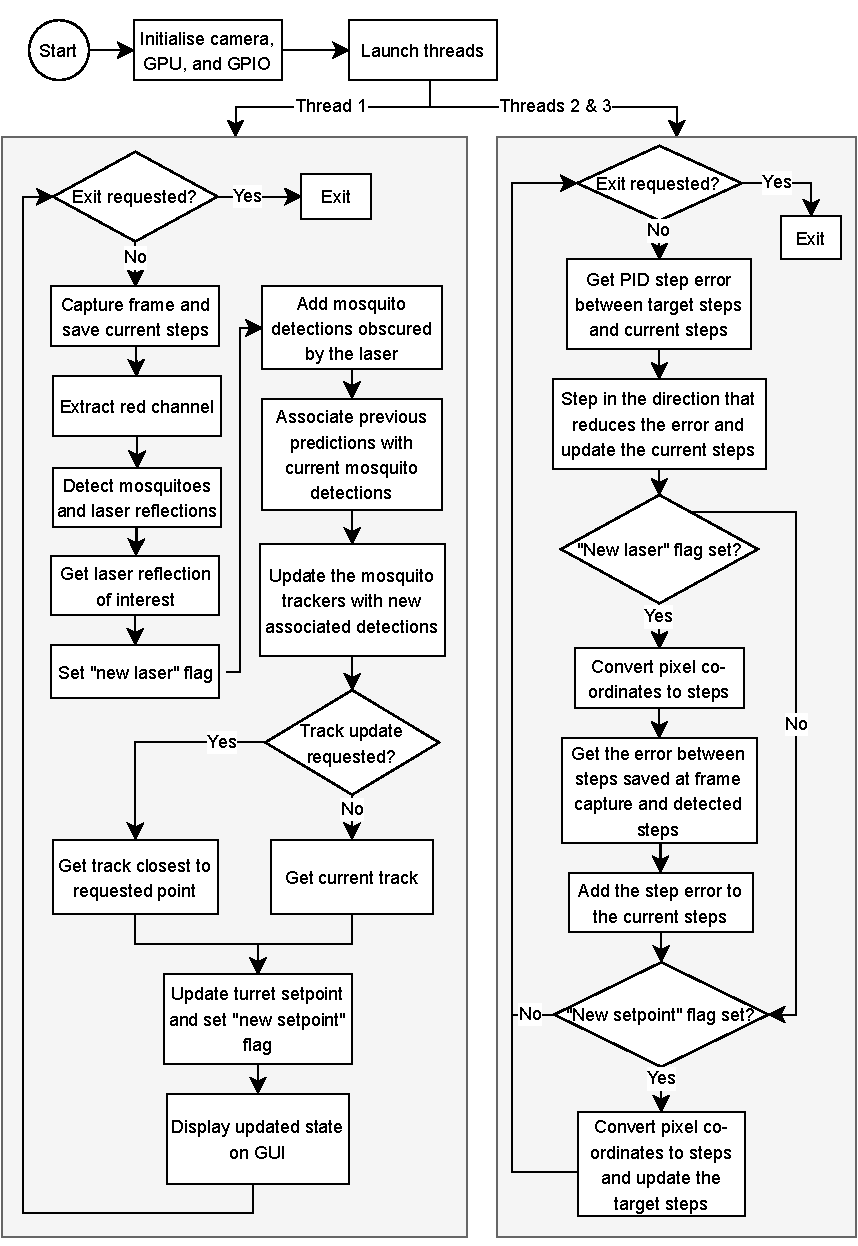
\includegraphics[width=0.95\textwidth]{figures/software_flow_diagram.pdf}
  \caption{Software flow diagram.}
  \label{fig:software_flow_diagram}
\end{figure}

The laser turret control system in threads 2 and 3 continuously poll flags that indicate whether there is new feedback available for laser position, and whether there is a new target position available. If either is available the control system breaks out of the loop that provides the pulses to drive the stepper motors. The new data is used to update required control action determined by the \gls{pid} controller. The system then resumes to drive the stepper motors until the control action is completed, or new data is available.

\newpage

%% End of File.


%%
%%  Department of Electrical, Electronic and Computer Engineering.
%%  EPR400/2 Final Report - Section 4.
%%  Copyright (C) 2011-2021 University of Pretoria.
%%

\section{Results}

\subsection{Summary of results achieved}
\begin{table}[H]
  \centering
  \begin{tabularx}{\textwidth}{|X|X|l|}
    \hline
    \textbf{Intended outcome}                                                                                                                                                    &
    \textbf{Actual outcome}                                                                                                                                                      &
    \textbf{Location in report}                                                                                                                                                                                                                                                                                                                                      \\
    \hline
    \multicolumn{3}{|l|}{\textbf{Core mission requirements and specifications}}                                                                                                                                                                                                                                                                                      \\
    \hline
    The system must track mosquitoes in a mosquito enclosure and illuminate a mosquito every 5 seconds.                                                                          &
    The system tracks mosquitoes in the enclosure and illuminates a mosquito under certain conditions                                                                            &
    Section 4.2.1                                                                                                                                                                                                                                                                                                                                                    \\
    \hline
    The laser must be able to illuminate a set point within 2 seconds accurate to within 1 millimetre.                                                                           &
    The laser is able to illuminate set point within 2 seconds accurate to within 1 millimetre.                                                                                  &
    Section 4.2.2                                                                                                                                                                                                                                                                                                                                                    \\
    \hline
    The system must be able to detect mosquitoes with a 90\% accuracy and 5\% false positive rate. The detection must be updated at least every 500 milliseconds.                & The system is able to detect mosquitoes with 90\% accuracy. The detection is updated every 500 milliseconds.                                            & Section 4.2.3           \\
    \hline
    The system must be able to track mosquitoes with 90\% accuracy of correct association between frames after 5 seconds.                                                        & The system is able to track mosquitoes with 90\% accuracy or correct association between frames.                                                        & Section 4.2.4           \\
    \hline
    \multicolumn{3}{|l|}{\textbf{Field condition requirements and specifications}}                                                                                                                                                                                                                                                                                   \\
    \hline
    Mosquitoes should be in an enclosure with controlled lighting and white lining on all the sides except the front facing side. The enclosure should be at least 1 metre wide. & The enclosure has \glspl{led} to control the lighting and white lining on all the sides except the front facing side. The enclosure is 0.9 metres wide. & Sections 4.2.1 to 4.2.4 \\
    \hline
    If mosquitoes cannot be obtained a suitable substitute will be used. The substitute will be a similar flying insect.                                                         & Mosquitoes and similar flying insects were obtained. Dead mosquitoes were also used.                                                                    & Sections 4.2.1 to 4.2.4 \\
    \hline
  \end{tabularx}
  \caption{Summary of results achieved.}
  \label{tab:results_summary}
\end{table}

\subsection{Qualification tests}
\textbf{Qualification test 1: Test of tracking and illuminating a mosquito}\\

\textit{Objectives of the test or experiment}\\
The objective of this experiment is to determine whether the system can track and illuminate a mosquito in the mosquito enclosure. The requirement states that the system must track mosquitoes in the enclosure and illuminate a mosquito every 5 seconds.

\textit{Equipment used}\\
The Nvidia Jetson Nano was used as the embedded platform to control the system. The Raspberry Pi Camera Module V2 was used to capture the video feed. The laser turret developed for this project was used to position the laser. The mosquito enclosure, laser turret, and camera was positioned as described in \autoref{subsubsec:system_positioning}. The Nvidia Jetson Nano was connected to user peripherals for user input and output. C++ code was developed specifically to capture the results for qualification test 1.

\textit{Test setup and experimental parameters}\\
Mosquitoes were simulated with a small black dot attached to a white shafts. The shafts were inserted into the enclosure and moved by hand to mimic the motion of mosquitoes.

\textit{Results or measurements}\\
The results from three different scenarios are presented in \Cref{fig:q1_1mos_detection_10fps,fig:q1_1mos_prediction_10fps,fig:q1_2mos_prediction_10fps}. The first scenario is where the laser is set to target the detected location of the mosquito. The second scenario is where the laser is set to target the predicted location of the mosquito. In the third scenario two mosquitoes were inserted into the enclosure and the laser was set to target the predicted locations of the mosquitoes.

\begin{figure}[h]
  \centering
  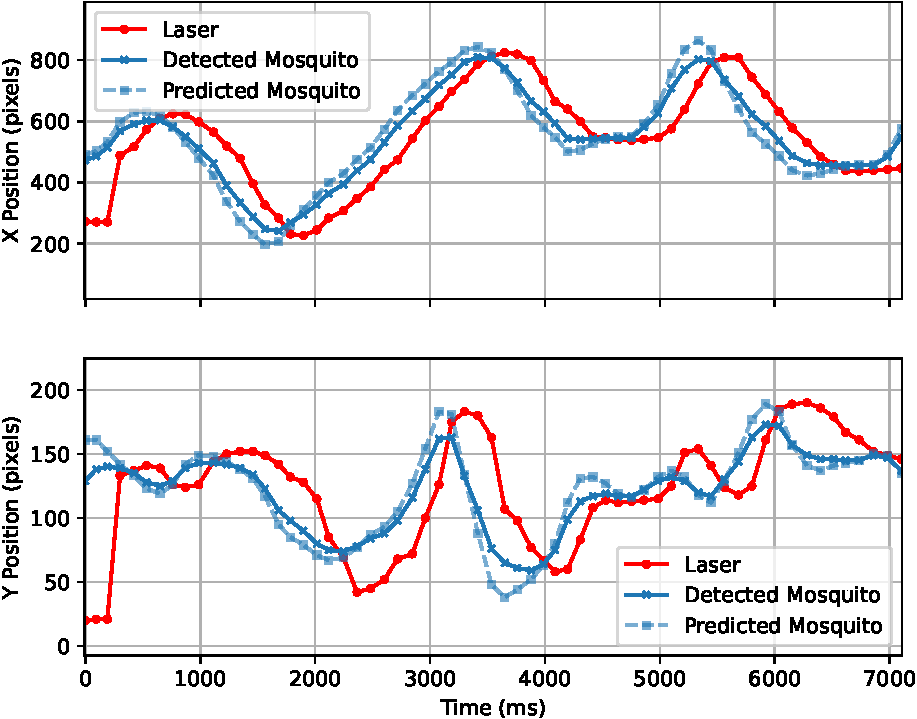
\includegraphics[width=0.8\textwidth]{figures/results/q1_1mos_detection_10fps.pdf}
  \caption{The position of the laser, detected mosquito, and predicted mosquito over time. The laser was set to target the detected location of the mosquito in this test.}
  \label{fig:q1_1mos_detection_10fps}
\end{figure}

\begin{figure}[h]
  \centering
  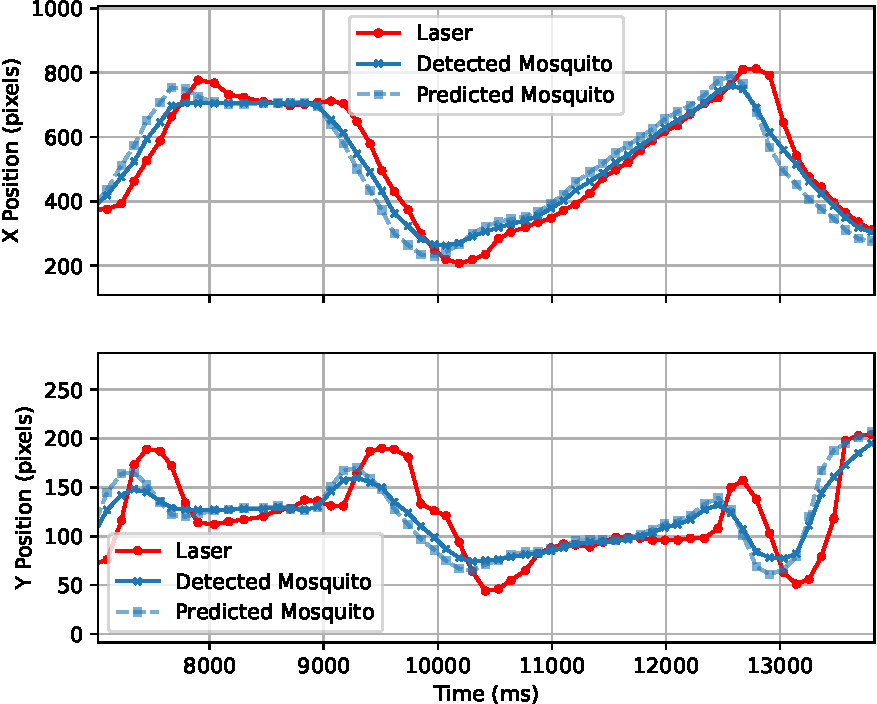
\includegraphics[width=0.8\textwidth]{figures/results/q1_1mos_prediction_10fps.pdf}
  \caption{The position of the laser, detected mosquito, and predicted mosquito over time. The laser was set to target the predicted location of the mosquito in this test.}
  \label{fig:q1_1mos_prediction_10fps}
\end{figure}

\begin{figure}[h]
  \centering
  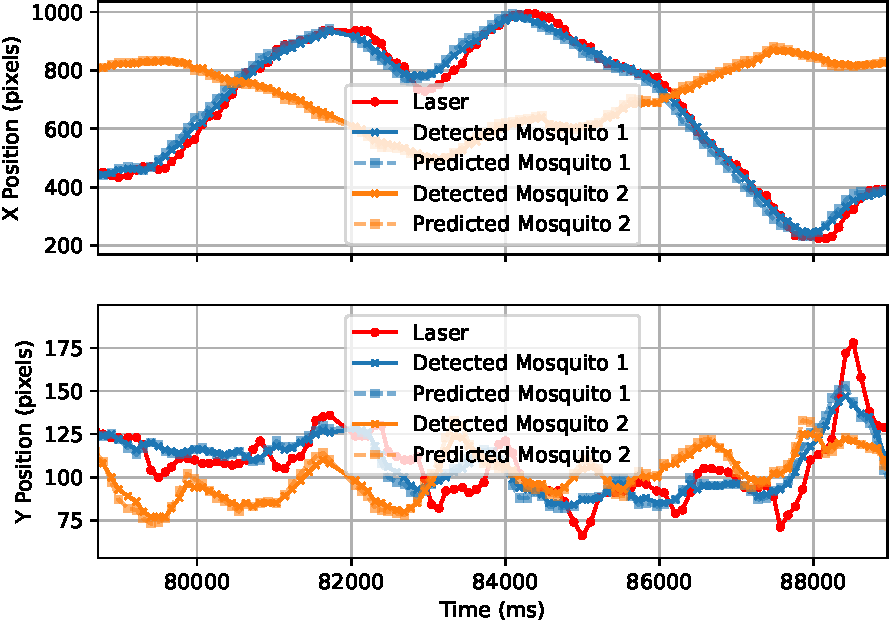
\includegraphics[width=0.95\textwidth]{figures/results/q1_2mos_prediction_10fps.pdf}
  \caption{The position of the laser, detected mosquitoes, and predicted mosquitoes with two mosquitoes in the enclosure over time. The laser was set to target the predicted location of the mosquito in this test.}
  \label{fig:q1_2mos_prediction_10fps}
\end{figure}

\textit{Observations}\\
In \Cref{fig:q1_1mos_detection_10fps,fig:q1_1mos_prediction_10fps,fig:q1_2mos_prediction_10fps}, it can be seen that the system is actively adjusting the position of the laser to track the mosquitos. In \autoref{fig:q1_1mos_detection_10fps}, the system was set to target the detected position of the mosquito. With this targeting technique it can be seen that the laser is trailing behind the actual position of the mosquito unless the mosquito is stationary. In \autoref{fig:q1_1mos_prediction_10fps}, the system was set to target the predicted position of the mosquito. With this targeting technique it can be seen that the laser reaches the actual position of the mosquito if the mosquito moves linearly for a sufficient amount of time. However, this targeting technique also results in significant overshoot when the mosquito changes direction. \autoref{fig:q1_2mos_prediction_10fps} shows the system tracking two mosquitoes in the enclosure. It can be seen that the system is able to track both mosquitoes simultaneously. The system selects one of the mosquitoes to target with the laser and the other mosquito is ignored by the laser. The same tracking behaviour is observed as in \autoref{fig:q1_1mos_prediction_10fps}, where the laser is set to target the predicted location of the mosquito.

\FloatBarrier
\textbf{Qualification test 2: Measurement of the time taken for the laser to reach a set point}\\

\textit{Objectives of the test or experiment}\\
The objective of this experiment is to measure the time it takes for the laser to reach a set point. The requirement states that the laser must be able to illuminate a set point within 2 seconds accurate to within 1 millimetre.

\textit{Equipment used}\\
The Nvidia Jetson Nano was used as the embedded platform to control the system. The Raspberry Pi Camera Module V2 was used to capture the video feed. The laser turret developed for this project was used to position the laser. The mosquito enclosure, laser turret, and camera was positioned as described in \autoref{subsubsec:system_positioning}. The Nvidia Jetson Nano was connected to user peripherals for user input and output. C++ code was developed specifically to capture the results for qualification test 2.

\textit{Test setup and experimental parameters}
\begin{enumerate}
  \item The set point was set to an arbitrary location in the mosquito enclosure.
  \item The laser was manually positioned to an arbitrary location in the mosquito enclosure.
  \item The laser turret control system was activated.
  \item The time and position of the laser was recorded for each frame captured by the system until the laser reached a settling point.
  \item Steps 1 to 4 were repeated.
\end{enumerate}

\textit{Results or measurements}\\
\autoref{fig:q2_laser_to_setpoint} shows the position of the laser over time for multiple runs with different starting points with a constant set point. \autoref{fig:q2_laser_errors} shows the euclidean distance between the laser and the set point in pixels for multiple runs with different starting points and set points. \autoref{fig:q2_laser_errors} has been restricted to the time range of 1200 to 2200 milliseconds such that the exact error between laser and set point can be observed. The radius of the laser was measured to a minimum of 5 pixels. The radius of a 2 millimetre disc was measured to be an average 2 pixels.

\begin{figure}[h]
  \centering
  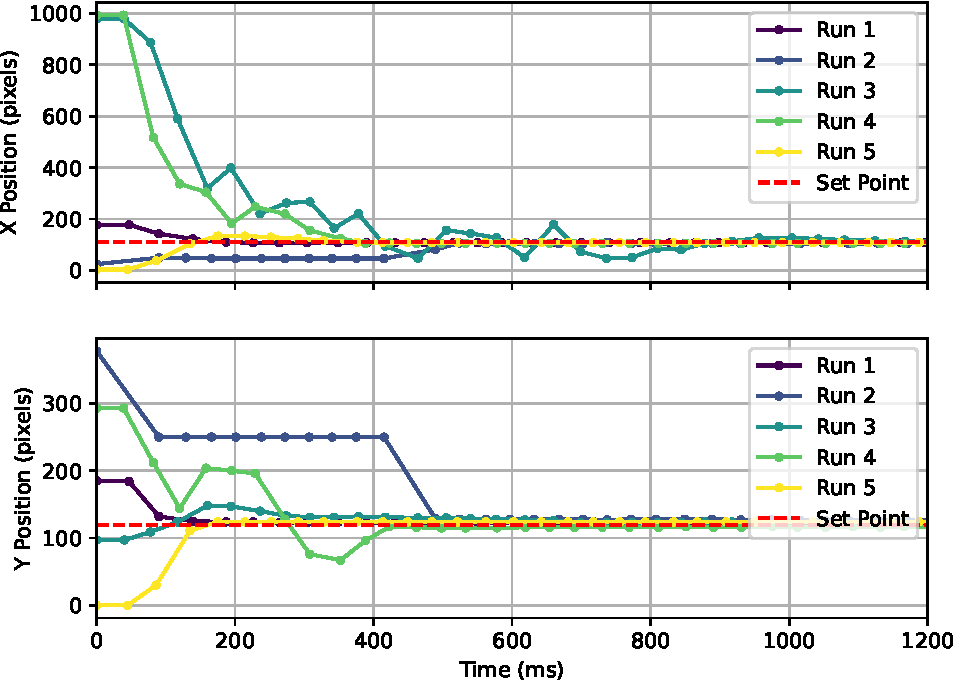
\includegraphics[width=\textwidth]{figures/results/q2.pdf}
  \caption{The position of the laser over time for multiple runs with different starting points with a constant set point.}
  \label{fig:q2_laser_to_setpoint}
\end{figure}

\begin{figure}[h]
  \centering
  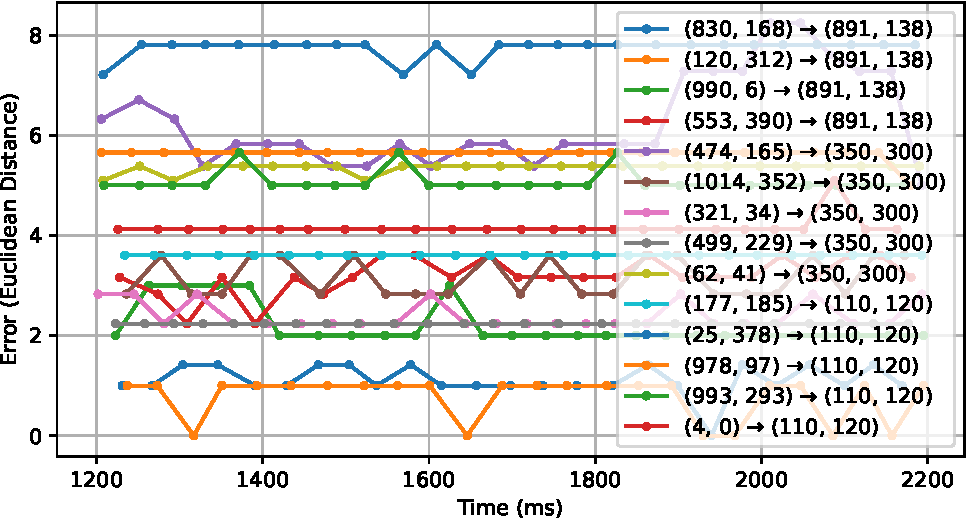
\includegraphics[width=\textwidth]{figures/results/q2_errors.pdf}
  \caption{The euclidean distance between the laser and the set point in pixels for multiple runs with different starting points and set points.}
  \label{fig:q2_laser_errors}
\end{figure}

\textit{Observations}\\
\autoref{fig:q2_laser_to_setpoint} shows the position of the laser over time for multiple runs with different starting points with a constant set point. It can be seen that general behaviour of the control system adjusts the position of the laser to move towards the set point. \autoref{fig:q2_laser_errors} shows the euclidean distance between the laser and the set point in pixels for multiple runs with different starting points and set points. The graph is restricted to the time range of 1200 to 2200 milliseconds which is after the position of the laser has stabilised. It can be seen from the various tests that the maximum euclidean distance between the laser and the set point is less the 8 pixels.

\FloatBarrier
\textbf{Qualification test 3: Test of mosquito detection}\\

\textit{Objectives of the test or experiment}\\
The objective of this experiment is to determine whether the system can detect mosquitoes in the mosquito enclosure. The requirement states that the system must be able to detect mosquitoes with a 90\% accuracy and 5\% false positive rate. The detection must be updated at least every 500 milliseconds.

\textit{Equipment used}\\
The Nvidia Jetson Nano was used as the embedded platform to control the system. The Raspberry Pi Camera Module V2 was used to capture the video feed. The laser turret developed for this project was used to position the laser. The mosquito enclosure, laser turret, and camera was positioned as described in \autoref{subsubsec:system_positioning}. The Nvidia Jetson Nano was connected to user peripherals for user input and output. C++ code was developed specifically to capture the results for qualification test 3.

\textit{Test setup and experimental parameters}\\
Mosquitoes and similar flying insect specimens were glued to white shafts as shown in \autoref{fig:dead_mossies}.
\begin{figure}
  \centering
  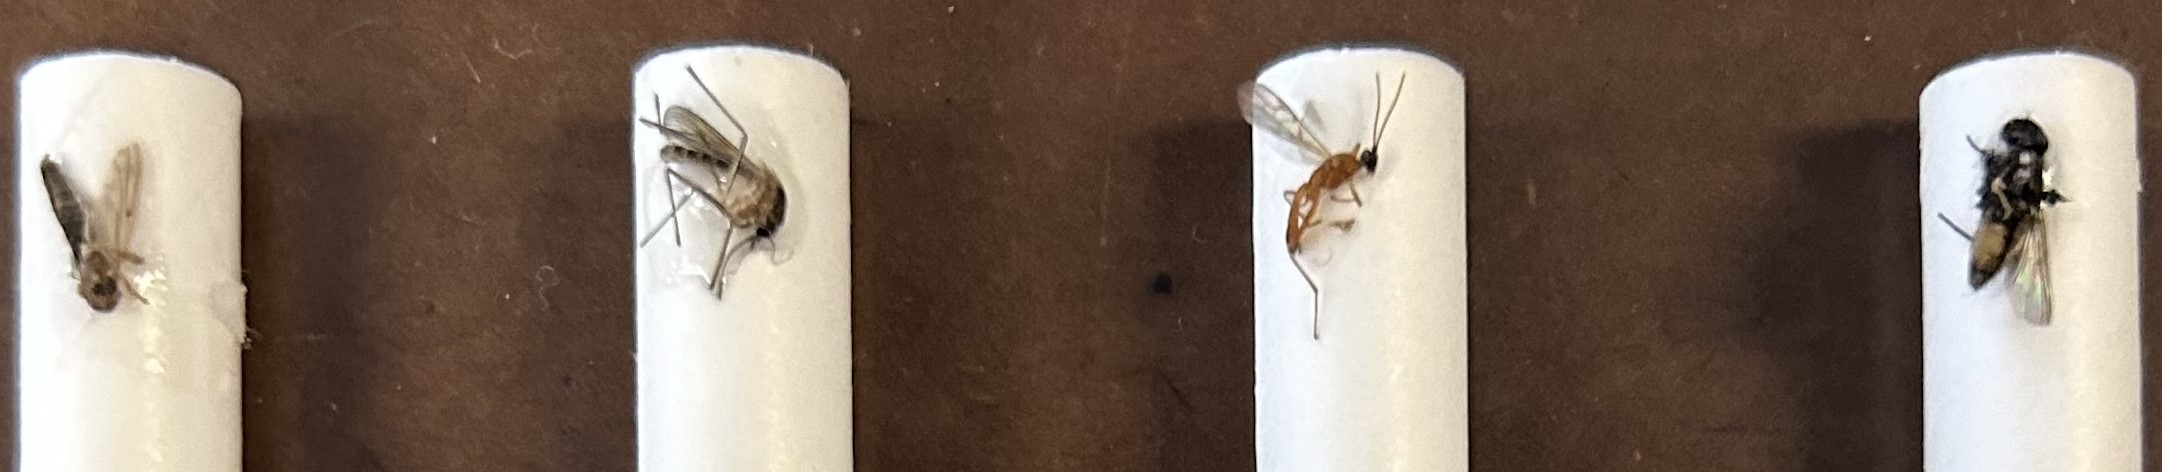
\includegraphics[width=0.8\textwidth]{figures/results/dead_mossies.jpg}
  \caption{Dead mosquitoes glued to white shafts.}
  \label{fig:dead_mossies}
\end{figure}

The test procedure was as follows:
\begin{enumerate}
  \item A known number of mosquitoes were inserted into the enclosure.
  \item The detection system was activated for 100 frames.
  \item The number of mosquitoes detected in each frame was recorded as well as the time between each frame.
  \item The experiment was repeated for different amounts of mosquitoes in the enclosure.
\end{enumerate}

\textit{Results or measurements}\\
The detection accuracy and false positive rate was determined using
\begin{equation}
  \text{Accuracy} = \frac{\text{TP} + \text{TN}}{\text{TP} + \text{TN} + \text{FP} + \text{FN}}\,,
\end{equation}
and
\begin{equation}
  \text{False positive rate (FPR)} = \frac{\text{FP}}{\text{FP} + \text{TN}}\,,
\end{equation}

where TP is the number of true positives, TN is the number of true negatives, FP is the number of false positives, and FN is the number of false negatives. The detection time requirement was determined by calculating the time between each frame.

Four tests were conducted using the test procedure described above. The results were captured for 0, 1, 2, and 3 mosquitoes in the enclosure. The true positives, false positives, false negatives, and true negatives for the combined tests are shown in \autoref{fig:detection}. The detection update interval is shown in \autoref{fig:detection_frequency}.
\begin{figure}[h]
  \centering
  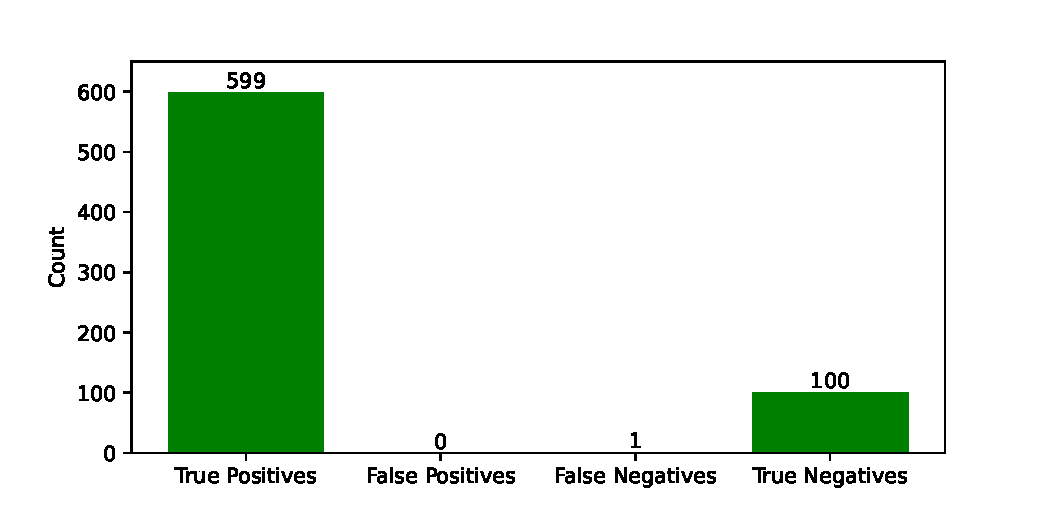
\includegraphics[width=\textwidth]{figures/results/detection.pdf}
  \caption{Mosquito detections.}
  \label{fig:detection}
\end{figure}
\begin{figure}[h]
  \centering
  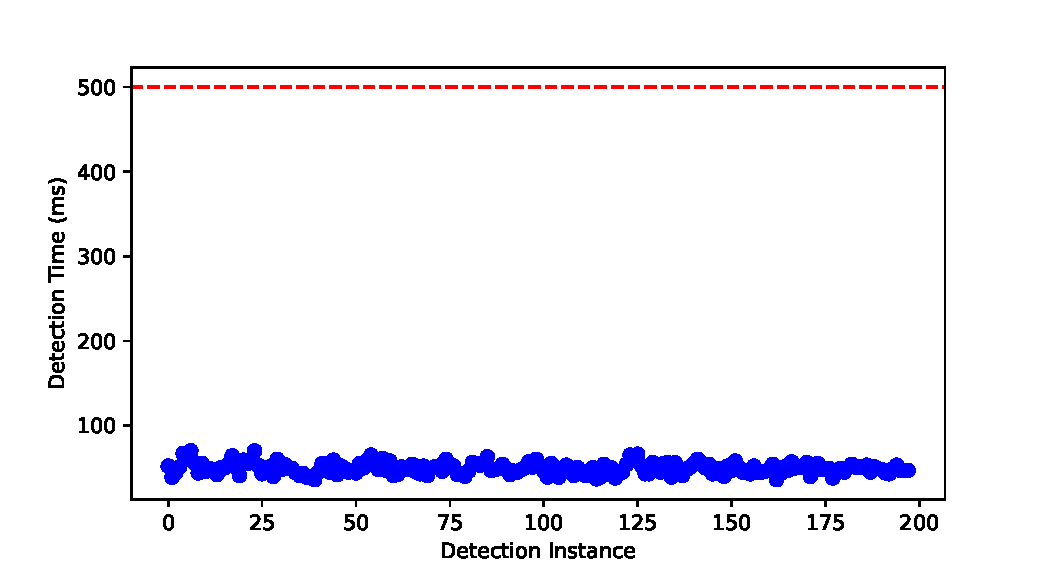
\includegraphics[width=\textwidth]{figures/results/detection_frequency.pdf}
  \caption{Mosquito detection update interval.}
  \label{fig:detection_frequency}
\end{figure}
The detection results for qualification test 3 are summarised in \autoref{tab:detection_results}
\begin{table}[h]
  \centering
  \begin{tabular}{|l|l|}
    \hline
    \textbf{Metric}     & \textbf{Value} \\
    \hline
    True Positives      & 599            \\
    False Positives     & 0              \\
    False Negatives     & 1              \\
    True Negatives      & 100            \\
    Accuracy            & 0.998571       \\
    False Positive Rate & 0.0            \\
    \hline
  \end{tabular}
  \caption{A summary of the detection results.}
  \label{tab:detection_results}
\end{table}

\textit{Observations}\\
The system performs detections within 100 milliseconds which is well within the 500 millisecond requirement. The system is able to detect mosquitoes with a 99\% accuracy and 0\% false positive rate.

\FloatBarrier
\textbf{Qualification test 4: Test of mosquito tracking}\label[section]{sec:tracking_quali}\\
\textit{Objectives of the test or experiment}\\
The objective of this experiment is to determine whether the system can track mosquitoes in the mosquito enclosure. The requirement states that the system must track mosquitoes in the enclosure with 90\% correct association after 5 seconds.

\textit{Equipment used}\\
The Nvidia Jetson Nano was used as the embedded platform to control the system. The Raspberry Pi Camera Module V2 was used to capture the video feed. The laser turret developed for this project was used to position the laser. The mosquito enclosure, laser turret, and camera was positioned as described in \autoref{subsubsec:system_positioning}. The Nvidia Jetson Nano was connected to user peripherals for user input and output. C++ code was developed specifically to capture the results for qualification test 4.

\textit{Test setup and experimental parameters}\\
Mosquitoes were simulated with a small black dot attached to a white shafts.

\begin{enumerate}
  \item The mosquito shafts were inserted into the enclosure.
  \item The data capturing procedure was started.
  \item The mosquito moved by hand to mimic the motion of mosquitoes.
  \item The data capturing procedure automatically stops after 100 frames have been recorded.
\end{enumerate}

\textit{Results or measurements}\\
\autoref{fig:q4_tracking} shows the detected and predicted position of the tracked mosquitoes in the camera pixel co-ordinate system.
\begin{figure}[h]
  \centering
  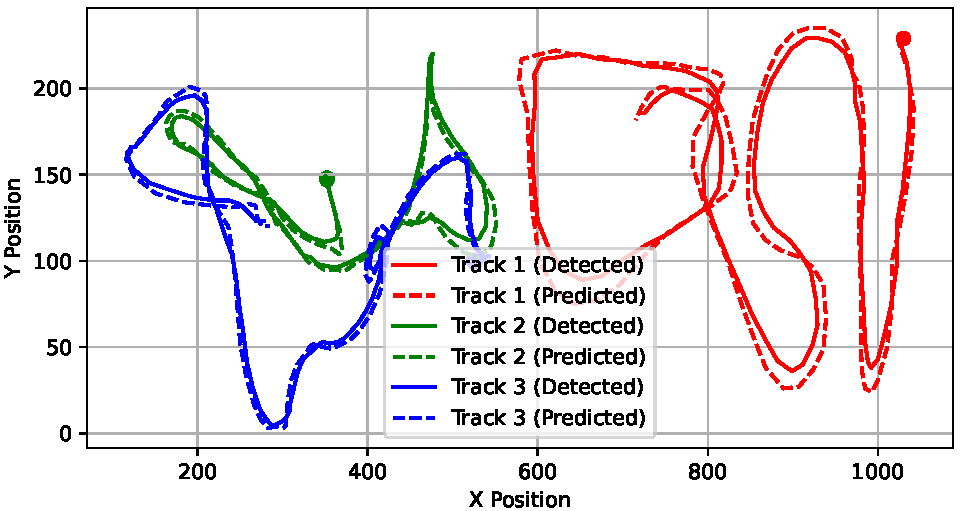
\includegraphics[width=\textwidth]{figures/results/tracking.pdf}
  \caption{The detected and predicted position of the tracked mosquitoes in the camera pixel co-ordinate system.}
  \label{fig:q4_tracking}
\end{figure}

\textit{Observations}\\
In \autoref{fig:q4_tracking}, it can be seen that the system is able correctly associate the mosquitoes between frames. The detected and predicted paths travelled by the mosquitoes are plotted. It can be seen that the predicted locations significantly deviates from the detected locations when there is a change in the direction of the path travelled by the mosquito. Three mosquitoes were tracked in this test.

\newpage

%% End of File.



%%
%%  Department of Electrical, Electronic and Computer Engineering.
%%  EPR400/2 Final Report - Section 5.
%%  Copyright (C) 2011-2021 University of Pretoria.
%%

\section{Discussion}

\subsection{Critical evaluation of the design}

\subsubsection{Interpretation of results}
\paragraph{Laser turret}\hfill\\
It can be seen in \autoref{fig:q2_laser_to_setpoint} that laser turret responds rapidly to a step input. The laser turret reaches a settling point within 600\,ms of the step input for all runs in \autoref{fig:q2_laser_to_setpoint} other than run 3, which reached a settling point within 1200\,ms. The system specification requires the laser turret to reach a settling point within 2 seconds. The response time of the laser turret is well within this specification.

In \autoref{fig:q2_laser_errors}, it can be seen that the laser turret reaches the setpoint accurate to within 6 pixels for all tests with one exception. The system specification requires the laser turret to reach the setpoint accurate to within 1 millimetre. To determine whether this accuracy has been met the following measurements were made: the radius of the laser beam was measured to be a minimum of 5 pixels and the radius of a known 2-millimetre disc was measured to be an average 2 pixels. These two measurements indicate that the laser can be a maximum of 6 pixels away from the setpoint and still be within 1 millimetre of the setpoint. This indicates that all the test runs in \autoref{fig:q2_laser_errors}, except for one which has an error of 8 pixels, reach the setpoint accurate to within 1 millimetre. However, the radius of the laser beam and the know 2-millimetre disc do vary. The laser beam radius varies with the specific lighting conditions and the incident angle with the mosquito enclosure. The radii of the laser beam and disc also vary depending on the location in the camera frame in terms of the depth which they are from the camera and the lateral position in the camera frame since the camera is subject to lens distortion. This means that pixel distance that equates to 1 millimetre accuracy is not constant. The measurements of laser beam and disc radii were made conservatively such that the accuracy of the laser turret is likely to be better than 1 millimetre if it is within 6 pixels of the setpoint.

In run 1 of \autoref{fig:q2_laser_to_setpoint}, it can be seen that the laser plateaus for about 300\,ms before reaching the target position. This is likely due to a false negative laser detection. The laser position error is not updated for the period of false negative detections and thus no control action is taken since the control system is unaware of the error.


\paragraph{Mosquito detection}\hfill\\
From the bar graph in \autoref{fig:detection} it can be seen that the detection system produced 599 true positives, 0 false positives, 100 true negatives, and 1 false negative for the tests conducted. The system specification requires the detection system to have an accuracy of 90\% and a false positive rate of less than 5\%. The detection results indicate that the detection system has a 99\% accuracy and 0\% false positive rate. This is well within the system specification. However, the detection system was tested using a small set of specimens that were available. The specimens were dead mosquitoes and other similar flying insects that were glued to white shafts. The white shafts were moved by hand to mimic live mosquitoes. This test setup does not accurately represent the true appearance of live mosquitoes. The white shafts form shadows and other artefacts that are not present when detecting live mosquitoes. This reduces the range of pixel intensity values that can be considered for a potential mosquito detection. Therefore, the detection system could perform better with the given test specimens if it was not necessary to attach them to the white shafts.

\paragraph{Mosquito tracking}\hfill\\
In \autoref{fig:q4_tracking}, it can be seen that system is able to track multiple mosquitoes simultaneously. The tracking specification requires that mosquitoes are correctly associated between frames with 90\% accuracy. It can be seen by inspecting the systems tracked paths of the mosquitoes in \autoref{fig:q4_tracking} that the system has correctly associated the mosquitoes between frames with 100\% accuracy. This was determined by analysing the different flight paths captured. It can be seen that there is no other logical association of the flight paths other than the one shown in \autoref{fig:q4_tracking}. This system is able to correctly associate mosquitoes between frames with flight paths that cross each other. These results indicate that the tracking system meets the system specification. However, the tracking results were obtained using a small set of specimens that were moved by hand to mimic the true flight of mosquitoes. This does not accurately represent the true flight and behaviour of mosquitoes. The true flight of mosquitoes is likely to be more erratic than the mimicked flight. Real mosquitoes are also capable of crossing paths with trajectories that can lead to ambiguous identities that can result in incorrect association. However, for the performance of the overall system this should not be a concern since the ultimate goal of the system would be to kill all mosquitoes in the enclosure.

The tracking system does predict the future position of the mosquitoes, however it can be seen in \autoref{fig:q4_tracking} that when movement of the mosquitoes are highly non-linear this prediction is not accurate. This is because the system does not accurately model the movement of the mosquitoes. The acceleration of the mosquitoes are modelled are system noise since the acceleration of the mosquitoes cannot be accurately model due to their erratic movement.

\paragraph{Overall system performance}\hfill\\
The graphs in \Cref{fig:q1_1mos_detection_10fps,fig:q1_1mos_prediction_10fps,fig:q1_2mos_prediction_10fps} illustrate the performance of the system as a whole. \autoref{fig:q1_2mos_prediction_10fps} demonstrates the system's ability to track multiple mosquitoes simultaneously while targeting the mosquitoes with the laser. When multiple mosquitoes are tracked the system only targets the selected mosquito with the laser and ignores the other mosquitoes. The system can be seen to correctly target a single mosquito in the presence of other mosquitoes in \autoref{fig:q1_2mos_prediction_10fps}. The accuracy of the targeting system can be seen in \autoref{fig:q1_1mos_prediction_10fps}. In \autoref{fig:q1_1mos_prediction_10fps}, it can be seen that the laser is able to consistently remain near the position of the mosquito regardless of the movement of the mosquito. However, the laser is only able to illuminate the mosquito when it moves linearly for more or less 1 second. The primary requirement of the system is that the system must track mosquitoes in the mosquito enclosure and illuminate a mosquito every 5 seconds. The system is able to track mosquitoes in the mosquito enclosure, however, the system is only able to illuminate mosquitoes under certain conditions. The mosquito must move linearly or be stationary for a sufficient period of time, which is typically not more than 2 seconds. Therefore, if the mosquito does not exhibit this behaviour at least once every 5 seconds the system will fail to illuminate a mosquito according to the 5-second specification. Mosquitoes typically do not exhibit this behaviour during flight. They tend to move erratically or come to a complete rest. This means that for the typical behaviour of a mosquito the system will only be able to illuminate it when it has come to a rest.

\subsubsection{Critical evaluation}


\subsubsection{Unsolved problems}\label{sec:unsolved_problems}
The system does not account for the slight difference in perspectives between the camera and the laser. This difference in perspective is inevitable due to the physical separation of the camera and the laser required to ensure that the laser and camera do not obstruct each other's point of view of the mosquito enclosure. The difference in perspective results two different physical locations of the laser beam corresponding to the same two-dimensional point in the camera's pixel co-ordinate frame. The two physical locations correspond to the point in the $xy$-plane in which the mosquito is and the point on the $xy$-plane of the back wall of the mosquito enclosure. The laser turret will always settle on the physical location that corresponds to the point on the back wall of the mosquito enclosure. This is not a problem when the difference in depth between the $xy$-plane of the back wall of the enclosure and the $xy$-plane in which the mosquito is is small. Through testing the maximum depth at which this difference is not problematic was found to be approximately half the depth of the mosquito enclosure. To resolve this problem it is necessary to determine the depth of the mosquito which is being tracked. This requires additional hardware such as a depth camera or a second camera with a known separation from the first camera. The depth of the mosquito can then be determined using triangulation.

The feedback from the camera based laser detection system is the only mechanism that the system has to sense the position of the laser turret's motors. This means that if the laser beam is outside the video frame the system has no way of knowing the position of the laser turret. This is problematic when the target position of the laser turret is near the edge of the video frame. When the target position is near the edge of the video frame the laser beam is likely to go outside the video frame due to overshoot and system inaccuracies. When this happens the system is unable to determine the required control action to return the laser to within the video frame since the feedback required to determine this control action is unavailable. This problem can be resolved by adding position encoders to the motors of the laser turret. This will enable the system to determine the position of the laser turret even when the laser beam is outside the video frame, albeit with less accuracy.


\subsubsection{Strong points of the design}
The system is can operate in a variety of external lighting conditions. This is because of the internal lighting in the mosquito enclosure that is used to control the lighting conditions in the enclosure.

The lightweight design of the processing components of the system allow the system to operate at multiple frames per second. The higher the frame rate the better the performance of the system.

\subsubsection{Expected failure conditions}
The mosquito detection system will fail to detect a mosquito if the mosquito is not large enough to create sufficient contrast between itself and the background of the mosquito enclosure.

The system will fail when the mosquito is more than half the depth of the mosquito enclosure away from the back wall of the mosquito enclosure as discussed in \autoref{sec:unsolved_problems}.

\subsection{Considerations in the design}

\subsubsection{Ergonomics}
The system has been designed to be modular to facilitate easy transportation of the system. The system is easy to assemble with the correct placement of components with the use of the system positioning bracket that can be seen in \autoref{fig:system_positioning_bracket}. The system has user-friendly \glspl{gui}. The main \gls{gui} displays the mosquito tracking and laser targeting in real-time as well as critical system information. The system enables manual control of the laser turret via the terminal. The system has a host of parameters that can be adjusted at runtime to optimise the performance of the system for the field conditions. The system also has numerous display options with different levels of granularity to facilitate debugging and optimisation of the system. At any stage of operation the user can type `\texttt{?}' into the terminal to view the current commands available.

\subsubsection{Health and safety}
Direct eye contact with the laser beam can be harmful to the user. A low-powered laser diode was used to minimise the risk of eye damage. A laser activation circuit was also designed to mitigate the risk of accidental laser eye contact. The laser is powered off by default and must be activated by the user through the terminal. The laser can easily be deactivated through the terminal with the single key command `\texttt{l}'. The presence of live mosquitoes in the mosquito enclosure poses a health risk to the user. The mosquito enclosure is designed with mesh openings that can easily be opened and closed to allow access the enclosure with minimal risk of mosquitoes escaping.

\subsubsection{Environmental impact}
The system does not create any pollutants or harmful emissions. If the system reaches its end of life, the system can be disassembled and most of its components can be recycled. The embedded platform, the motors, and the laser can be repurposed for other applications.

\subsubsection{Social and legal impact}
The 5\,mW laser used in the system does not require a permit or compliance with specific regulations to operate. If the system is improved to operate within residential areas the system could prevent the spread of malaria and other mosquito-borne diseases. The system could also be used to prevent the spread of other insect-borne diseases such as the Zika virus.

\subsubsection{Ethics clearance}
The system does not require ethics clearance.

\newpage

%% End of File.



%%
%%  Department of Electrical, Electronic and Computer Engineering.
%%  EPR400/2 Final Report - Section 6.
%%  Copyright (C) 2011-2021 University of Pretoria.
%%

\section{Conclusion}

\subsection{Summary of the work completed}
This report describes the work carried out on the design and implementation of a laser pointer turret based mosquito air defence system, with the objective of tracking and illuminating mosquitoes with a laser pointer.

A literature review was conducted on modern tracking systems. The hardware and software for a mosquito tracking and laser turret targeting system was then designed from first principles. At the core of the system is a single board computer, a camera, and a laser turret that was designed and implemented. A multi-threaded C++ application was developed to control the system. The system was implemented, and several tests were carried out. The main result is shown in the position tracking graph in \autoref{fig:q1_2mos_prediction_10fps}.

\subsection{Summary of the observations and findings}
The system can successfully track mosquitoes in real-time with high accuracy. The laser turret control system performs as expected reaching a setpoint within 2 seconds. The system is able to target a mosquito with the laser turret and illuminate it under certain conditions. \autoref{fig:q1_1mos_prediction_10fps} shows the targeting performance is dependent on the mosquito's flight path.

It was discovered that the accuracy of the predicted position of a mosquito is highly dependent on linearity of the mosquito's flight. The accuracy of the predictions can be improved with a more accurate model of the mosquito's flight. A more accurate model should be developed by considering the specific environment in which the mosquito is flying. A host seeking mosquito will fly differently to a captured in an enclosure.

\subsection{Contribution}
New software that the student had to master to complete this project was multi-threading in C++ and \gls{gpu} programming with \gls{cuda}. Multi-threading was required to simultaneously track mosquitoes and control the laser turret to target a mosquito. \gls{cuda} was required to accelerate the image processing algorithms to achieve real-time performance. Multi-threading and \gls{gpu} programming is not something that undergraduate students would typically have any knowledge of and is not covered in any undergraduate modules.

The student was required to familiarise themself with 3D \gls{cad} software to design the laser turret. The student did not have any prior experience with \gls{cad} and this was not covered in any of the student's undergraduate modules.

The student was required to map camera pixels to real-world co-ordinates. In order to do this, a thorough understanding of the camera's imaging model had to be developed. The student did not have any prior knowledge of camera imaging and this was not covered in any of the student's undergraduate modules. The mathematics used to map camera pixels to real-world co-ordinates reflects the theory explained in the first principles of computer vision course presented by Nayar in \cite{Nayar}.

The student was required master embedded development on the Nvidia Jetson Nano. The software for this project was developed by the student without the reliance on existing libraries, with two exceptions. The student relied on existing libraries for hardware interfacing and the implementation of Hungarian algorithm was taken directly from an existing software module. The hardware for the laser turret was developed by the student.

Bi-weekly consultations were held with the student's study leader. The student's study leader provided guidance on the project concept development and the design aspects to focus on. The student's study leader did not provide any assistance with the design and implementation of the project.


\subsection{Future work}
The model used to represent the flight of a mosquito is a major area in which future work can be done. Future work should include the investigation into the different behaviour of mosquitoes based on their specific environment. This will improve the accuracy with which the position of a mosquito can be predicted.

An alternative design would include additional hardware that can be used to detect the depth of a mosquito. This would allow the system to target mosquitoes at any depth irrespective of the difference in perspective between the camera and the laser turret.

Finally, the system should be further optimised to increase the frame rate at which the system can operate. This will improve the accuracy with which the position of a mosquito can be predicted, since the predictions will be corrected more frequently. This will also improvement the targeting performance of the laser turret, since feedback on the true laser position will be received more frequently.
\newpage

%% End of File.




%% Use the IEEE Transactions style for the references.
\bibliographystyle{IEEEtran}
\bibliography{finalreport}
\newpage

%% --- PART 4 ------------------------------------------------------------

\eprsec{Part 4. Appendix: technical documentation}
\newpage

\setcounter{secnumdepth}{0}

\titleformat{\subsection}[display]
{\fontsize{14pt}{16.8pt}\selectfont\bfseries} {} {5pt} {\formatsubsectiontitle}
\titleformat{\subsection}[display]
{\fontsize{14pt}{16.8pt}\selectfont\bfseries} {} {5pt} {\formatsubsectiontitle}

%%
%%  Department of Electrical, Electronic and Computer Engineering.
%%  EPR400/2 Final Report - Technical Documentation.
%%  Copyright (C) 2011-2021 University of Pretoria.
%%

\section{HARDWARE part of the project}

\subsection{Record 1. System block diagram}
\begin{figure}[H]
  \centering
  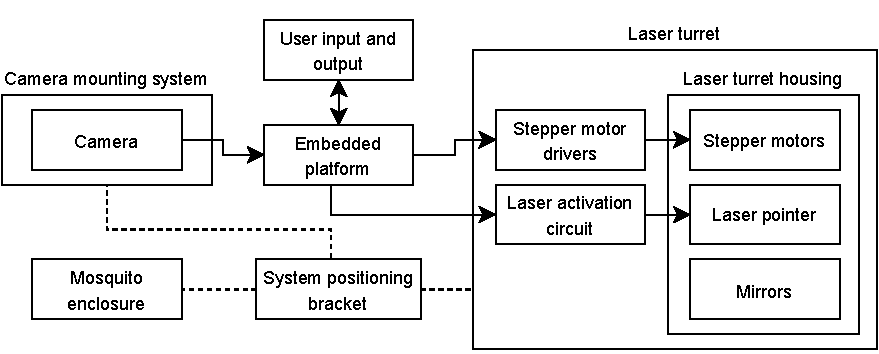
\includegraphics[width=\textwidth]{figures/hardware_block_diagram.pdf}
  \caption{System block diagram.}
\end{figure}


\subsection{Record 2.  Systems level description of the design}


\subsection{Record 3. Complete circuit diagrams and description}


\subsection{Record 4. Hardware acceptance test procedure}


\subsection{Record 5. User guide}


%% --------------------------------------------------------------------

\section{SOFTWARE part of the project}

\subsection{Record 6. Software process flow diagrams}
\begin{figure}[h]
  \centering
  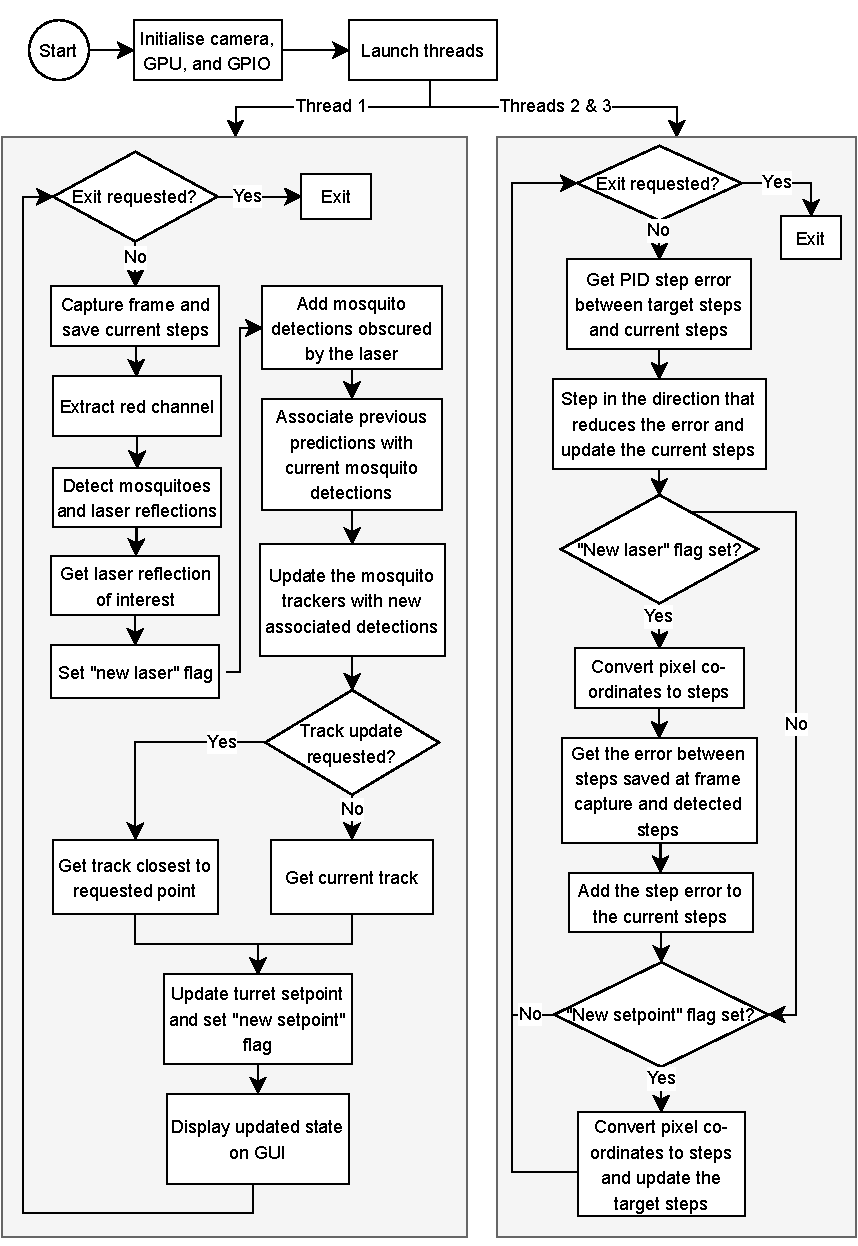
\includegraphics[width=0.95\textwidth]{figures/software_flow_diagram.pdf}
  \caption{Software flow diagram.}
\end{figure}


\subsection{Record 7. Explanation of software modules}


\subsection{Record 8. Complete source code}
Complete code has been submitted separately on the AMS.


\subsection{Record 9. Software acceptance test procedure}


\subsection{Record 10. Software user guide}


%% --------------------------------------------------------------------

\section{EXPERIMENTAL DATA}

\subsection{Record 11. Experimental data}


%% End of File.




\end{document}

%% End of File.
